\PassOptionsToPackage{unicode=true}{hyperref} % options for packages loaded elsewhere
\PassOptionsToPackage{hyphens}{url}
%


\documentclass[]{article}

\usepackage{ctex}
\setCJKmainfont{SimSun}
\usepackage{xeCJK} % 中文支持
\setCJKmainfont{Noto Serif CJK SC} % 设置中文字体为宋体
\usepackage{lmodern}
\usepackage{amssymb,amsmath}
\usepackage{ifxetex,ifluatex}
\usepackage{fixltx2e} % provides \textsubscript
\ifnum 0\ifxetex 1\fi\ifluatex 1\fi=0 % if pdftex
  \usepackage[T1]{fontenc}
  \usepackage[utf8]{inputenc}
  \usepackage{textcomp} % provides euro and other symbols
\else % if luatex or xelatex
  \usepackage{unicode-math}
  \defaultfontfeatures{Ligatures=TeX,Scale=MatchLowercase}
\fi
% use upquote if available, for straight quotes in verbatim environments
\IfFileExists{upquote.sty}{\usepackage{upquote}}{}
% use microtype if available
\IfFileExists{microtype.sty}{%
\usepackage[]{microtype}
\UseMicrotypeSet[protrusion]{basicmath} % disable protrusion for tt fonts
}{}
\IfFileExists{parskip.sty}{%
\usepackage{parskip}
}{% else
\setlength{\parindent}{0pt}
\setlength{\parskip}{6pt plus 2pt minus 1pt}
}
\usepackage{hyperref}
\hypersetup{
            pdfborder={0 0 0},
            breaklinks=true}
\urlstyle{same}  % don't use monospace font for urls
\usepackage{longtable,booktabs}
% Fix footnotes in tables (requires footnote package)
\IfFileExists{footnote.sty}{\usepackage{footnote}\makesavenoteenv{longtable}}{}
\usepackage{graphicx,grffile}
% 控制局部行间距
\usepackage{setspace}
\makeatletter
\def\maxwidth{\ifdim\Gin@nat@width>\linewidth\linewidth\else\Gin@nat@width\fi}
\def\maxheight{\ifdim\Gin@nat@height>\textheight\textheight\else\Gin@nat@height\fi}
\makeatother
% Scale images if necessary, so that they will not overflow the page
% margins by default, and it is still possible to overwrite the defaults
% using explicit options in \includegraphics[width, height, ...]{}
\setkeys{Gin}{width=\maxwidth,height=\maxheight,keepaspectratio}
\setlength{\emergencystretch}{3em}  % prevent overfull lines
\providecommand{\tightlist}{%
  \setlength{\itemsep}{0pt}\setlength{\parskip}{0pt}}
\setcounter{secnumdepth}{3}
% Redefines (sub)paragraphs to behave more like sections
\ifx\paragraph\undefined\else
\let\oldparagraph\paragraph
\renewcommand{\paragraph}[1]{\oldparagraph{#1}\mbox{}}
\fi
\ifx\subparagraph\undefined\else
\let\oldsubparagraph\subparagraph
\renewcommand{\subparagraph}[1]{\oldsubparagraph{#1}\mbox{}}
\fi

% set default figure placement to htbp
\makeatletter
\def\fps@figure{htbp}
\makeatother


\date{}

\begin{document}

\begin{center}
\protect\hypertarget{_Hlk208135206}{}{}
% 小一 ≈ 24pt
{\fontsize{24}{30}\selectfont 商业综合体信息管理系统}\\[8pt]
% 小二 ≈ 18pt
{\fontsize{18}{28}\selectfont\textbf{系统设计与实现文档}}\\[12pt]
% 名单使用小二,并通过 setspace 增加行间距
{\begin{spacing}{1.6}\fontsize{18}{28}\selectfont
2351454\quad 黄文\\
2353935\quad 刘逸飞\\
2251597\quad 韦瑾钰\\
2353926\quad 赵泽远\\
2351041\quad 刘浩田\\
2351880\quad 郑淑涵\\
2350284\quad 张俊峰\\
2352736\quad 孙一宁\\
2250832\quad 李杜若
\end{spacing}}
\end{center}

\newpage



\bigskip
目 录

\protect\hyperlink{_Toc77076512}{{1.} 商业综合体信息管理{系统需求} 1}

\protect\hyperlink{ux7cfbux7edfux529fux80fdux6027ux9700ux6c42}{1.1
  系统功能性需求 1}

\protect\hyperlink{ux7528ux6237ux767bux5f55ux529fux80fdux6570ux636eux9700ux6c42}{1.1.1
  用户登录功能数据需求 1}

\protect\hyperlink{ux7528ux6237ux6ce8ux518cux529fux80fdux6570ux636eux9700ux6c42}{1.1.2
  用户注册功能数据需求 1}

\protect\hyperlink{ux7528ux6237ux4fe1ux606fux7ba1ux7406ux529fux80fdux6570ux636eux9700ux6c42}{1.1.3
  用户信息管理功能数据需求 1}

\protect\hyperlink{ux533aux57dfux4fe1ux606fux7ba1ux7406ux529fux80fdux6570ux636eux9700ux6c42}{1.1.4
  区域信息管理功能数据需求 1}

\protect\hyperlink{ux5408ux4f5cux65b9ux4fe1ux606fux67e5ux8be2ux529fux80fdux6570ux636eux9700ux6c42}{1.1.5
  合作方信息查询功能数据需求 2}

\protect\hyperlink{ux5408ux4f5cux65b9ux4fe1ux606fux4feeux6539ux529fux80fdux6570ux636eux9700ux6c42}{1.1.6
  合作方信息修改功能数据需求 2}

\protect\hyperlink{ux5408ux4f5cux65b9ux7edfux8ba1ux4fe1ux606fux62a5ux8868ux6570ux636eux9700ux6c42}{1.1.7
  合作方统计信息报表数据需求 2}

\protect\hyperlink{ux573aux5730ux9884ux7ea6ux529fux80fdux6570ux636eux9700ux6c42}{1.1.8
  场地预约功能数据需求 2}

\protect\hyperlink{ux573aux5730ux6d3bux52a8ux7ba1ux7406ux529fux80fdux6570ux636eux9700ux6c42}{1.1.9
  场地活动管理功能数据需求 2}

\protect\hyperlink{ux573aux5730ux6d3bux52a8ux7ed3ux7b97ux6536ux8d39ux529fux80fdux6570ux636eux9700ux6c42}{1.1.10
  场地活动结算收费功能数据需求 2}

\protect\hyperlink{ux573aux5730ux6d3bux52a8ux7edfux8ba1ux6570ux636eux62a5ux8868ux751fux6210ux529fux80fd}{1.1.11
  场地活动统计数据报表生成功能 3}

\protect\hyperlink{ux4fc3ux9500ux6d3bux52a8ux7ba1ux7406ux529fux80fdux6570ux636eux9700ux6c42}{1.1.12
  促销活动管理功能数据需求 3}

\protect\hyperlink{ux4fc3ux9500ux6d3bux52a8ux7edfux8ba1ux6570ux636eux62a5ux8868ux751fux6210ux529fux80fd}{1.1.13
  促销活动统计数据报表生成功能 3}

\protect\hyperlink{ux5458ux5de5ux6743ux9650ux7ba1ux7406ux529fux80fdux6570ux636eux9700ux6c42}{1.1.14
  员工权限管理功能数据需求 3}

\protect\hyperlink{ux5458ux5de5ux4e2aux4ebaux4fe1ux606fux4feeux6539ux529fux80fdux6570ux636eux9700ux6c42}{1.1.15
  员工个人信息修改功能数据需求 3}

\protect\hyperlink{ux5458ux5de5ux8003ux52e4ux529fux80fdux6570ux636eux9700ux6c42}{1.1.16
  员工考勤功能数据需求 3}

\protect\hyperlink{ux5458ux5de5ux5de5ux8d44ux7ba1ux7406ux529fux80fdux6570ux636eux9700ux6c42}{1.1.17
  员工工资管理功能数据需求 4}

\protect\hyperlink{ux5458ux5de5ux5de5ux8d44ux7edfux8ba1ux62a5ux8868ux751fux6210ux529fux80fdux6570ux636eux9700ux6c42}{1.1.18
  员工工资统计报表生成功能数据需求 4}

\protect\hyperlink{ux5458ux5de5ux4e34ux65f6ux6743ux9650ux7ba1ux7406ux529fux80fdux6570ux636eux9700ux6c42}{1.1.19
  员工临时权限管理功能数据需求 4}

\protect\hyperlink{ux5546ux6237ux4fe1ux606fux7ba1ux7406ux529fux80fdux6570ux636eux9700ux6c42}{1.1.20
  商户信息管理功能数据需求 4}

\protect\hyperlink{ux5e97ux9762ux72b6ux6001ux7ba1ux7406ux529fux80fdux6570ux636eux9700ux6c42}{1.1.21
  店面状态管理功能数据需求 4}

\protect\hyperlink{ux5546ux6237ux4fe1ux606fux7edfux8ba1ux62a5ux8868ux529fux80fdux6570ux636eux9700ux6c42}{1.1.22
  商户信息统计报表功能数据需求 4}

\protect\hyperlink{ux5546ux6237ux79dfux91d1ux6536ux53d6ux529fux80fdux6570ux636eux9700ux6c42}{1.1.23
  商户租金收取功能数据需求 4}

\protect\hyperlink{ux5546ux6237ux79dfux91d1ux7edfux8ba1ux62a5ux8868ux529fux80fdux6570ux636eux9700ux6c42}{1.1.24
  商户租金统计报表功能数据需求 5}

\protect\hyperlink{ux505cux8f66ux573aux8f66ux4f4dux72b6ux6001ux67e5ux8be2ux529fux80fdux6570ux636eux9700ux6c42}{1.1.25
  停车场车位状态查询功能数据需求 5}

\protect\hyperlink{ux505cux8f66ux573aux51faux5165ux8f66ux8ba1ux8d39ux529fux80fdux6570ux636eux9700ux6c42}{1.1.26
  停车场出入车计费功能数据需求 5}

\protect\hyperlink{ux505cux8f66ux573aux7edfux8ba1ux4fe1ux606fux62a5ux8868ux529fux80fdux6570ux636eux9700ux6c42}{1.1.27
  停车场统计信息报表功能数据需求 5}

\protect\hyperlink{ux8bbeux5907ux76d1ux63a7ux548cux64cdux4f5cux529fux80fdux6570ux636eux9700ux6c42}{1.1.28
  设备监控和操作功能数据需求 5}

\protect\hyperlink{ux8bbeux5907ux7ef4ux62a4ux5de5ux5355ux529fux80fdux6570ux636eux9700ux6c42}{1.1.29
  设备维护工单功能数据需求 5}

\protect\hyperlink{ux7efcux5408ux73b0ux91d1ux6d41ux62a5ux8868ux529fux80fdux6570ux636eux9700ux6c42}{1.1.30
  综合现金流报表功能数据需求 5}

\protect\hyperlink{ux7cfbux7edfux975eux529fux80fdux6027ux9700ux6c42}{1.2
  系统非功能性需求 6}

\protect\hyperlink{ux6027ux80fdux9700ux6c42}{1.2.1 性能需求 6}

\protect\hyperlink{ux53efux9760ux6027ux9700ux6c42}{1.2.2 可靠性需求 6}

\protect\hyperlink{ux517cux5bb9ux6027ux9700ux6c42}{1.2.3 兼容性需求 6}

\protect\hyperlink{ux73afux5883ux9700ux6c42}{1.2.4 环境需求 6}

\protect\hyperlink{ux53efux9760ux6027ux9700ux6c42-1}{1.2.5 可靠性需求 6}

\protect\hyperlink{ux53efux6d4bux8bd5ux6027ux9700ux6c42}{1.2.6
  可测试性需求 6}

\protect\hyperlink{_Toc77076515}{{1.3} {组织结构} 1}

\protect\hyperlink{ux5546ux4e1aux7efcux5408ux4f53ux4fe1ux606fux7ba1ux7406ux7cfbux7edfux8bbeux8ba1ux4e0eux5b9eux73b0}{{2.}
商业综合体信息管理{系统设计与实现} 2}

\protect\hyperlink{ux7528ux6237ux7528ux4f8b}{{2.1} {**用例} 2}

\protect\hyperlink{ux7528ux6237ux7528ux4f8bux8bbeux8ba1}{{2.1.1}
    {**用例设计} 2}

\protect\hyperlink{ux7528ux6237ux7528ux4f8bux5b9eux73b0}{{2.1.2}
    {**用例实现} 2}

\protect\hyperlink{ux7528ux4f8b}{{2.2} {**用例} 3}

\protect\hyperlink{ux6570ux636eux5e93ux8bbeux8ba1}{{3.} {数据库设计} 4}

\protect\hyperlink{_Toc77076522}{{附录A.} {图表索引} 5}

\hypertarget{ux7cfbux7edfux9700ux6c42ux6982ux8ff0}{%
  \section{系统需求概述}\label{ux7cfbux7edfux9700ux6c42ux6982ux8ff0}}

本系统是为商业综合体管理人员设计的综合性信息管理平台,通过权限控制实现差异化数据访问和操作。系统涵盖区域管理、店铺管理、停车场管理、场地活动管理、设备管理、合作管理、员工权限管理、日志管理八大核心板块,支持业务流程闭环管理和数据分析功能。

\hypertarget{ux7cfbux7edfux529fux80fdux6027ux9700ux6c42}{%
  \subsection{系统功能性需求}\label{ux7cfbux7edfux529fux80fdux6027ux9700ux6c42}}

\hypertarget{ux7528ux6237ux767bux5f55ux529fux80fdux6570ux636eux9700ux6c42}{%
  \subsubsection{用户登录功能数据需求}\label{ux7528ux6237ux767bux5f55ux529fux80fdux6570ux636eux9700ux6c42}}

用户可以在首页进行登录。登录后则根据用户所属的权限分别跳转到员工界面/合作方界面/商户界面/管理员界面。在跳转后的页面可进行退出登录操作。

登录所需数据中用户名必须在3-10个字符之间,密码必须在6-15个字符之间,只能由ASCLL码表中可见字符组成,并且在数据库中加密存储。

\textbf{所需数据}:用户名、密码

\hypertarget{ux7528ux6237ux6ce8ux518cux529fux80fdux6570ux636eux9700ux6c42}{%
  \subsubsection{用户注册功能数据需求}\label{ux7528ux6237ux6ce8ux518cux529fux80fdux6570ux636eux9700ux6c42}}

用户可以在首页进行注册,注册可选员工/合作方/商户。注册后将到登录页面。

注册所需数据中用户名必须在3-10个字符之间且在数据库中没有重复,密码必须在6-15个字符之间,只能由ASCLL码表中可见字符组成,并且在数据库中加密存储。联系方式需要验证码验证。

第一个注册的用户会成为最高权限的管理员,并且可以指定其他新管理员,任何管理员可以修改其他非管理员用户的身份。

\textbf{所需数据}:用户名、密码、联系方式

\hypertarget{ux7528ux6237ux4fe1ux606fux7ba1ux7406ux529fux80fdux6570ux636eux9700ux6c42}{%
  \subsubsection{用户信息管理功能数据需求}\label{ux7528ux6237ux4fe1ux606fux7ba1ux7406ux529fux80fdux6570ux636eux9700ux6c42}}

用户可在登录后进入个人信息页面查看和修改个人信息,系统将根据用户身份限制可修改字段范围,修改后数据实时更新至数据库,用户可主动退出或保存后返回主界面。

\textbf{所需数据:}用户名、密码、联系方式、身份类型、所属部门、长期职位、可修改字段列表(如邮箱、电话、头像、紧急联系人)区域信息查询功能数据需求

\hypertarget{ux533aux57dfux4fe1ux606fux7ba1ux7406ux529fux80fdux6570ux636eux9700ux6c42}{%
  \subsubsection{区域信息管理功能数据需求}\label{ux533aux57dfux4fe1ux606fux7ba1ux7406ux529fux80fdux6570ux636eux9700ux6c42}}

拥有查询权限的管理人员可按区域ID、楼层、类型或空置状态检索区域信息,系统返回区域ID、是否空置、面积、类别、店面租金、场地费及当前租户或用途信息,查询结果支持列表与地图视图.

\textbf{所需数据}:账号权限、区域ID、楼层类型、空置状态

\hypertarget{ux5408ux4f5cux65b9ux4fe1ux606fux67e5ux8be2ux529fux80fdux6570ux636eux9700ux6c42}{%
  \subsubsection{合作方信息查询功能数据需求}\label{ux5408ux4f5cux65b9ux4fe1ux606fux67e5ux8be2ux529fux80fdux6570ux636eux9700ux6c42}}

权限达标的管理人员可查询合作方详细信息,包括联系方式和负责人信息。

合作对象ID为唯一标识符,联系方式需包含电话和邮箱。

\textbf{所需数据}:账号权限、合作对象ID、合作方名称、负责人姓名、联系方式

\hypertarget{ux5408ux4f5cux65b9ux4fe1ux606fux4feeux6539ux529fux80fdux6570ux636eux9700ux6c42}{%
  \subsubsection{合作方信息修改功能数据需求}\label{ux5408ux4f5cux65b9ux4fe1ux606fux4feeux6539ux529fux80fdux6570ux636eux9700ux6c42}}

项目经理可修改合作方信息及关联活动状态,需权限校验。

合作活动申请状态包括"审批中/进行中/已完成"三种状态。

\textbf{所需数据}:账号权限、合作对象ID、合作方名称、负责人姓名、联系方式、合作活动申请状态

\hypertarget{ux5408ux4f5cux65b9ux7edfux8ba1ux4fe1ux606fux62a5ux8868ux6570ux636eux9700ux6c42}{%
  \subsubsection{合作方统计信息报表数据需求}\label{ux5408ux4f5cux65b9ux7edfux8ba1ux4fe1ux606fux62a5ux8868ux6570ux636eux9700ux6c42}}

系统按月/季度/年生成合作方统计报表,包含合作方总数、活动次数、总投资金额、平均活动收益、活跃合作方排名,支持按时间段、行业类型筛选并以图表和表格形式导出.

\textbf{所需数据}:时间范围、合作方ID、活动ID、投资金额、活动收入、行业分类

\hypertarget{ux573aux5730ux9884ux7ea6ux529fux80fdux6570ux636eux9700ux6c42}{%
  \subsubsection{场地预约功能数据需求}\label{ux573aux5730ux9884ux7ea6ux529fux80fdux6570ux636eux9700ux6c42}}

项目经理填写活动场地预约申请,由权限达标的管理人员审批。

租用时间需满足"结束时间\textgreater{}起始时间"规则,活动区域ID需为有效编码。

\textbf{所需数据}:合作对象ID、活动区域ID、租用起始时间、租用结束时间、租用用途、合作方名称、员工职位

\hypertarget{ux573aux5730ux6d3bux52a8ux7ba1ux7406ux529fux80fdux6570ux636eux9700ux6c42}{%
  \subsubsection{场地活动管理功能数据需求}\label{ux573aux5730ux6d3bux52a8ux7ba1ux7406ux529fux80fdux6570ux636eux9700ux6c42}}

活动获批后生成活动记录,项目经理可更新活动名称、参与人数、内容描述、状态(筹备中/进行中/已结束),系统记录修改日志,支持批量导入参与人员。

\textbf{所需数据}:活动ID、活动名、活动人数、内容描述、活动状态、账号权限、临时权限ID

\hypertarget{ux573aux5730ux6d3bux52a8ux7ed3ux7b97ux6536ux8d39ux529fux80fdux6570ux636eux9700ux6c42}{%
  \subsubsection{场地活动结算收费功能数据需求}\label{ux573aux5730ux6d3bux52a8ux7ed3ux7b97ux6536ux8d39ux529fux80fdux6570ux636eux9700ux6c42}}

活动结束后系统根据实际使用时长、场地费标准及附加服务自动生成结算单,项目经理确认后生成应收款,支持在线支付与发票申请。

\textbf{所需数据}:活动ID、活动区域ID、租用起始时间、租用结束时间、场地费、附加服务费、支付方式、开票信息

\hypertarget{ux573aux5730ux6d3bux52a8ux7edfux8ba1ux6570ux636eux62a5ux8868ux751fux6210ux529fux80fd}{%
  \subsubsection{场地活动统计数据报表生成功能}\label{ux573aux5730ux6d3bux52a8ux7edfux8ba1ux6570ux636eux62a5ux8868ux751fux6210ux529fux80fdux6570ux636eux9700ux6c42}}

系统按日/周/月生成场地活动统计报表,包含活动场次、总租用时长、总收费、平均上座率、热门场地排行,可导出PDF/Excel。

\textbf{所需数据}:活动ID、活动区域ID、租用起始时间、租用结束时间、场地费、实际参与人数

\hypertarget{ux4fc3ux9500ux6d3bux52a8ux7ba1ux7406ux529fux80fdux6570ux636eux9700ux6c42}{%
  \subsubsection{促销活动管理功能数据需求}\label{ux4fc3ux9500ux6d3bux52a8ux7ba1ux7406ux529fux80fdux6570ux636eux9700ux6c42}}

管理员或商户可创建促销活动,填写活动名称、促销花费、目标店铺、开始结束时间、折扣或满减规则,系统自动推送至关联店铺。

\textbf{所需数据}:活动ID、活动名称、促销花费、店铺ID列表、活动开始时间、活动结束时间、促销规则描述

\hypertarget{ux4fc3ux9500ux6d3bux52a8ux7edfux8ba1ux6570ux636eux62a5ux8868ux751fux6210ux529fux80fd}{%
  \subsubsection{促销活动统计数据报表生成功能}\label{ux4fc3ux9500ux6d3bux52a8ux7edfux8ba1ux6570ux636eux62a5ux8868ux751fux6210ux529fux80fdux6570ux636eux9700ux6c42}}

系统在促销活动结束后生成效果报表,包括参与店铺数、总销售额增量、促销成本、ROI、优惠券核销率,支持按店铺或活动维度对比。

\textbf{所需数据}:活动ID、店铺ID、促销花费、销售额增量、优惠券使用量、时间范围

\hypertarget{ux5458ux5de5ux6743ux9650ux7ba1ux7406ux529fux80fdux6570ux636eux9700ux6c42}{%
  \subsubsection{员工权限管理功能数据需求}\label{ux5458ux5de5ux6743ux9650ux7ba1ux7406ux529fux80fdux6570ux636eux9700ux6c42}}

人事管理员可新增、修改或撤销员工权限,权限按角色模板分配,变更即时生效并记录审计日志,支持批量导入与权限有效期设置。

\textbf{所需数据}:员工ID、账号权限、角色模板、授权管理员账号、生效时间、失效时间、变更原因

\hypertarget{ux5458ux5de5ux4e2aux4ebaux4fe1ux606fux4feeux6539ux529fux80fdux6570ux636eux9700ux6c42}{%
  \subsubsection{员工个人信息修改功能数据需求}\label{ux5458ux5de5ux4e2aux4ebaux4fe1ux606fux4feeux6539ux529fux80fdux6570ux636eux9700ux6c42}}

员工可在权限允许范围内修改个人非敏感信息,系统根据身份类型开放不同字段,修改后同步更新员工表与账号表,并记录修改日志。

\textbf{所需数据}:员工ID、可修改字段列表(如联系方式、紧急联系人、头像链接)、变更内容、修改时间、操作账号

\hypertarget{ux5458ux5de5ux8003ux52e4ux529fux80fdux6570ux636eux9700ux6c42}{%
  \subsubsection{员工考勤功能数据需求}\label{ux5458ux5de5ux8003ux52e4ux529fux80fdux6570ux636eux9700ux6c42}}

系统每日自动记录员工签到签退时间,允许补录与异常申诉,月末生成考勤汇总。

\textbf{所需数据}:员工ID、签到时间、签退时间、考勤状态(正常/迟到/早退/缺勤)、补录原因、申诉说明

\hypertarget{ux5458ux5de5ux5de5ux8d44ux7ba1ux7406ux529fux80fdux6570ux636eux9700ux6c42}{%
  \subsubsection{员工工资管理功能数据需求}\label{ux5458ux5de5ux5de5ux8d44ux7ba1ux7406ux529fux80fdux6570ux636eux9700ux6c42}}

人事部门每月根据考勤、奖金、罚金计算工资,支持批量导入与个别调整,工资单生成后员工可在线查看与确认。

\textbf{所需数据}:员工ID、底薪、奖金、罚金、考勤次数、实际薪水、发放月份、确认状态

\hypertarget{ux5458ux5de5ux5de5ux8d44ux7edfux8ba1ux62a5ux8868ux751fux6210ux529fux80fdux6570ux636eux9700ux6c42}{%
  \subsubsection{员工工资统计报表生成功能数据需求}\label{ux5458ux5de5ux5de5ux8d44ux7edfux8ba1ux62a5ux8868ux751fux6210ux529fux80fdux6570ux636eux9700ux6c42}}

员工工资统计报表生成功能数据需求
系统按月生成工资总览报表,包含部门工资总额、人均工资、最高最低值、奖金罚金分布,支持导出与图表展示。

\textbf{所需数据}:时间(月份)、员工ID、部门、底薪、奖金、罚金、实际薪水

\hypertarget{ux5458ux5de5ux4e34ux65f6ux6743ux9650ux7ba1ux7406ux529fux80fdux6570ux636eux9700ux6c42}{%
  \subsubsection{员工临时权限管理功能数据需求}\label{ux5458ux5de5ux4e34ux65f6ux6743ux9650ux7ba1ux7406ux529fux80fdux6570ux636eux9700ux6c42}}

项目经理可为活动临时授权员工,权限在活动结束后自动回收,系统记录授权与回收日志。

\textbf{所需数据}:授权人账号、员工ID、活动ID、临时权限内容、授权时间、回收时间、活动结束标记

\hypertarget{ux5546ux6237ux4fe1ux606fux7ba1ux7406ux529fux80fdux6570ux636eux9700ux6c42}{%
  \subsubsection{商户信息管理功能数据需求}\label{ux5546ux6237ux4fe1ux606fux7ba1ux7406ux529fux80fdux6570ux636eux9700ux6c42}}

管理人员可查看与更新店铺及租户信息,支持按店铺ID、租户名称、状态检索,修改后同步更新店铺表。

\textbf{所需数据}:店铺ID、店铺名称、店铺状态、租户类型、租户名、租户联系方式、租用起始时间、租用结束时间、租金提交状态

\hypertarget{ux5e97ux9762ux72b6ux6001ux7ba1ux7406ux529fux80fdux6570ux636eux9700ux6c42}{%
  \subsubsection{店面状态管理功能数据需求}\label{ux5e97ux9762ux72b6ux6001ux7ba1ux7406ux529fux80fdux6570ux636eux9700ux6c42}}

区域管理员可变更店面空置状态,更新租金或面积,变更前校验是否存在有效租约,所有变更记录入日志。

\textbf{所需数据}:区域ID、空置标识、面积、店铺租金、变更原因、操作账号

\hypertarget{ux5546ux6237ux4fe1ux606fux7edfux8ba1ux62a5ux8868ux529fux80fdux6570ux636eux9700ux6c42}{%
  \subsubsection{商户信息统计报表功能数据需求}\label{ux5546ux6237ux4fe1ux606fux7edfux8ba1ux62a5ux8868ux529fux80fdux6570ux636eux9700ux6c42}}

商户信息统计报表功能数据需求
系统实时生成商户运营报表,包含总店铺数、正常营业/空置/停业比例、租户行业分布、租金收缴率,可导出为PDF。

\textbf{所需数据}:店铺ID、店铺状态、租户类型、租用起始时间、租用结束时间、租金提交状态

\hypertarget{ux5546ux6237ux79dfux91d1ux6536ux53d6ux529fux80fdux6570ux636eux9700ux6c42}{%
  \subsubsection{商户租金收取功能数据需求}\label{ux5546ux6237ux79dfux91d1ux6536ux53d6ux529fux80fdux6570ux636eux9700ux6c42}}

租户登录店铺账号后查看应付租金并在线支付,系统生成电子收据并更新租金提交状态,逾期自动提醒。

\textbf{所需数据}:店铺ID、租户账号、应付金额、支付时间、支付方式、支付状态、收据编号

\hypertarget{ux5546ux6237ux79dfux91d1ux7edfux8ba1ux62a5ux8868ux529fux80fdux6570ux636eux9700ux6c42}{%
  \subsubsection{商户租金统计报表功能数据需求}\label{ux5546ux6237ux79dfux91d1ux7edfux8ba1ux62a5ux8868ux529fux80fdux6570ux636eux9700ux6c42}}

商户租金统计报表功能数据需求
系统按周期生成租金收入报表,展示应收、实收、欠费、逾期天数、收缴率及趋势图。

\textbf{所需数据}:店铺ID、区域ID、店面租金、租用起始时间、租用结束时间、租金提交状态、支付时间

\hypertarget{ux505cux8f66ux573aux8f66ux4f4dux72b6ux6001ux67e5ux8be2ux529fux80fdux6570ux636eux9700ux6c42}{%
  \subsubsection{停车场车位状态查询功能数据需求}\label{ux505cux8f66ux573aux8f66ux4f4dux72b6ux6001ux67e5ux8be2ux529fux80fdux6570ux636eux9700ux6c42}}

系统实时展示各停车场区域的车位占用情况,支持按区域、楼层、车位ID筛选,并提供剩余车位数统计。

\textbf{所需数据}:区域ID、车位ID、是否有车、更新时间、查询账号权限

\hypertarget{ux505cux8f66ux573aux51faux5165ux8f66ux8ba1ux8d39ux529fux80fdux6570ux636eux9700ux6c42}{%
  \subsubsection{停车场出入车计费功能数据需求}\label{ux505cux8f66ux573aux51faux5165ux8f66ux8ba1ux8d39ux529fux80fdux6570ux636eux9700ux6c42}}

车辆入场时自动抓拍车牌并分配车位,出场时按停车时长计费,支持现金、扫码、无感支付,系统记录完整流水。

\textbf{所需数据}:车牌号、区域ID、车位ID、停车起始时间、停车结束时间、单位时间停车费、支付状态

\hypertarget{ux505cux8f66ux573aux7edfux8ba1ux4fe1ux606fux62a5ux8868ux529fux80fdux6570ux636eux9700ux6c42}{%
  \subsubsection{停车场统计信息报表功能数据需求}\label{ux505cux8f66ux573aux7edfux8ba1ux4fe1ux606fux62a5ux8868ux529fux80fdux6570ux636eux9700ux6c42}}

系统按日/周/月生成停车场运营报表,包含车流量、收入总额、平均停车时长、高峰时段车位利用率,支持图表与Excel导出。

\textbf{所需数据}:区域ID、车牌号、停车起始时间、停车结束时间、单位时间停车费

\hypertarget{ux8bbeux5907ux76d1ux63a7ux548cux64cdux4f5cux529fux80fdux6570ux636eux9700ux6c42}{%
  \subsubsection{设备监控和操作功能数据需求}\label{ux8bbeux5907ux76d1ux63a7ux548cux64cdux4f5cux529fux80fdux6570ux636eux9700ux6c42}}

管理员可实时查看设备运行状态并进行远程控制,系统记录操作日志与状态变更,异常自动报警。

\textbf{所需数据}:设备ID、类别、状态、接口、区域ID、操作指令、操作账号、操作时间

\hypertarget{ux8bbeux5907ux7ef4ux62a4ux5de5ux5355ux529fux80fdux6570ux636eux9700ux6c42}{%
  \subsubsection{设备维护工单功能数据需求}\label{ux8bbeux5907ux7ef4ux62a4ux5de5ux5355ux529fux80fdux6570ux636eux9700ux6c42}}

报修人提交工单后系统分配维修员工,维修完成后填写结果与花费,所有流程状态可追踪。

\textbf{所需数据}:设备ID、员工ID、维修开始时间、维修结束时间、维修花费、故障描述、处理结果、工单状态

\hypertarget{ux7efcux5408ux73b0ux91d1ux6d41ux62a5ux8868ux529fux80fdux6570ux636eux9700ux6c42}{%
  \subsubsection{综合现金流报表功能数据需求}\label{ux7efcux5408ux73b0ux91d1ux6d41ux62a5ux8868ux529fux80fdux6570ux636eux9700ux6c42}}

综合现金流报表功能数据需求
系统每日自动汇总租金、停车费、活动收入、工资、维修、设备采购等现金收支,生成日报、月报、年报,支持按类别与时间段筛选。

\textbf{所需数据}:收入类型、支出类型、金额、发生时间、关联单据编号、账户余额

\hypertarget{ux7cfbux7edfux975eux529fux80fdux6027ux9700ux6c42}{%
  \subsection{系统非功能性需求}\label{ux7cfbux7edfux975eux529fux80fdux6027ux9700ux6c42}}

\hypertarget{ux6027ux80fdux9700ux6c42}{%
  \subsubsection{性能需求}\label{ux6027ux80fdux9700ux6c42}}

系统支持高效的数据查询与事务处理,可以确保在并发场景下稳定运行;后端部署于Ubuntu
22.04服务器,采用ASP.NET Core框架,前端基于Vue框架开发。

\textbf{所需数据}:操作系统,后端日志、前端框架、数据库、API 协议。

\hypertarget{ux53efux9760ux6027ux9700ux6c42}{%
  \subsubsection{可靠性需求}\label{ux53efux9760ux6027ux9700ux6c42}}

系统需具备高可用性,确保在长时间运行过程中稳定可靠。系统支持持续运行,减少计划外停机时间。

\textbf{所需数据}:系统可用性百分比、计划内维护时间、故障恢复时间(RTO)、数据恢复点(RPO)

\hypertarget{ux517cux5bb9ux6027ux9700ux6c42}{%
  \subsubsection{兼容性需求}\label{ux517cux5bb9ux6027ux9700ux6c42}}

系统需具备良好的兼容性,确保在不同环境下稳定运行。系统支持主流的浏览器和操作系统版本,确保前后端框架的兼容性。

\textbf{所需数据}:操作系统版本(Ubuntu 22.04)、后端框架版本(ASP.NET
Core)、前端框架版本(Vue)

\hypertarget{ux73afux5883ux9700ux6c42}{%
  \subsubsection{环境需求}\label{ux73afux5883ux9700ux6c42}}

系统运行环境基于 Ubuntu 22.04 操作系统,后端采用 ASP.NET Core
框架,前端使用 Vue 框架进行开发

\textbf{所需数据}:操作系统版本(Ubuntu 22.04)、后端框架版本(ASP.NET
Core)、前端框架版本(Vue)

\hypertarget{ux53efux9760ux6027ux9700ux6c42-1}{%
  \subsubsection{可靠性需求}\label{ux53efux9760ux6027ux9700ux6c42-1}}

系统需具备良好的可维护性,确保代码清晰、易于管理和更新。后端采用 ASP.NET
Core 框架,前端使用 Vue 框架,便于后续开发和维护

\textbf{所需数据}:代码规范、注释覆盖率、配置中心接口

\hypertarget{ux53efux6d4bux8bd5ux6027ux9700ux6c42}{%
  \subsubsection{可测试性需求}\label{ux53efux6d4bux8bd5ux6027ux9700ux6c42}}

系统需具备良好的可测试性,确保各功能模块能够进行有效的单元测试和集成测试。数据库设计中涉及的各个表和关系模式应支持独立测试,确保数据交互的准确性和完整性。同时,系统应支持对数据库操作的自动化测试,以验证数据的正确性和一致性

\textbf{所需数据}:单元测试覆盖率、接口自动化测试用例数、数据库操作测试覆盖率

\hypertarget{ux53efux7ef4ux62a4ux6027ux9700ux6c42}{%
  \subsubsection{可维护性需求}\label{ux53efux7ef4ux62a4ux6027ux9700ux6c42}}

系统需具备良好的可维护性,确保代码清晰、易于管理和更新。数据库设计应遵循规范化原则,确保数据结构合理,便于后续的扩展和维护。同时,系统应支持在线热更新配置,减少维护时间对业务的影响。

\textbf{所需数据}:数据库表结构设计文档、代码注释覆盖率、配置中心接口

\hypertarget{ux7ec4ux7ec7ux7ed3ux6784}{%
  \subsection{组织结构}\label{ux7ec4ux7ec7ux7ed3ux6784}}

列出文档的组织结构。

第一章:系统需求概述。展示我们设计的商业综合体信息管理系统的各功能对应的数据需求。

第二章:系统设计与实现。分析各系统功能的详细设计与代码实现。

第三章:数据库实现。分析数据库的具体实现。

附录A:是本文档的图表索引

\hypertarget{ux5546ux4e1aux7efcux5408ux4f53ux4fe1ux606fux7ba1ux7406ux7cfbux7edfux8bbeux8ba1ux4e0eux5b9eux73b0}{%
  \section{商业综合体信息管理系统设计与实现}\label{ux5546ux4e1aux7efcux5408ux4f53ux4fe1ux606fux7ba1ux7406ux7cfbux7edfux8bbeux8ba1ux4e0eux5b9eux73b0}}

本系统的使用者分为三类角色:管理员作为最高权限管理者,可全面掌控用户注册、区域划分、合作方审批、员工权限分配及现金流报表等核心功能;员工依据部门和职位权限,管理个人信息、考勤工资、活动申请及设备运维;商户则专注于自身店铺的运营,包括信息维护、租金缴纳、店面状态更新及促销活动参与。所有权限通过账号身份严格隔离。

\hypertarget{ux7528ux6237ux7528ux4f8b}{%
  \subsection{ 用户用例}\label{ux7528ux6237ux7528ux4f8b}}

\hypertarget{ux7528ux6237ux7528ux4f8bux8bbeux8ba1}{%
  \subsubsection{用户用例设计}\label{ux7528ux6237ux7528ux4f8bux8bbeux8ba1}}

\protect\hypertarget{_Toc153186375}{}{\protect\hypertarget{_Toc394245026}{}{}}表格
2‑1 用户功能的动作序列

\begin{longtable}[]{@{}ll@{}}
  \toprule
  动作序列 & 描述\tabularnewline
  \midrule
  \endhead
  登录   & 不同用户登录进入到不同页面。\tabularnewline
  注册   &
  访客在系统首页选择注册,填写必要信息后提交,系统校验并创建账号\tabularnewline
  修改信息 &
  用户进入``个人信息''页面,对可编辑字段进行修改并提交,系统校验后更新数据库\tabularnewline
  \bottomrule
\end{longtable}

用户登录活动图:

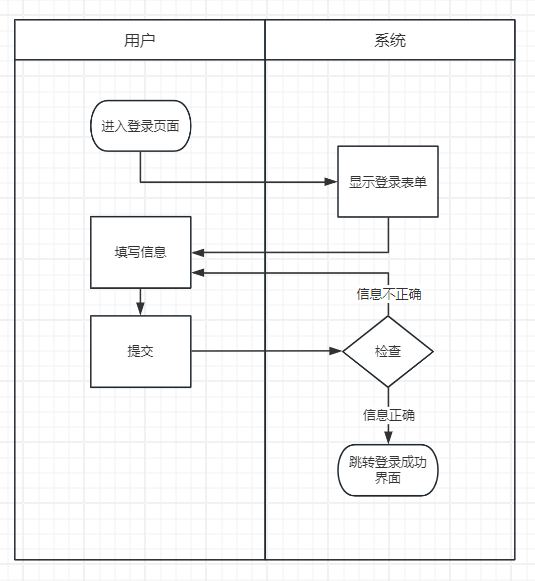
\includegraphics[width=4.45694in,height=4.83819in]{media/media/image1.png}

用户注册活动图:

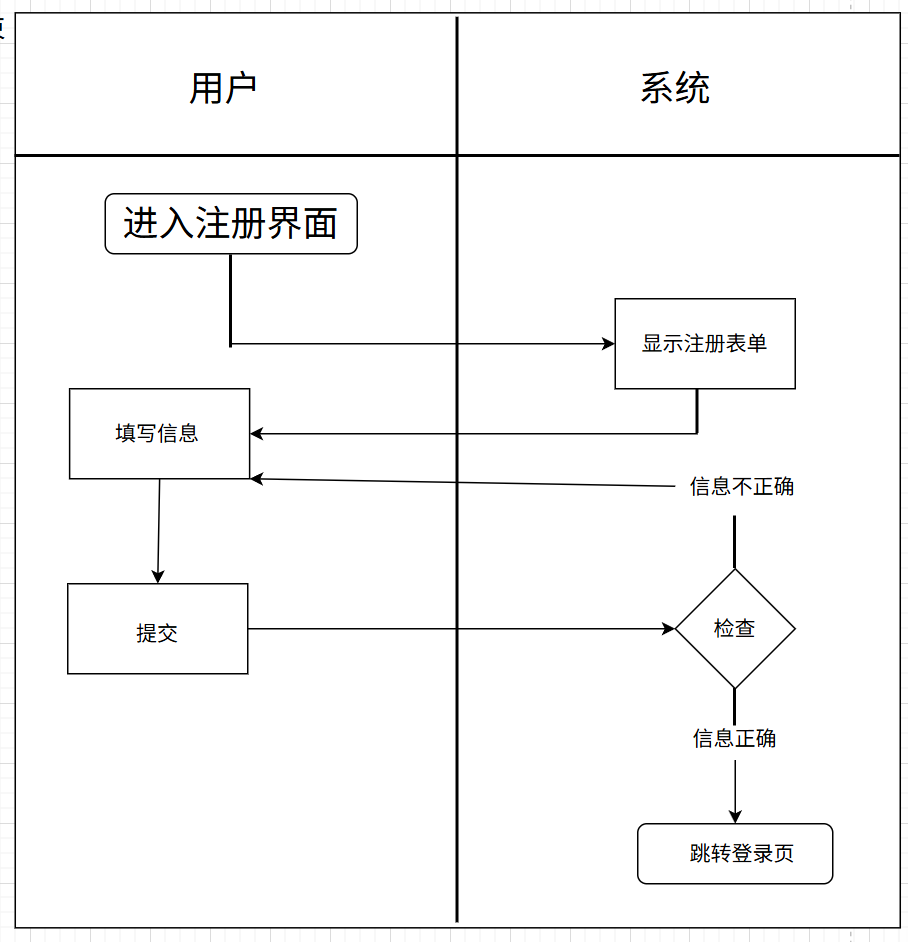
\includegraphics[width=4.35278in,height=4.51458in]{media/media/image2.png}

用户修改信息活动图:

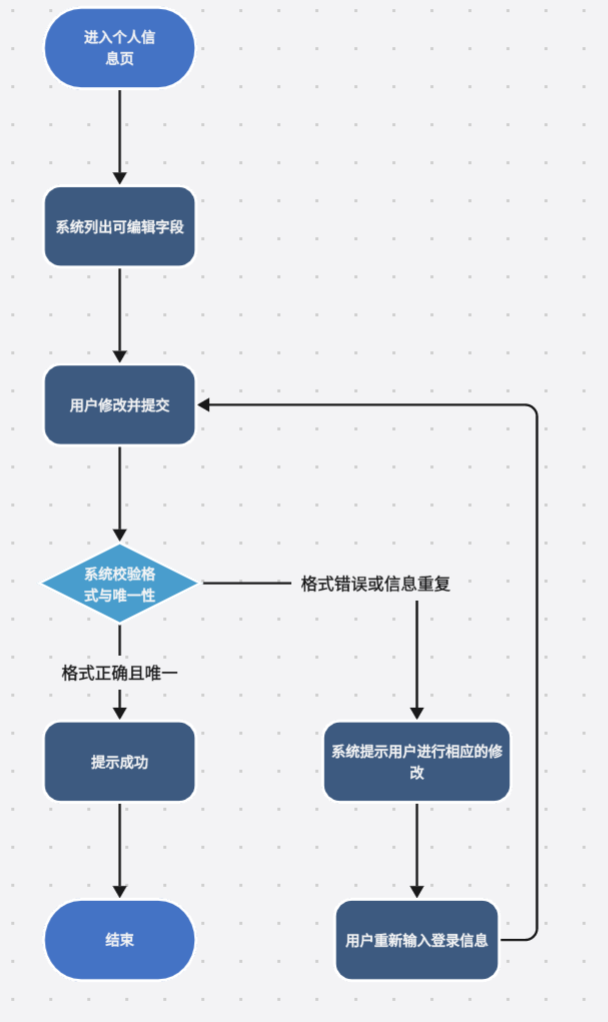
\includegraphics[width=2.82083in,height=4.73958in]{media/media/image3.png}

\hypertarget{ux7528ux6237ux7528ux4f8bux5b9eux73b0}{%
  \subsubsection{用户用例实现}\label{ux7528ux6237ux7528ux4f8bux5b9eux73b0}}

1. 主要类及其关系:

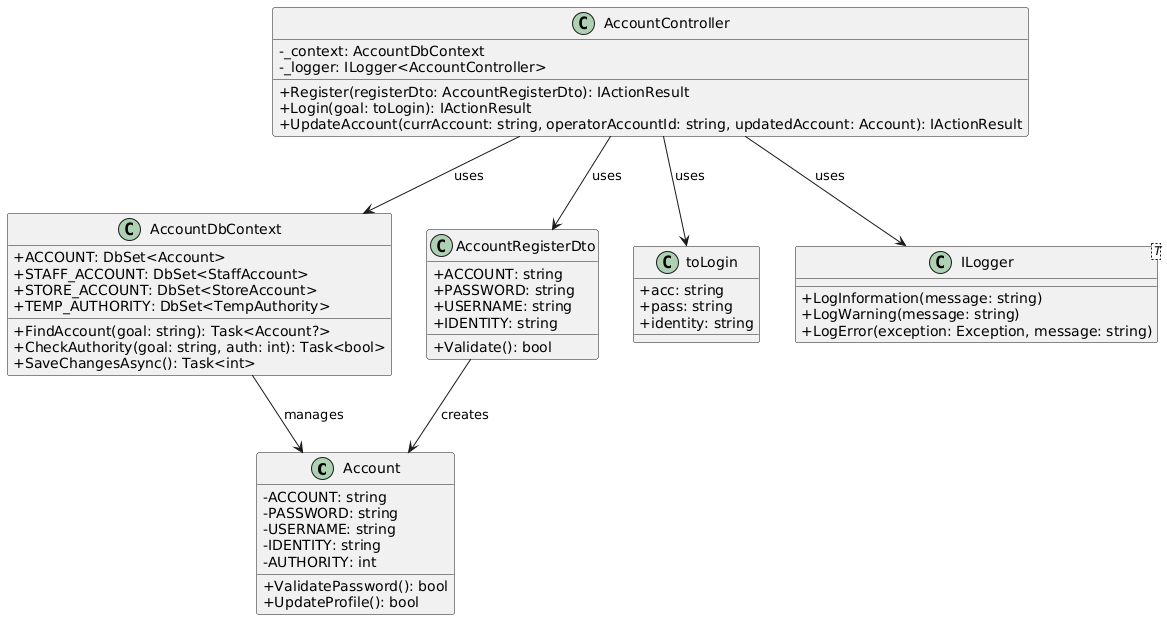
\includegraphics[width=6.06528in,height=3.22222in]{media/media/image4.png}

2. 方法设计与实现

用户登录:
\begin{verbatim}
public class toLogin
{
    public string acc { get; set; }
    public string pass { get; set; }
    public string identity { get; set; }
}

[HttpPost("login")]
public async Task<IActionResult> Login([FromBody] toLogin goal)
\end{verbatim}

验证用户身份并授权访问系统。该方法接收登录凭证后,首先查询数据库验证账号是否存在,随后校验密码是否匹配,最后核查账户状态是否可用(未被封禁)以及身份标识是否正确。全部验证通过后,返回该账户的完整信息以建立用户会话。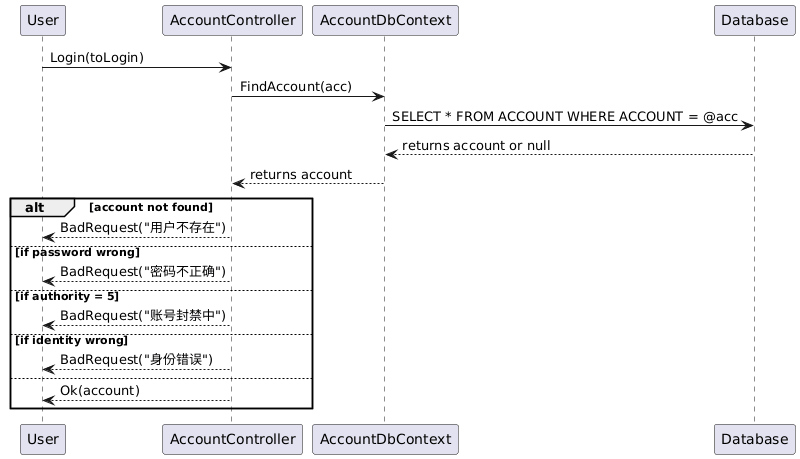
\includegraphics[width=5.88681in,height=3.37778in]{media/media/image5.png}

用户注册

在系统中创建新的用户账户。该方法会首先确保请求账号名的唯一性。对于系统首个注册的用户,将自动授予其最高管理员权限。后续注册则根据其选择的身份(``员工''或``商户'')分配相应的基础权限。最终,将新账户信息持久化至数据库,完成注册流程。
\begin{verbatim}
public class AccountRegisterDto{
    [Required(ErrorMessage = "账号为必填项")]
    [StringLength(50, MinimumLength = 3, ErrorMessage = "账号长度必须在3到50个字符之间")]
    public string ACCOUNT { get; set; }
    [Required(ErrorMessage = "密码为必填项")]
    [StringLength(100, MinimumLength = 6, ErrorMessage = "密码长度至少为6个字符")]
    public string PASSWORD { get; set; }
    [Required(ErrorMessage = "用户名为必填项")]
    [StringLength(50)]
    public string USERNAME { get; set; }
    [Required(ErrorMessage = "必须指定用户身份")]
    [StringLength(50)]
    public string IDENTITY { get; set; }
}

[HttpPost("register")]
public async Task<IActionResult> Register([FromBody] AccountRegisterDto registerDto)
\end{verbatim}

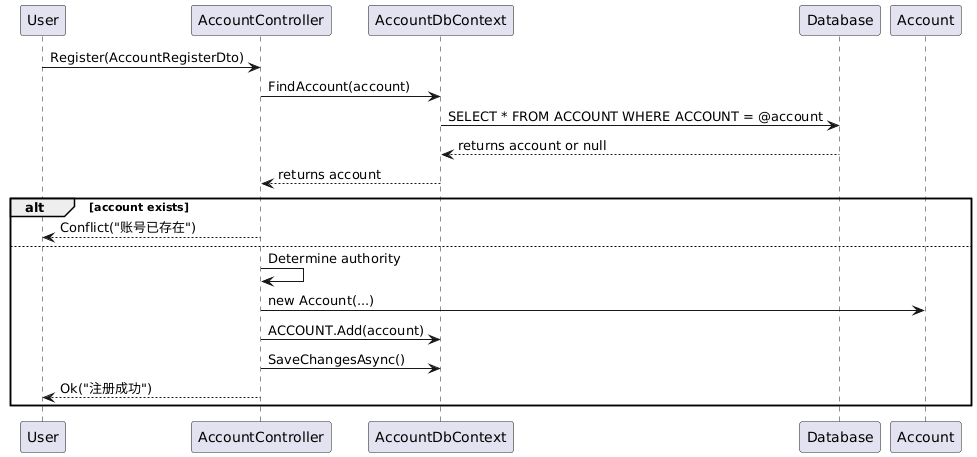
\includegraphics[width=5.75347in,height=2.69097in]{media/media/image6.png}

用户信息修改:

更新指定账户的详细信息。此操作需要由另一名已登录的操作员发起,并包含严格的权限校验逻辑以确保数据安全。仅允许系统管理员修改他人账户,且操作员的权限等级必须高于或等于其要修改的目标权限。该方法会防止关键字段(如账号名)被误修改,并确保身份等数据的有效性,最终将合规的变更安全地更新至数据库。
\begin{verbatim}
[HttpPatch("alter/{currAccount}")]
public async Task<IActionResult> UpdateAccount(
    string currAccount,
    [FromQuery] string operatorAccountId,
    [FromBody] Account updatedAccount)
\end{verbatim}

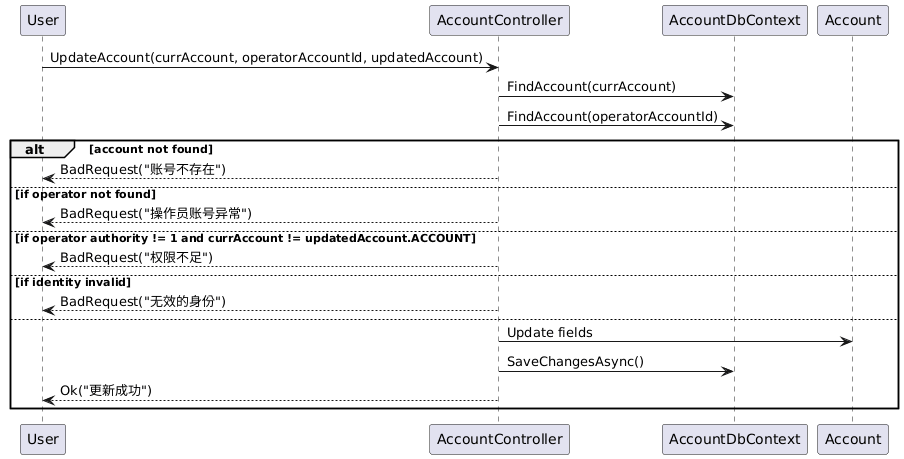
\includegraphics[width=5.64167in,height=2.86458in]{media/media/image7.png}

\hypertarget{ux7528ux4f8b}{%
  \subsection{**用例}\label{ux7528ux4f8b}}

依此类推。

\hypertarget{ux7528ux4f8b-1}{%
  \subsection{区域用例}\label{ux7528ux4f8b-1}}
\hypertarget{ux7528ux4f8b-1ux8bbeux8ba1}{%
  \subsubsection{区域用例设计}\label{ux7528ux4f8b-1ux8bbeux8ba1}}

% 区域用例设计表格

\begin{longtable}[]{@{}ll@{}}
  \toprule
  \textbf{动作序列} & \textbf{描述}                \\
  \midrule
  \endhead
  添加新区域         & 管理员在系统内新增一块可租用的区域,并设定其基础属性 \\
  区域信息查询        & 用户按条件检索区域列表并查看详情           \\
  区域信息管理        & 管理员对已有区域的基础属性进行修改或删除       \\
  \bottomrule
\end{longtable}

添加新区域活动图:

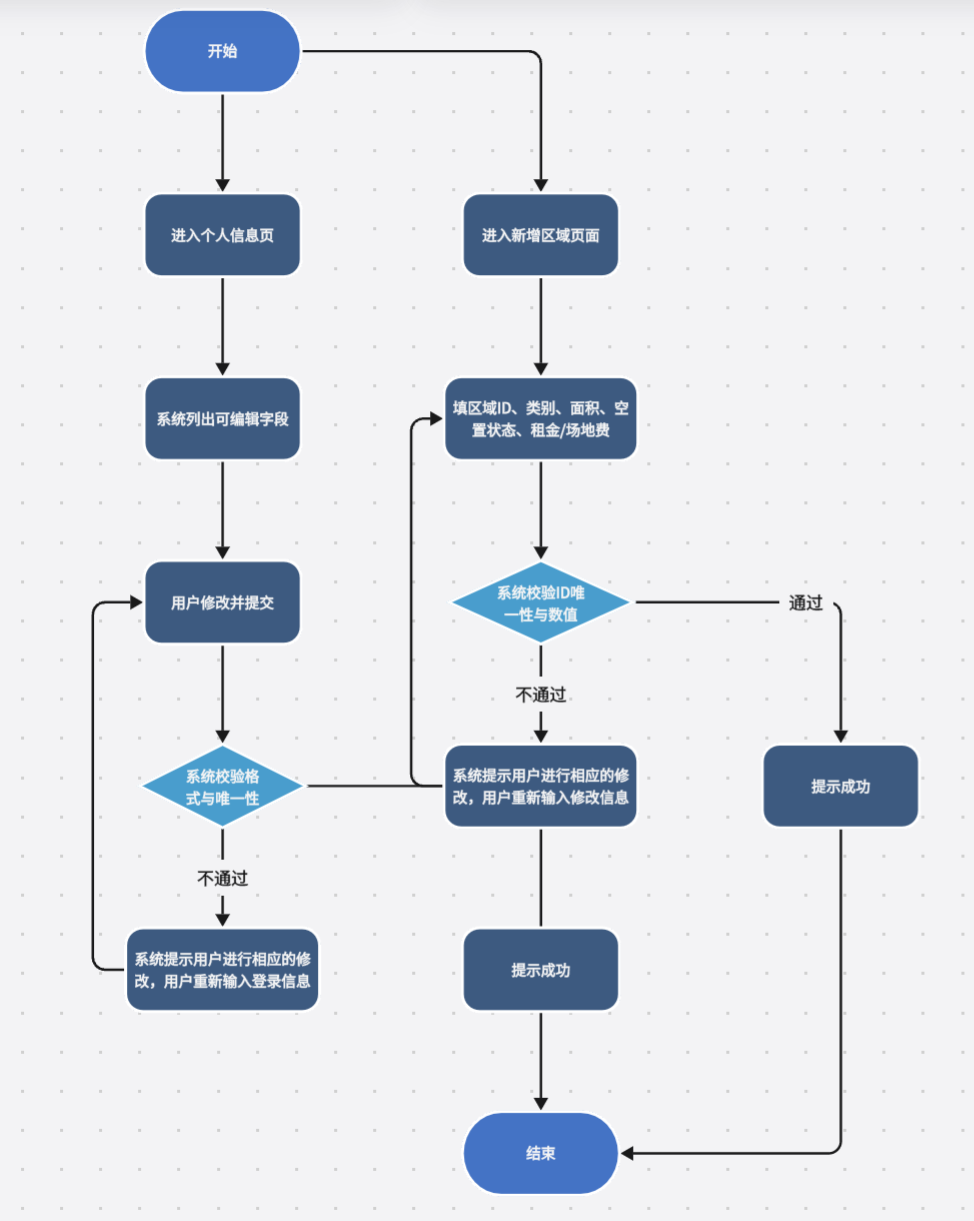
\includegraphics[width=4.45694in,height=4.83819in]{media/media/image_2-3-1.png}

区域信息查询活动图:

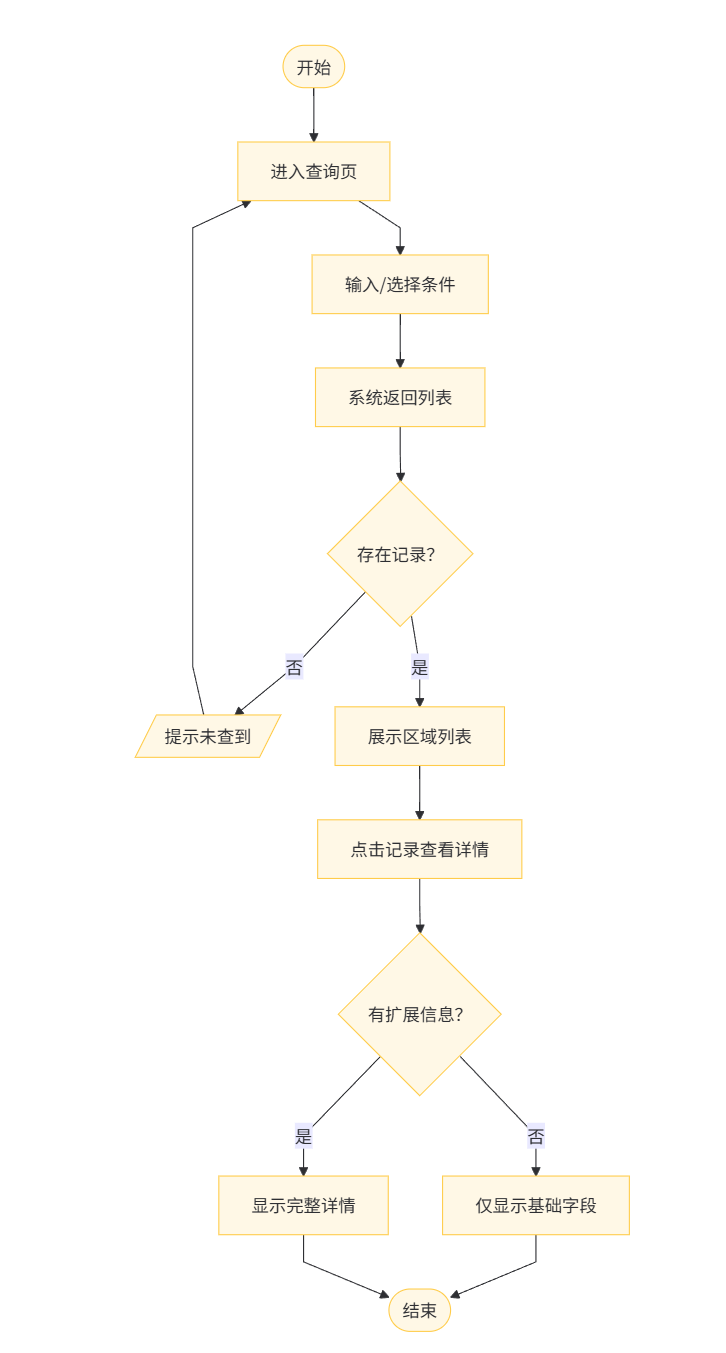
\includegraphics[width=4.45694in,height=4.83819in]{media/media/image_2-3-2.png}

区域信息管理活动图:

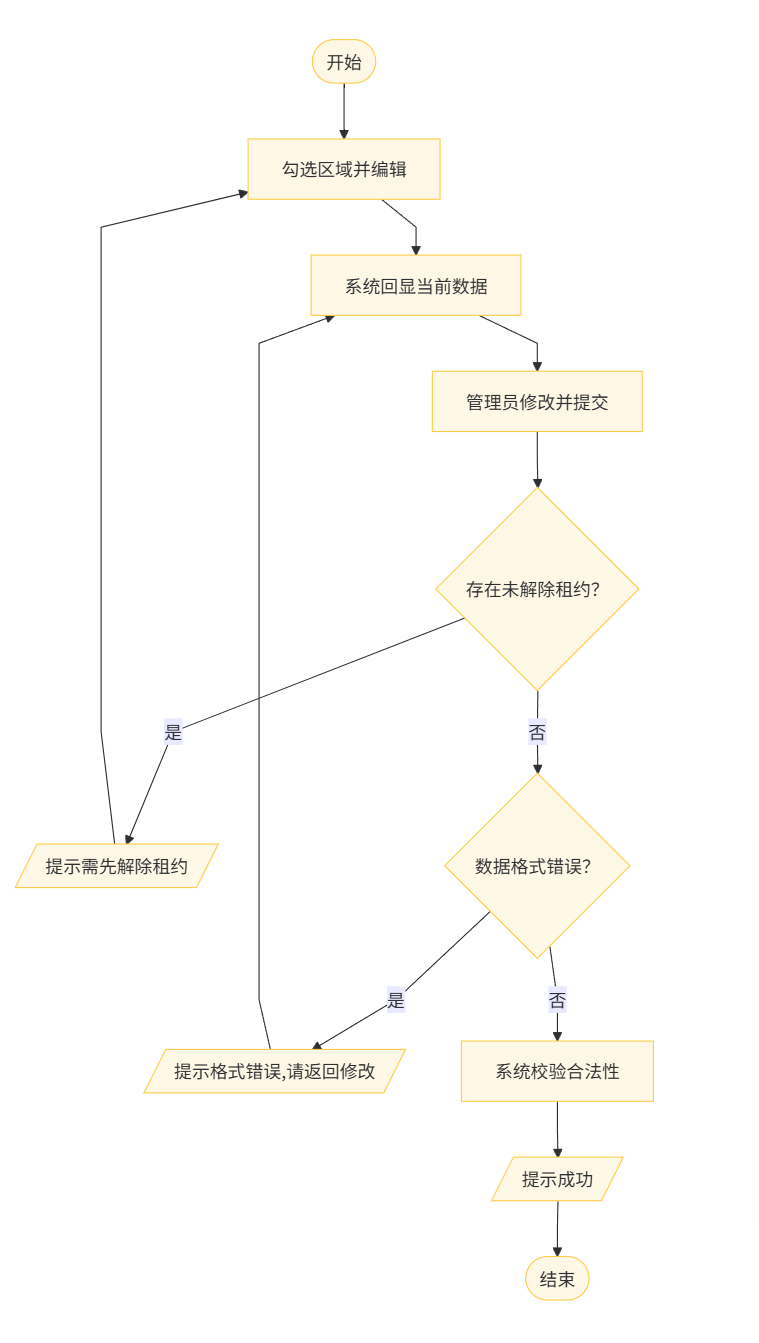
\includegraphics[width=4.45694in,height=4.83819in]{media/media/image_2-3-3.png}

\hypertarget{ux7528ux4f8b-1ux5b9eux73b0}{%
  \subsubsection{区域用例实现}\label{ux7528ux4f8b-1ux5b9eux73b0}}
1. 主要类及其关系:
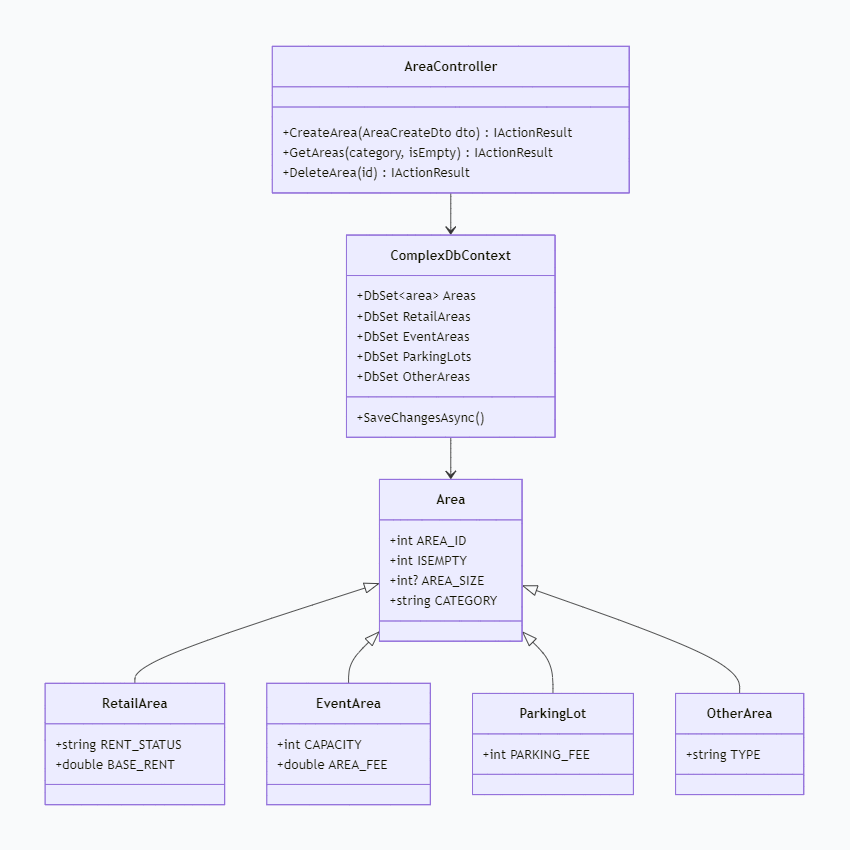
\includegraphics[width=6.06528in,height=3.22222in]{media/media/image_2-3-4.png}

2. 方法设计与实现

添加新区域

\begin{verbatim}
public class AreaCreateDto {
    public int AreaId { get; set; }
    public int IsEmpty { get; set; }
    public int? AreaSize { get; set; }
    [Required]
    public string Category { get; set; } // "RETAIL", "EVENT"
    // Retail-specific properties
    public string? RentStatus { get; set; }
    public double? BaseRent { get; set; }
    // Event-specific properties
    public int? Capacity { get; set; }
    public int? AreaFee { get; set; }
    // 其它类型
    public string? Type { get; set; }
    public int? ParkingFee { get; set; }
}
\end{verbatim}

\begin{verbatim}
[HttpPost]
public async Task<IActionResult> CreateArea([FromBody] AreaCreateDto dto)
\end{verbatim}
管理员通过传入 AreaCreateDto 对象创建新区域。系统会检查区域ID是否重复,并根据区域类别(RETAIL/EVENT/PARKING/OTHER)创建不同类型的区域记录。

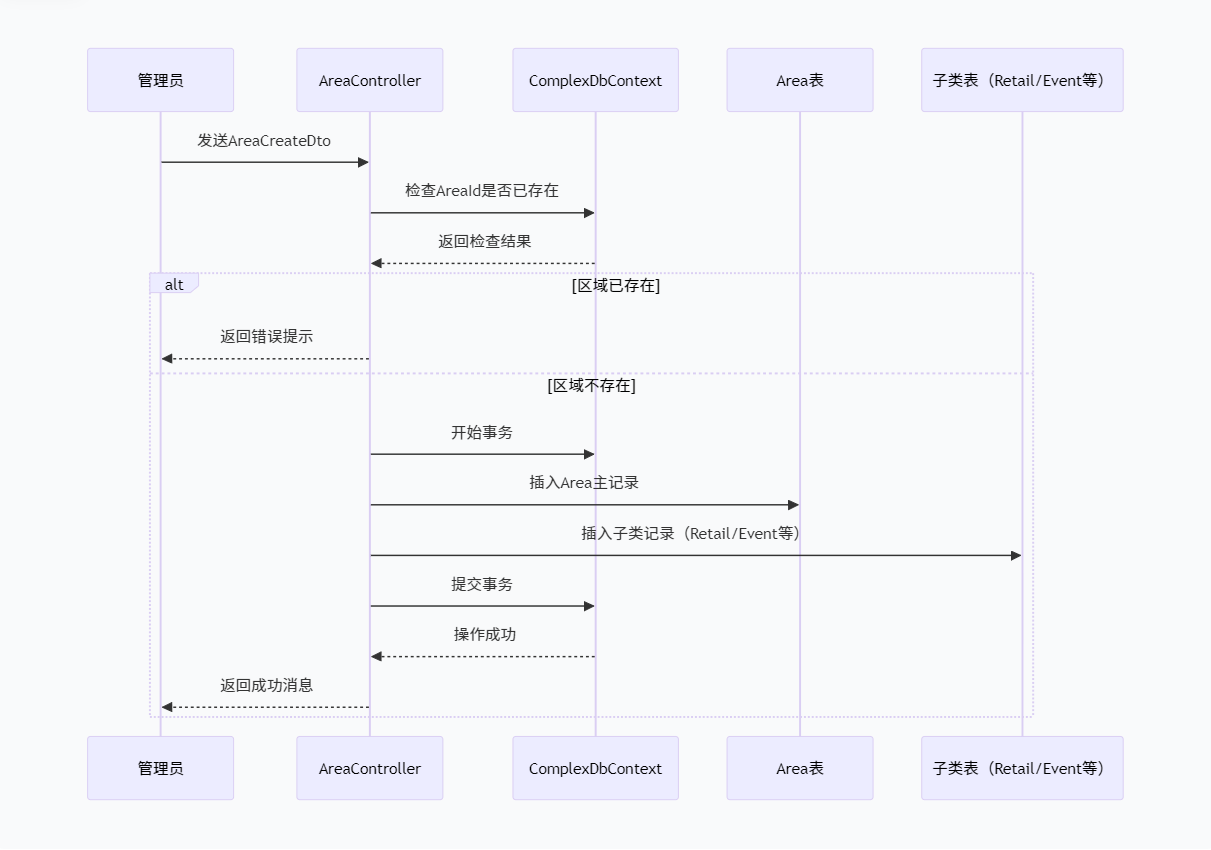
\includegraphics[width=5.64167in,height=2.86458in]{media/media/image_2-3-5.png}

区域信息查询

按类别和空置状态查询:
\begin{verbatim}
[HttpGet("ByCategory")]
public async Task<IActionResult> GetAreas([FromQuery] string? category, [FromQuery] int? isEmpty)
\end{verbatim}
按ID查询:
\begin{verbatim}
[HttpGet("ByID")]
public async Task<IActionResult> GetAreasByID([FromQuery] int id)
\end{verbatim}
用户可根据类别和空置状态查询区域信息。系统返回区域基本信息及其子类特定属性(如租金、容量等)。

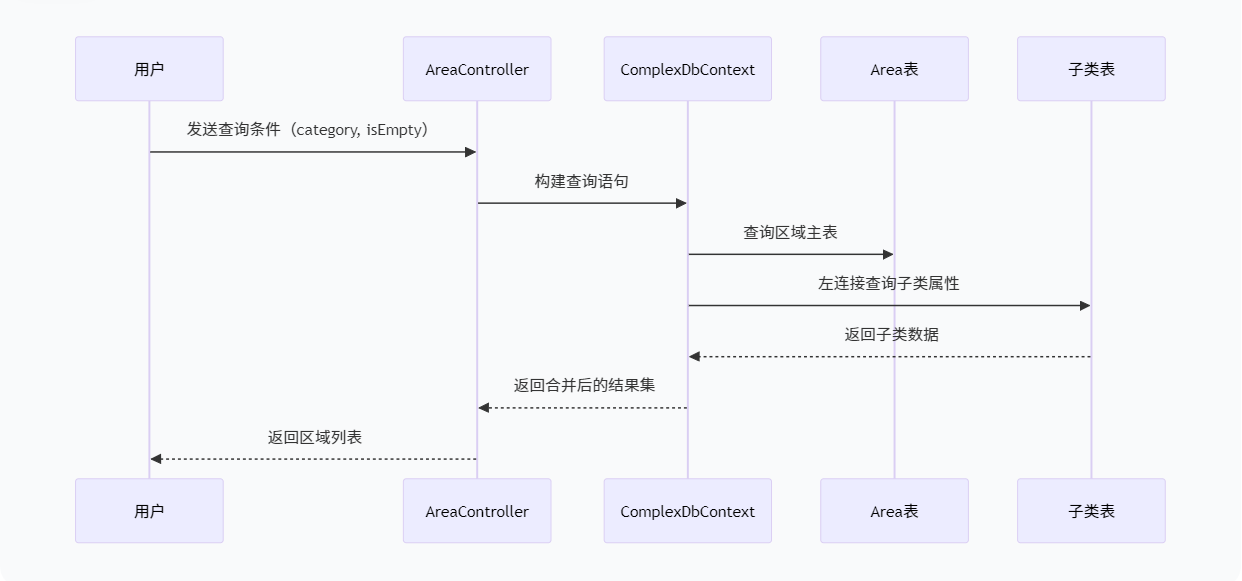
\includegraphics[width=5.64167in,height=2.86458in]{media/media/image_2-3-6.png}

区域信息管理 - 删除

\begin{verbatim}
[HttpDelete("{id}")]
public async Task<IActionResult> DeleteArea(int id)
\end{verbatim}
管理员删除指定区域。系统会检查该区域是否被租用或有关联活动,若无则删除主表和子表记录。

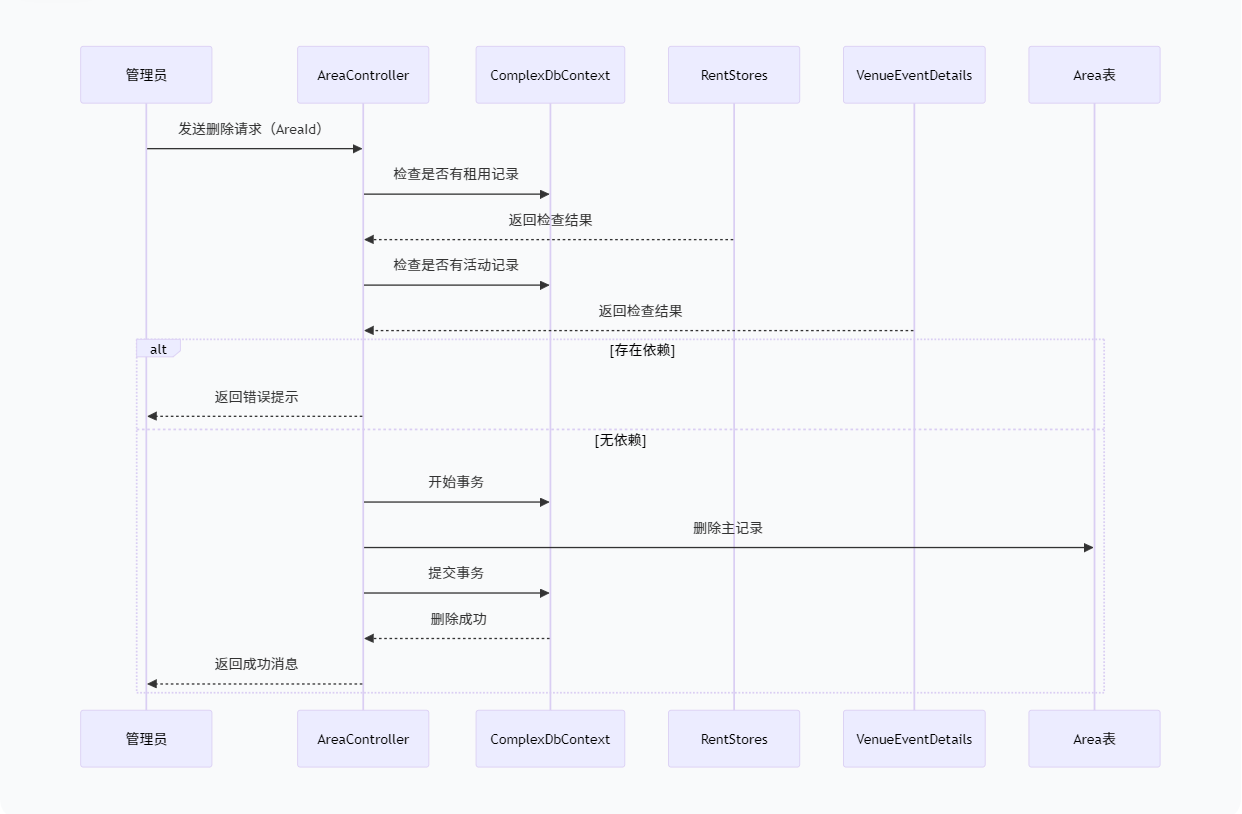
\includegraphics[width=5.64167in,height=2.86458in]{media/media/image_2-3-7.png}

\hypertarget{ux7528ux4f8b-2}{%
  \subsection{合作方用例}\label{ux7528ux4f8b-2}}

\hypertarget{ux7528ux4f8b-2ux8bbeux8ba1}{%
  \subsubsection{合作方用例设计}\label{ux7528ux4f8b-2ux8bbeux8ba1}}

\begin{longtable}[]{@{}ll@{}}
  \toprule
  \textbf{动作序列} & \textbf{描述}                  \\
  \midrule
  \endhead
  添加新合作方        & 在系统内新增一条合作方记录,用于后续场地活动或合作事项  \\
  合作方信息查询       & 项目经理查询合作方的详细信息,用于活动筹备或合作事项跟进 \\
  合作方信息修改       & 项目经理更新合作方的基础信息及关联活动状态        \\
  合作方统计信息报表     & 按时间段生成合作方运营统计报表,支持筛选与导出      \\
  \bottomrule
\end{longtable}

添加新合作方:

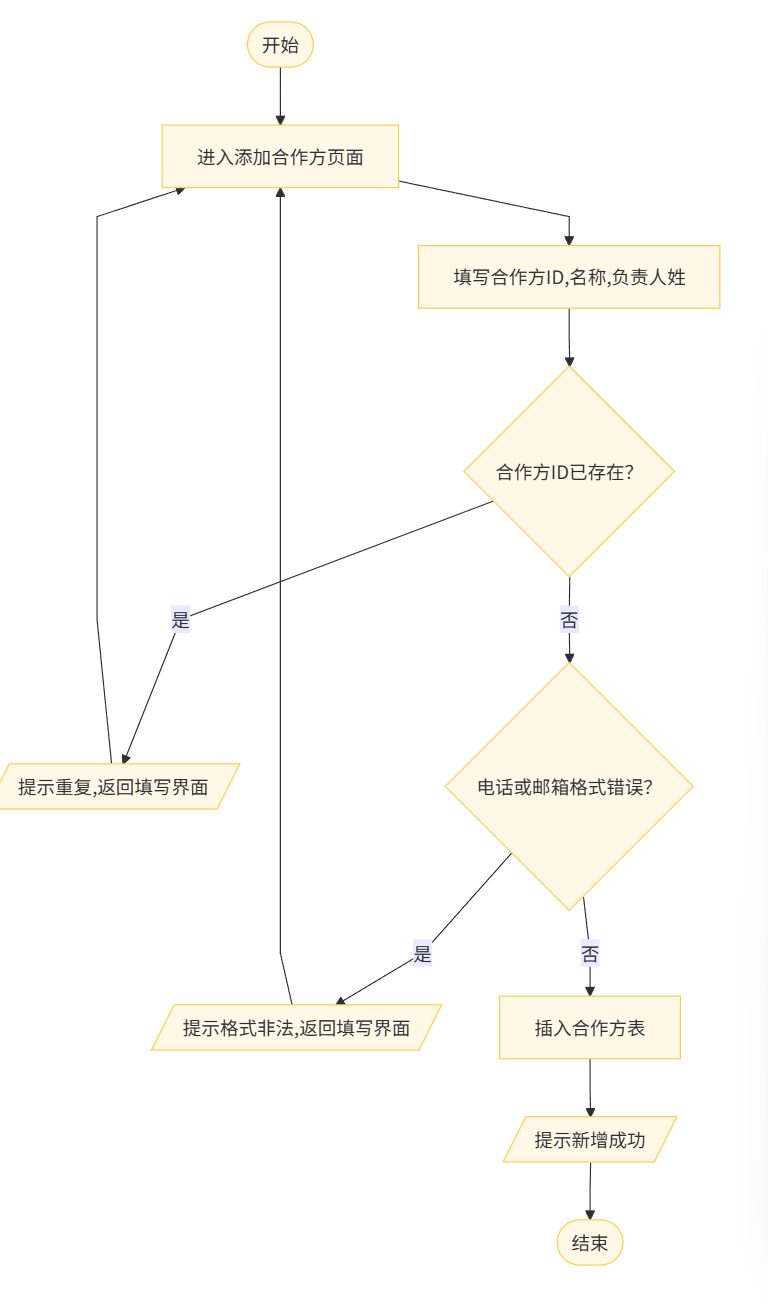
\includegraphics[width=4.45694in,height=4.83819in]{media/media/image_2-4-1.png}

合作方信息查询:

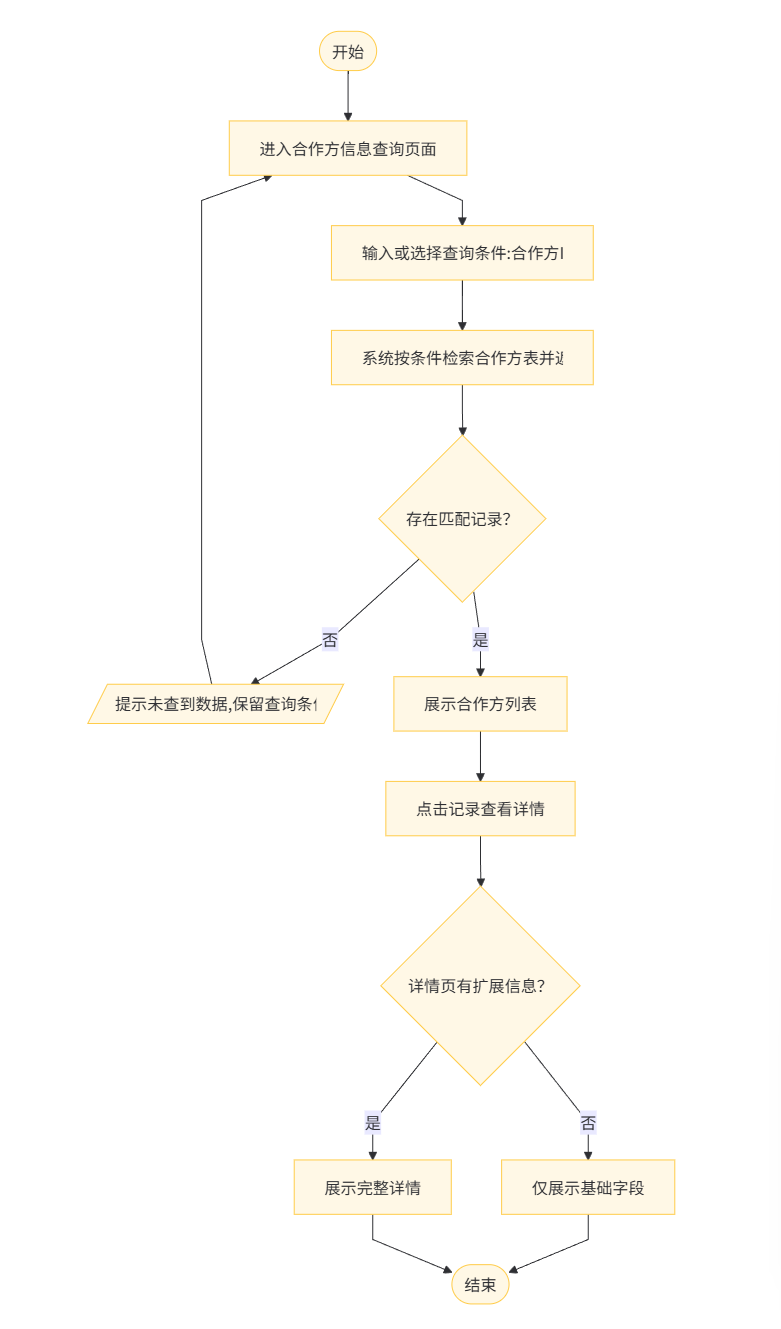
\includegraphics[width=4.45694in,height=4.83819in]{media/media/image_2-4-2.png}

合作方信息修改:

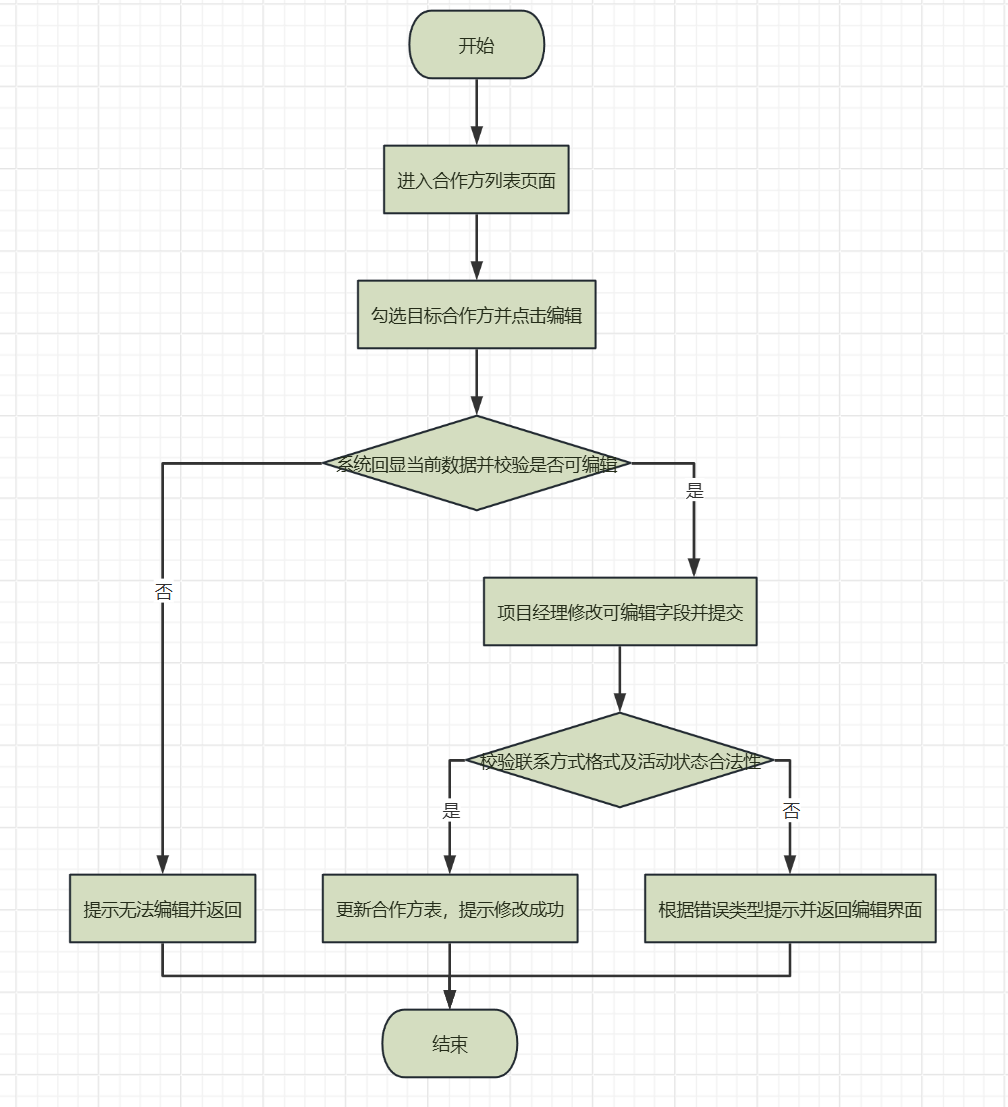
\includegraphics[width=4.45694in,height=4.83819in]{media/media/image_2-4-3.png}

合作方统计信息报表:

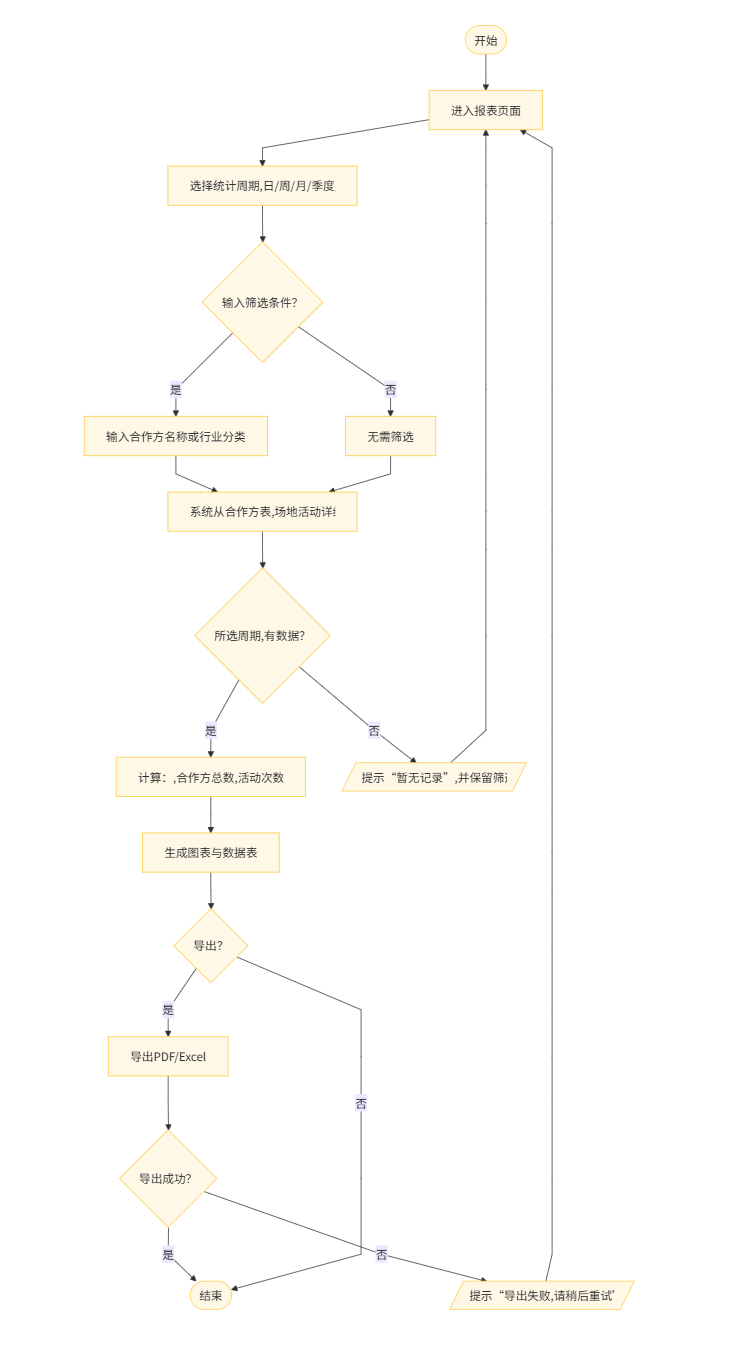
\includegraphics[width=4.45694in,height=4.83819in]{media/media/image_2-4-4.png}


\hypertarget{ux7528ux4f8b-2ux5b9eux73b0}{%
  \subsubsection{合作方用例实现}\label{ux7528ux4f8b-2ux5b9eux73b0}}

合作方用例实现

添加新合作方:

\begin{verbatim}
public class CollaborationDto
{
    [Required(ErrorMessage = "合作方ID是必填项")]
    [Range(1, 99999999999, ErrorMessage = "合作方ID必须大于0,且不能超过11位")]
    public int CollaborationId { get; set; }

    [Required(ErrorMessage = "合作方名称是必填项")]
    [StringLength(50, ErrorMessage = "名称长度不能超过50个字符")]
    public string CollaborationName { get; set; }

    [StringLength(50, ErrorMessage = "联系人姓名长度不能超过50个字符")]
    public string Contactor { get; set; }

    [Phone(ErrorMessage = "无效的电话号码格式")]
    [StringLength(20, ErrorMessage = "电话号码长度不能超过20个字符")]
    public string PhoneNumber { get; set; }

    [EmailAddress(ErrorMessage = "无效的电子邮件格式")]
    [StringLength(50, ErrorMessage = "电子邮件长度不能超过50个字符")]
    public string Email { get; set; }
}
[HttpPost]
public async Task<IActionResult> AddCollaboration(
    [FromQuery, Required] string operatorAccountId,
    [FromBody] CollaborationDto dto)
\end{verbatim}

首先验证操作员是否具有数据库管理员权限(1),然后检查提供的合作方ID是否已存在。如果ID唯一,则创建新的合作方实体并保存到数据库,同时记录操作日志。用于系统管理员添加新的合作方信息,确保合作方数据的唯一性和完整性,为后续的场馆活动合作提供基础数据支持。

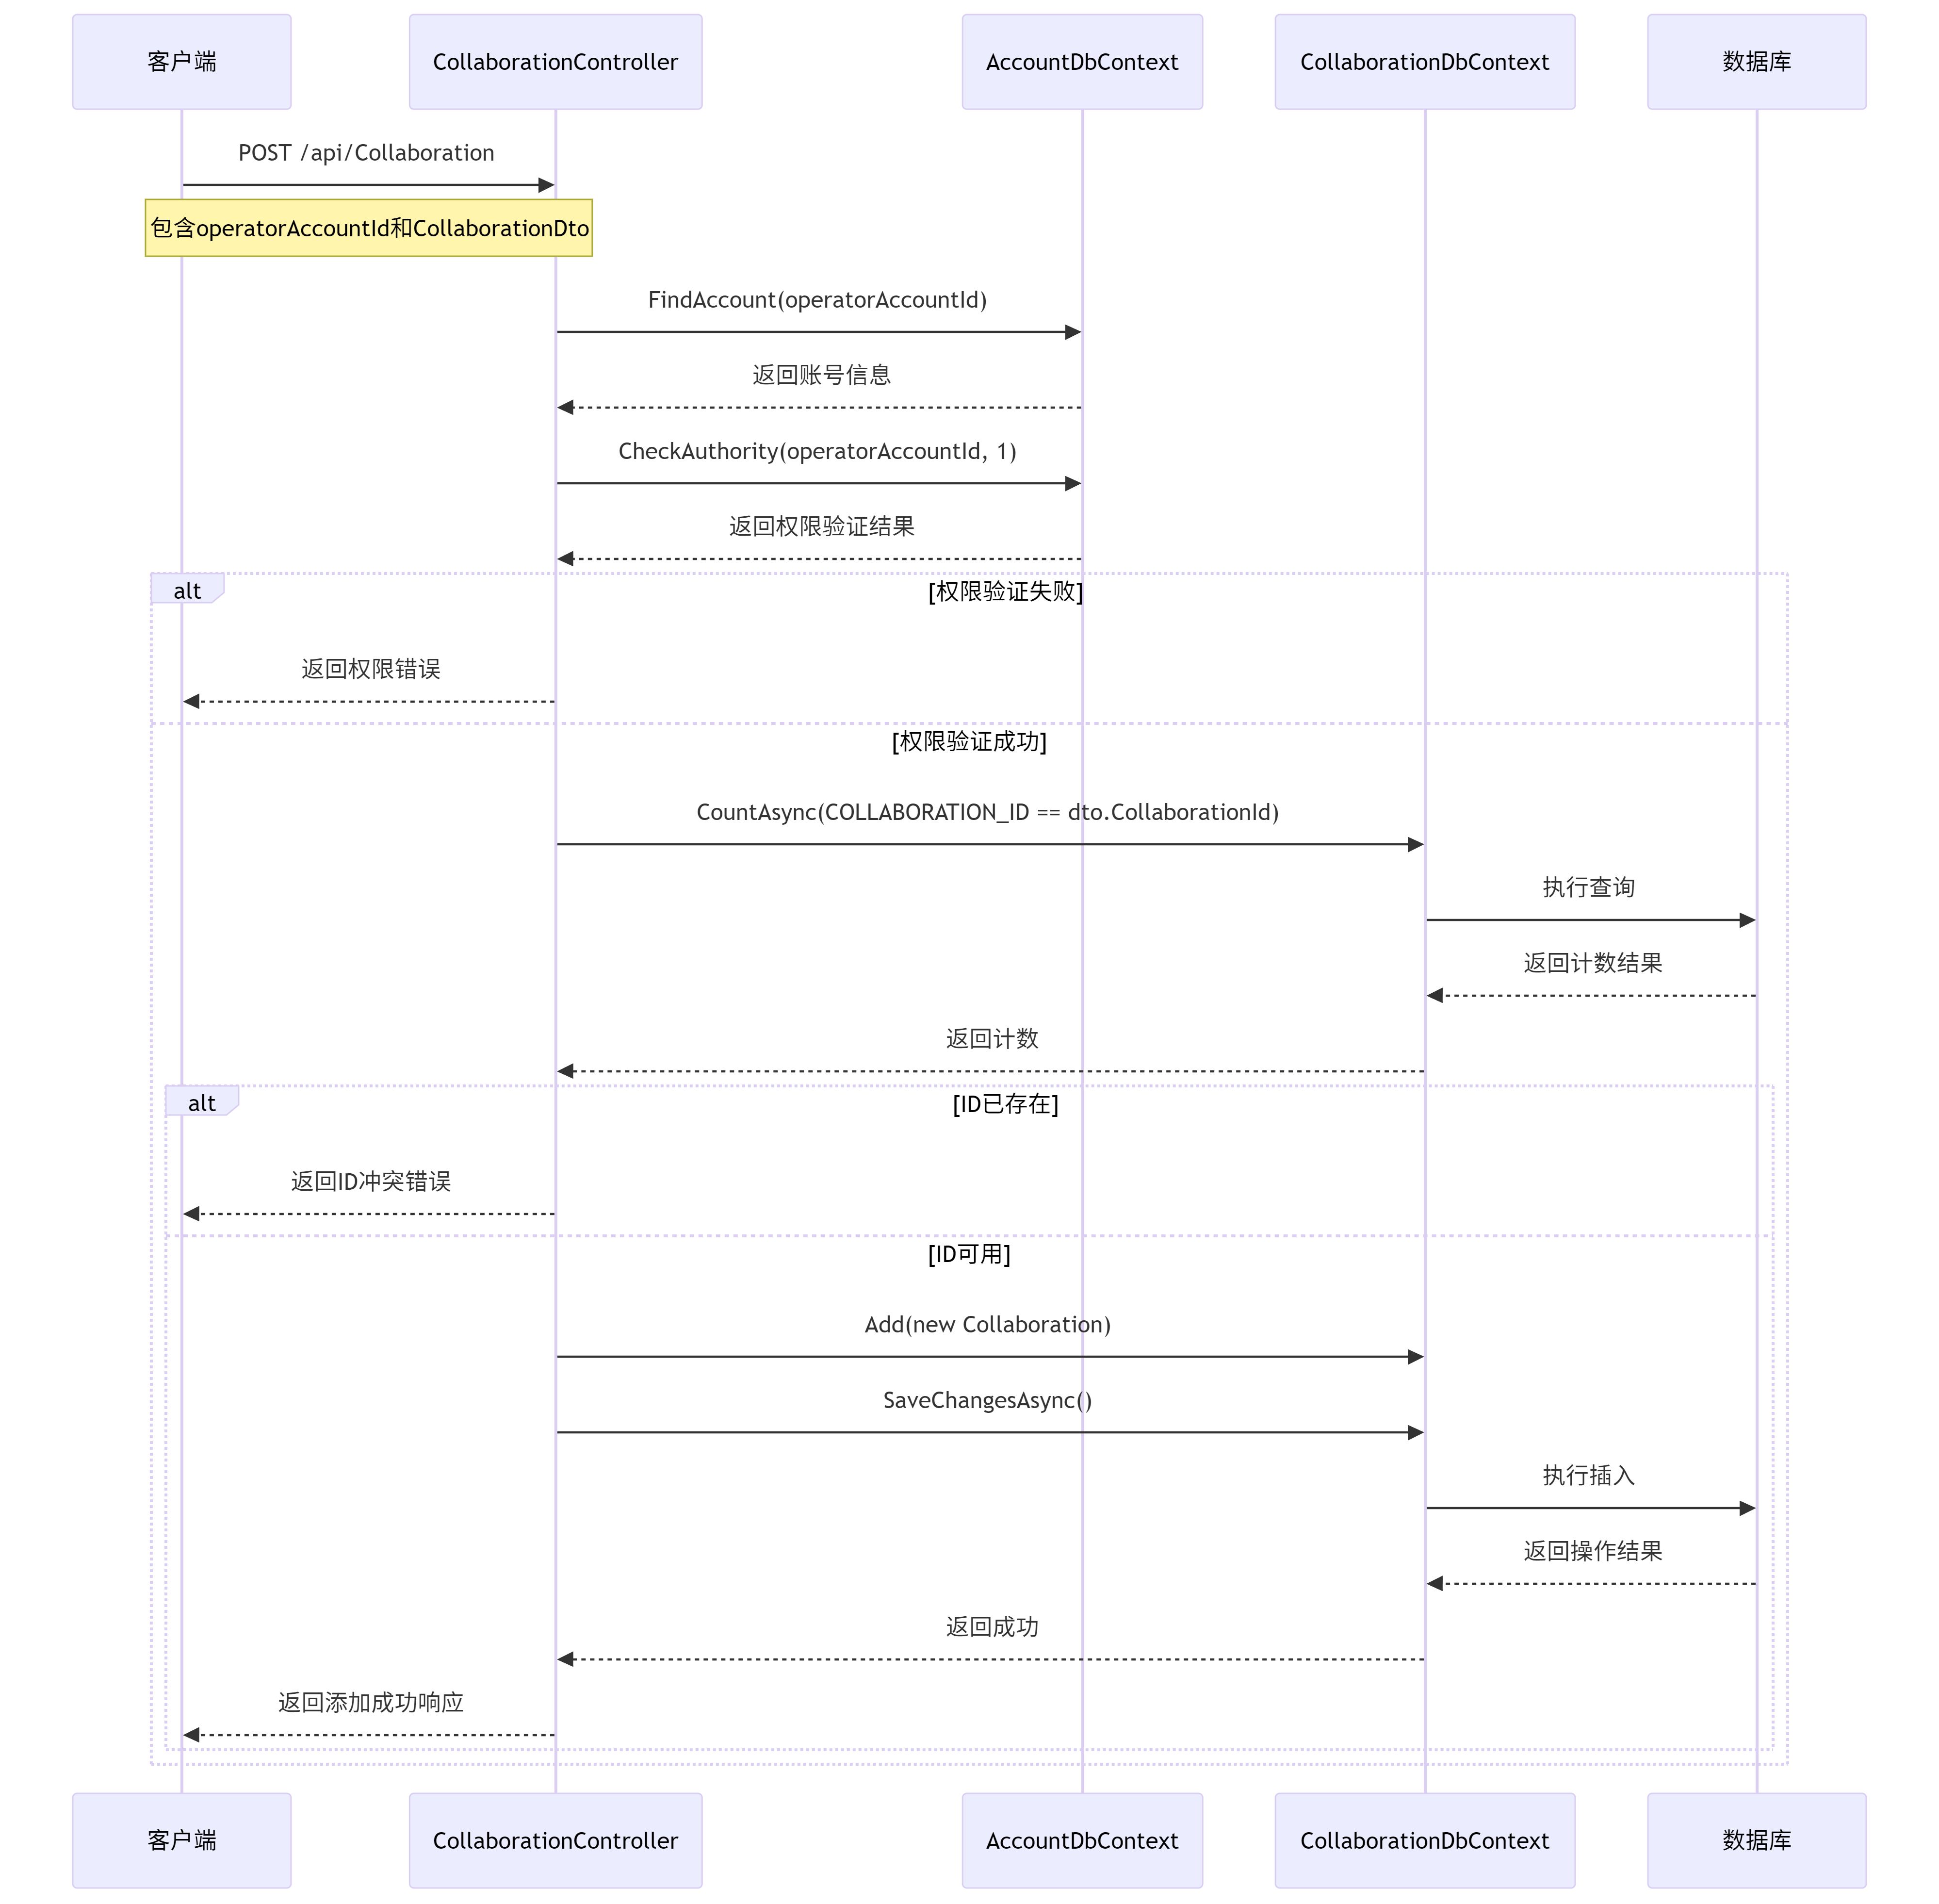
\includegraphics[width=5.64167in,height=2.86458in]{media/media/image_2-4-5.png}

合作方信息查询:

\begin{verbatim}
[HttpGet]
public async Task<IActionResult> SearchCollaborations(
    [FromQuery, Required] string operatorAccountId,
    [FromQuery] int? id,
    [FromQuery] string? name,
    [FromQuery] string? contactor)
\end{verbatim}

验证操作员是否具有数据库管理员(1)或部门经理权限(2),然后根据提供的查询条件(ID、名称或联系人)构建动态查询,返回匹配的合作方列表。为管理人员提供灵活的合作方信息检索功能,支持按多种条件筛选,便于快速查找特定合作方信息。

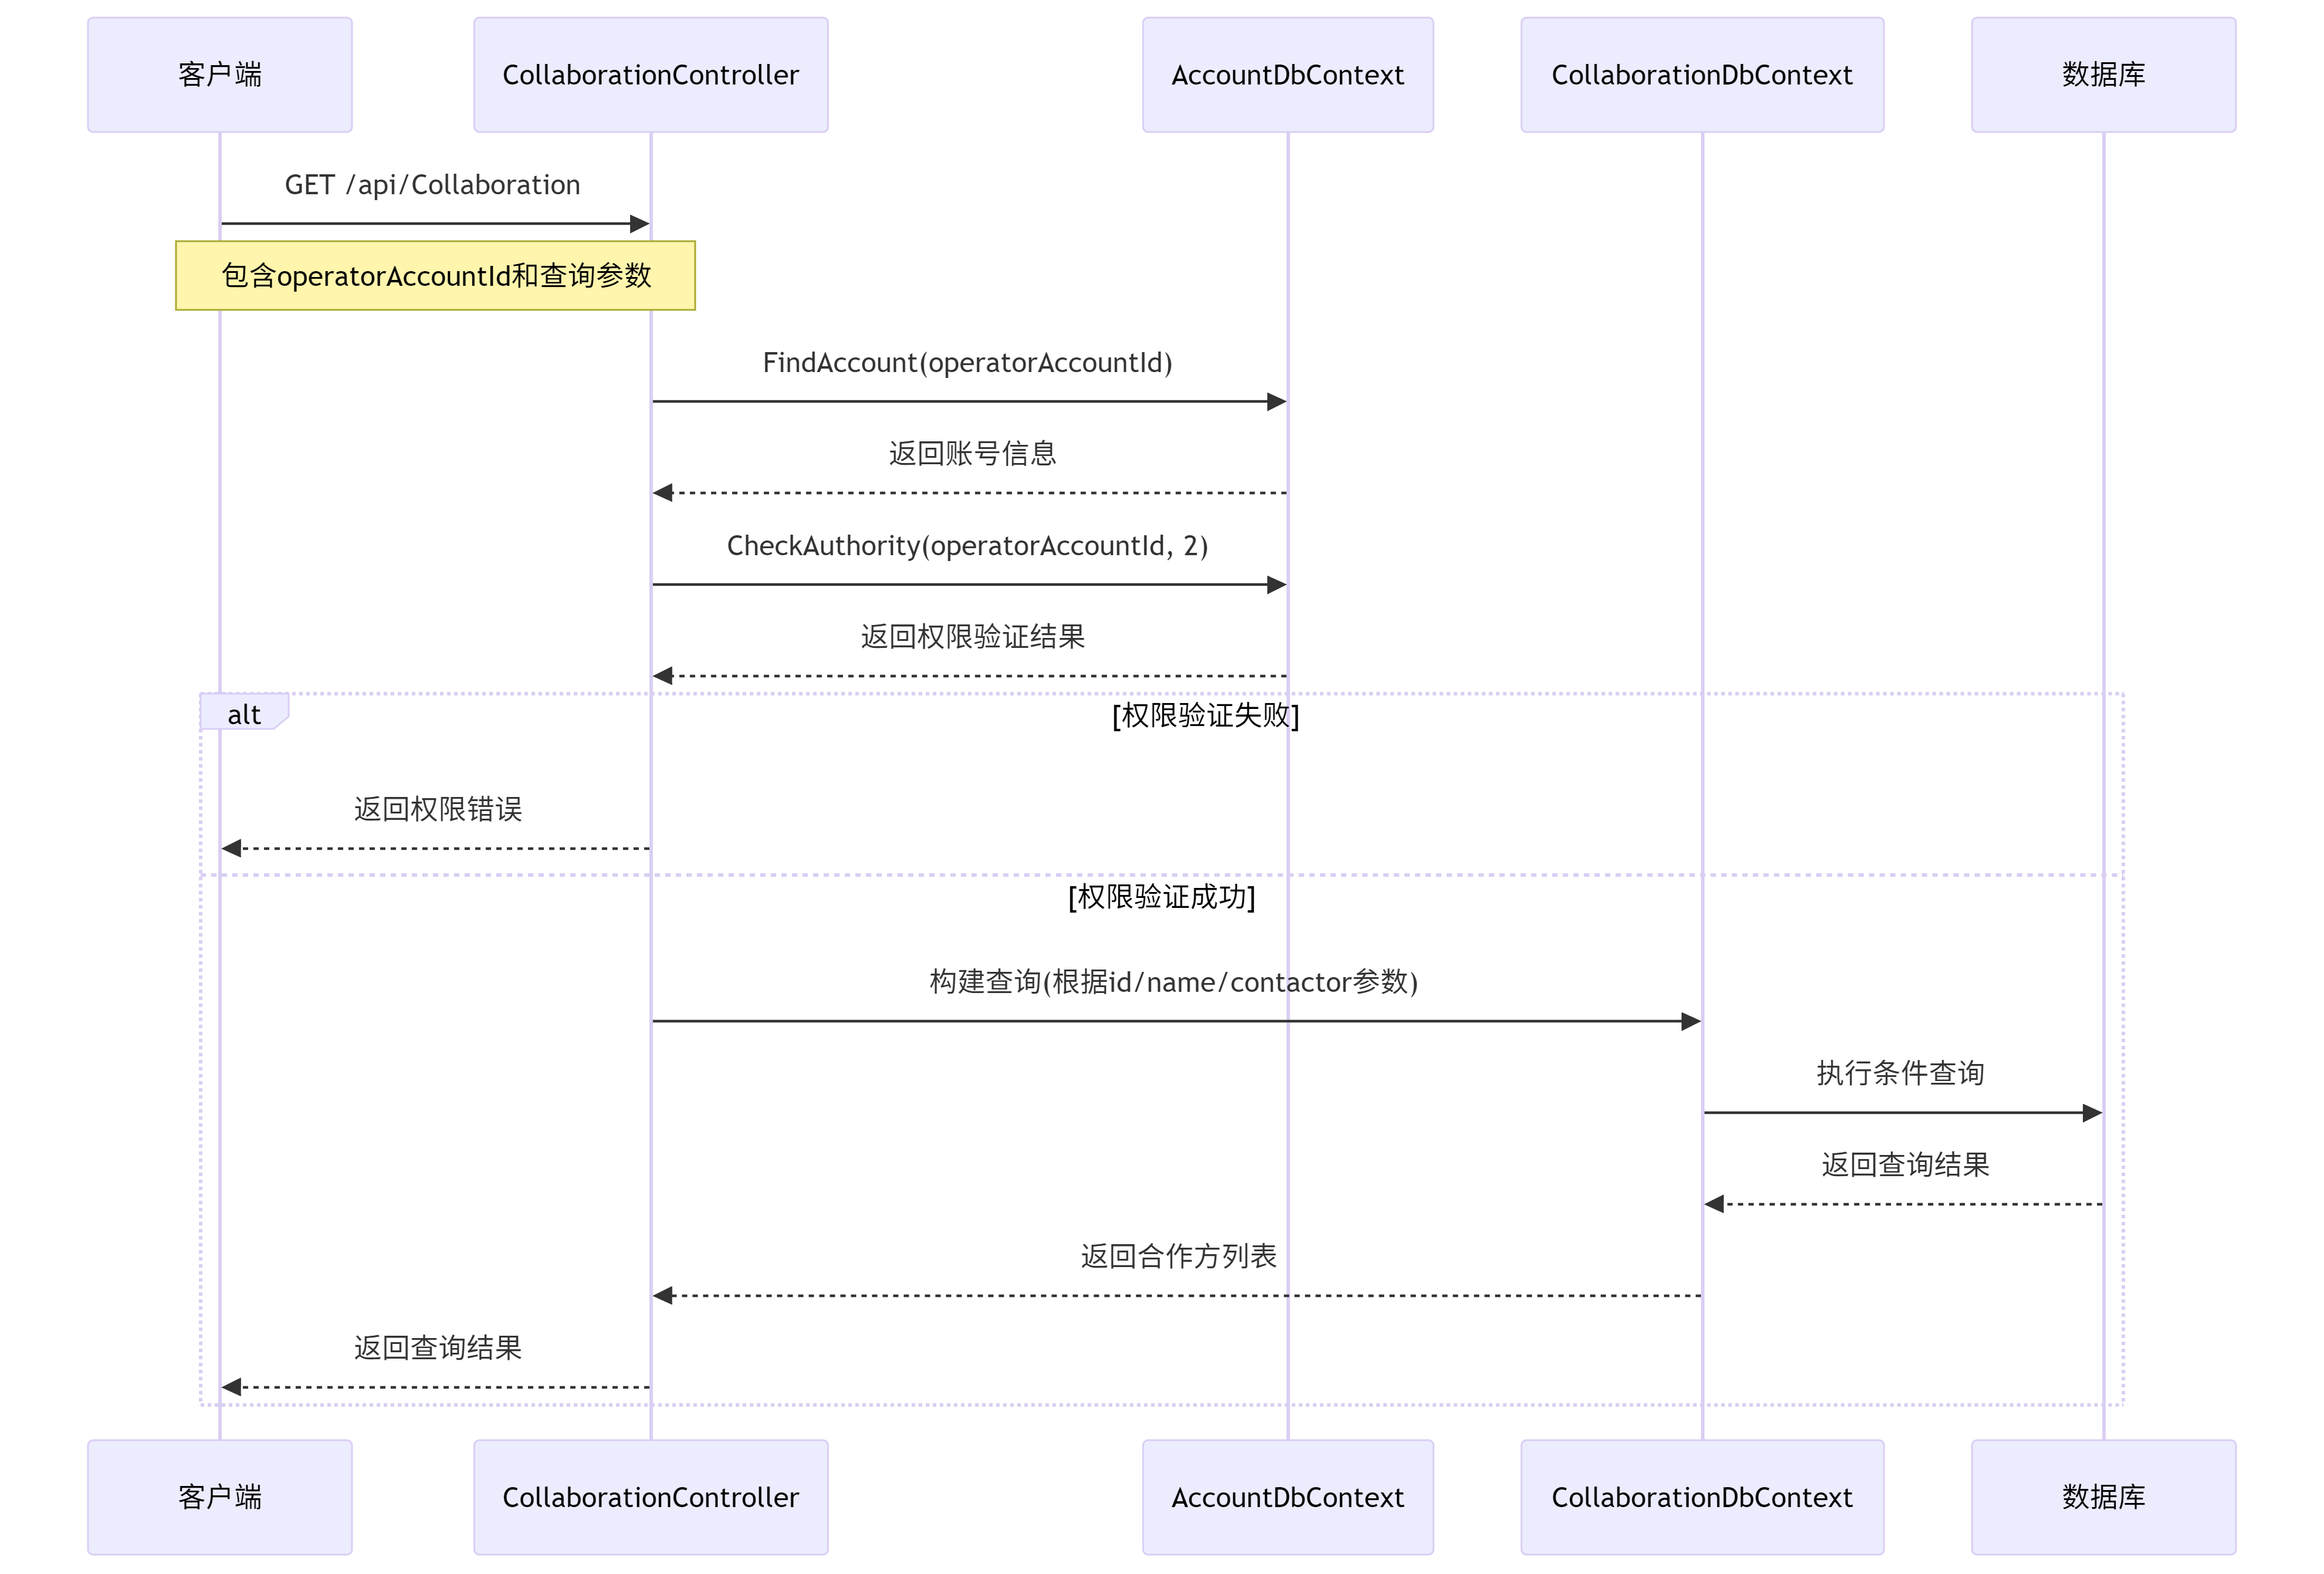
\includegraphics[width=5.64167in,height=2.86458in]{media/media/image_2-4-6.png}

合作方信息修改:

\begin{verbatim}
public class CollaborationUpdateDto
{
    [StringLength(50, ErrorMessage = "名称长度不能超过50个字符")]
    public string CollaborationName { get; set; }

    [StringLength(50, ErrorMessage = "联系人姓名长度不能超过50个字符")]
    public string Contactor { get; set; }

    [Phone(ErrorMessage = "无效的电话号码格式")]
    [StringLength(20, ErrorMessage = "电话号码长度不能超过20个字符")]
    public string PhoneNumber { get; set; }

    [EmailAddress(ErrorMessage = "无效的电子邮件格式")]
    [StringLength(50, ErrorMessage = "电子邮件长度不能超过50个字符")]
    public string Email { get; set; }
}
[HttpPut("{id}")]
public async Task<IActionResult> UpdateCollaboration(
    int id, 
    [FromQuery, Required] string operatorAccountId,
    [FromBody] CollaborationUpdateDto dto)
\end{verbatim}

验证操作员是否具有数据库管理员权限(1),检查目标合作方是否存在以及是否正在进行活动(存在活动则不允许修改)。若可修改,则更新合作方的可修改字段并保存更改。允许系统管理员维护合作方信息的准确性,确保合作方数据的时效性,同时防止对正在进行活动的合作方造成干扰。

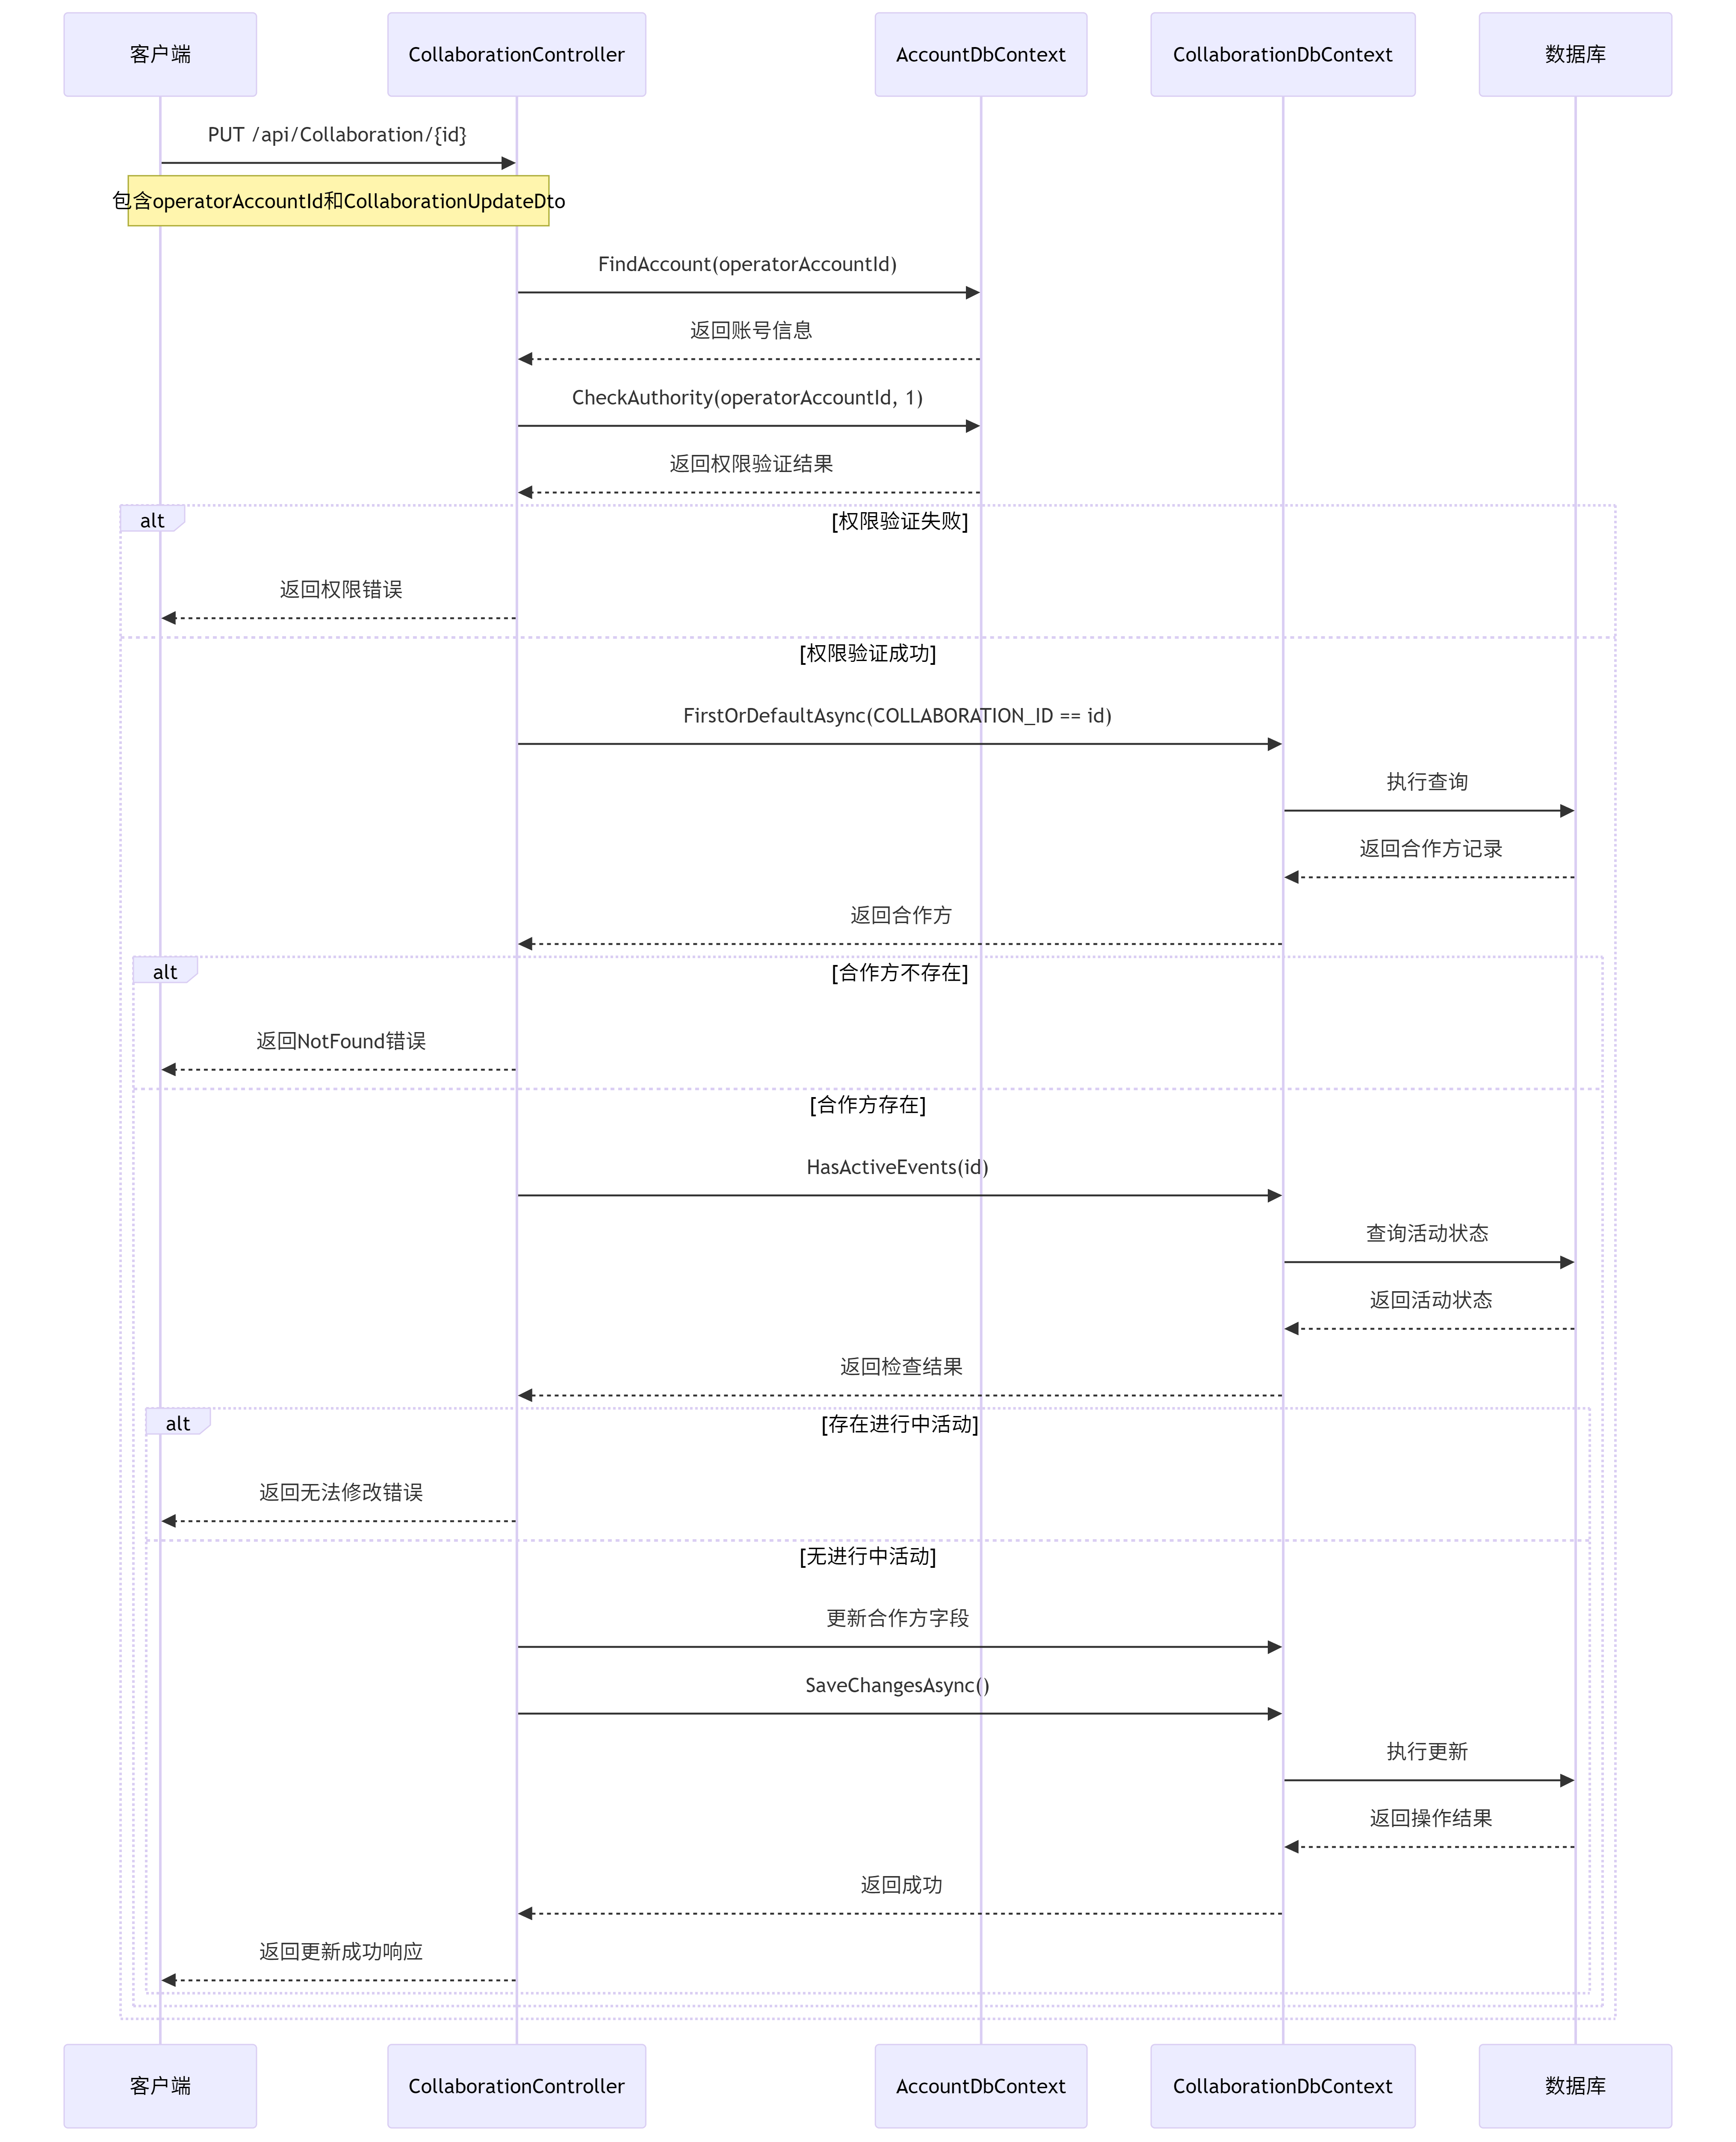
\includegraphics[width=5.64167in,height=2.86458in]{media/media/image_2-4-7.png}

合作方统计信息报表:

\begin{verbatim}
[HttpGet("report")]
public async Task<IActionResult> GenerateReport(
    [FromQuery, Required] string operatorAccountId,
    [FromQuery] DateTime startDate,
    [FromQuery] DateTime endDate,
    [FromQuery] string? industry)
\end{verbatim}

验证操作员权限(需要权限1或2),验证时间范围的合理性,然后按时间范围和行业筛选条件统计各合作方的活动数量、总投资和平均收益。为管理层提供合作方业务活动的统计分析数据,支持决策制定,帮助评估不同合作方的贡献度和投资回报率

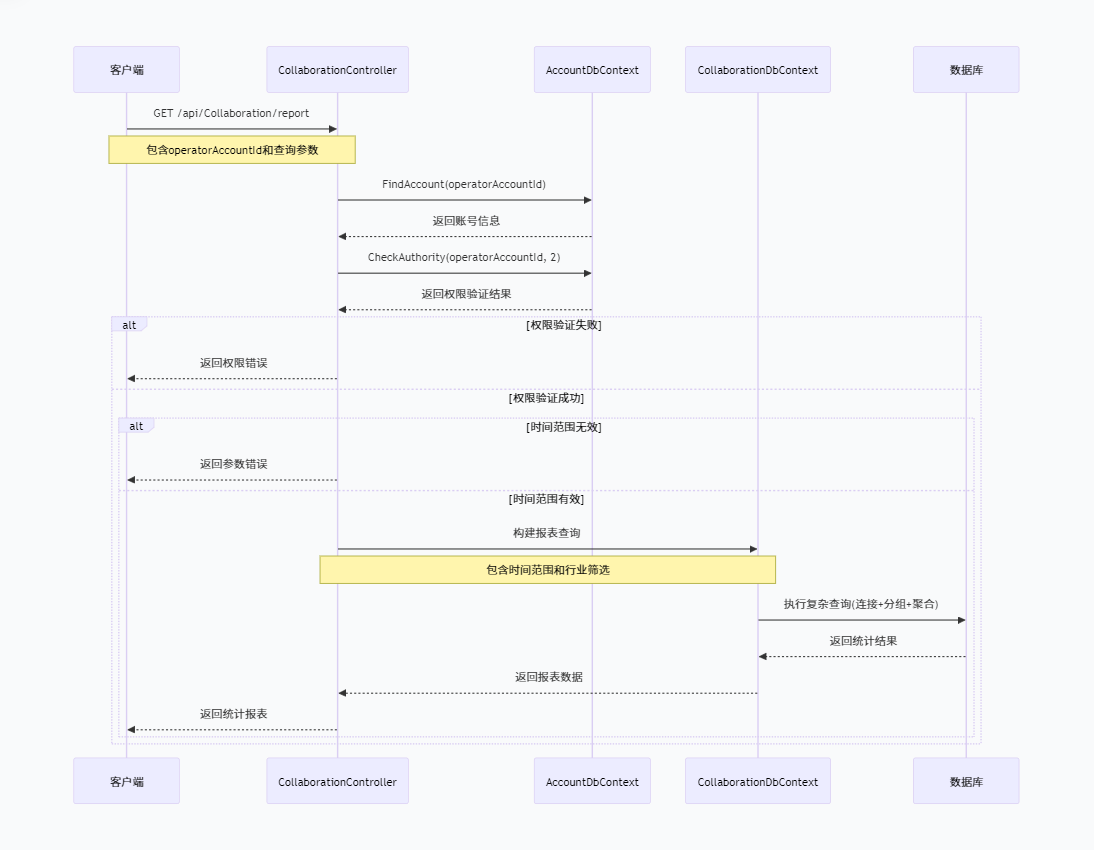
\includegraphics[width=5.64167in,height=2.86458in]{media/media/image_2-4-8.png}

\hypertarget{ux7528ux4f8b-3}{%
  \subsection{**用例}\label{ux7528ux4f8b-3}}

\hypertarget{ux5458ux5de5ux7528ux4f8b}{%
  \subsection{员工用例}\label{ux5458ux5de5ux7528ux4f8b}}

\hypertarget{ux5458ux5de5ux7528ux4f8bux8bbeux8ba1}{%
  \subsubsection{员工用例设计}\label{ux5458ux5de5ux7528ux4f8bux8bbeux8ba1}}

表格 2‑6 员工功能的动作序列

\begin{longtable}[]{@{}ll@{}}
  \toprule
  动作序列         & 描述\tabularnewline
  \midrule
  \endhead
  添加新员工        & 管理员创建员工账号并分配基础权限。\tabularnewline
  员工权限管理       & 管理人员调整员工的长期权限\tabularnewline
  员工个人信息修改     &
  员工修改个人可编辑信息,管理人员可修改下属的更多信息\tabularnewline
  员工工资管理       & 对员工工资进行管理\tabularnewline
  员工工资统计报表生成功能 &
  系统按部门、时间等维度生成员工工资统计报表\tabularnewline
  员工临时权限管理     & 为员工授予 /
  收回与特定活动相关的临时权限\tabularnewline
  \bottomrule
\end{longtable}

添加员工活动图:

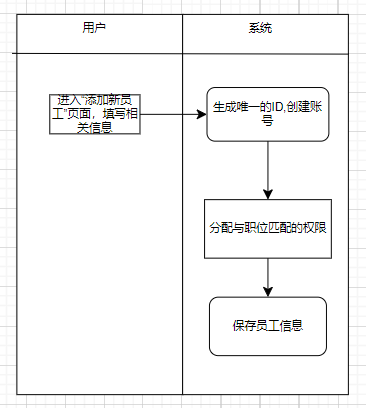
\includegraphics[width=3.10417in,height=3.45694in]{media/media/image8.png}

员工权限管理活动图:

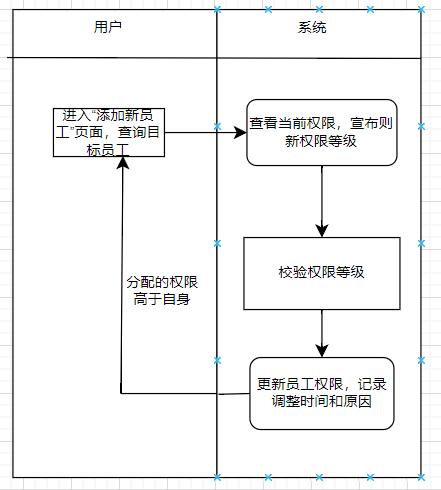
\includegraphics[width=2.95972in,height=3.28333in]{media/media/image9.png}

员工个人信息修改活动图:

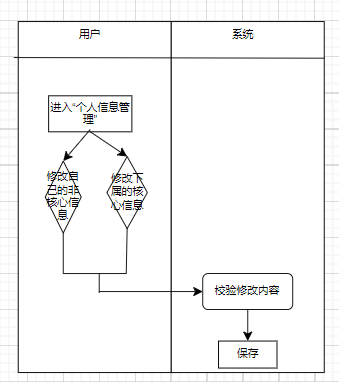
\includegraphics[width=3.53194in,height=3.98264in]{media/media/image10.png}

员工工资管理活动图:

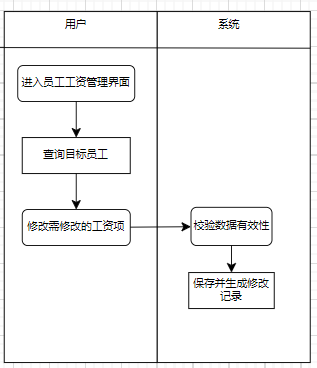
\includegraphics[width=3.02917in,height=3.51458in]{media/media/image11.png}

员工工资统计报表生成活动图:

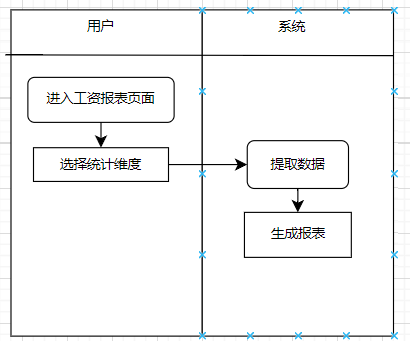
\includegraphics[width=2.90764in,height=2.41597in]{media/media/image12.png}

员工临时权限管理活动图:

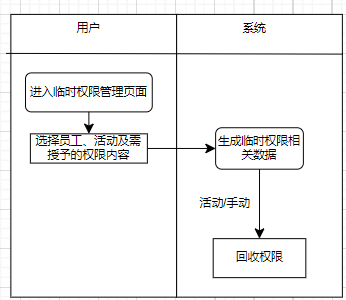
\includegraphics[width=3.075in,height=2.66458in]{media/media/image13.png}

\hypertarget{ux5458ux5de5ux7528ux4f8bux5b9eux73b0}{%
  \subsubsection{员工用例实现}\label{ux5458ux5de5ux7528ux4f8bux5b9eux73b0}}

1. 主要类及其关系:

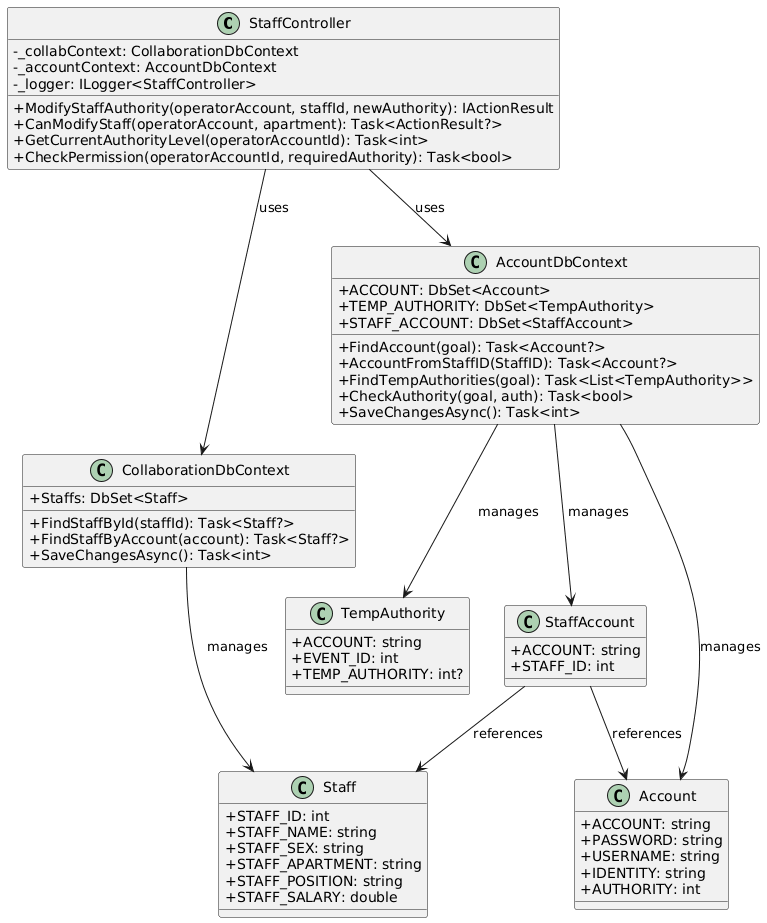
\includegraphics[width=6.23958in,height=7.50903in]{media/media/image14.png}

2. 方法设计与实现:

添加员工:
\begin{verbatim}
public class StaffDto
{
    [Required(ErrorMessage = "员工姓名是必填项")]
    [StringLength(50, ErrorMessage = "名称长度不能超过50个字符")]
    public string STAFF_NAME { get; set; }
    [StringLength(10, ErrorMessage = "性别长度不能超过10个字符")]
    public string STAFF_SEX { get; set; }
    [Required(ErrorMessage = "员工部门是必填项")]
    [StringLength(50, ErrorMessage = "部门长度不能超过50个字符")]
    public string STAFF_APARTMENT { get; set; }
    [Required(ErrorMessage = "员工职位是必填项")]
    [StringLength(50, ErrorMessage = "职位长度不能超过50个字符")]
    public string STAFF_POSITION { get; set; }
    [Required(ErrorMessage = "员工薪资是必填项")]
    [Range(0, 9999999999.99, ErrorMessage = "薪资必须大于等于0,且不能超过10位整数和2位小数")]
    public double STAFF_SALARY { get; set; }
}

[HttpPost("AddStaff")]
public async Task<IActionResult> AddStaff(
    [FromQuery, Required] string operatorAccount,
    [FromBody] StaffDto dto)
{
\end{verbatim}

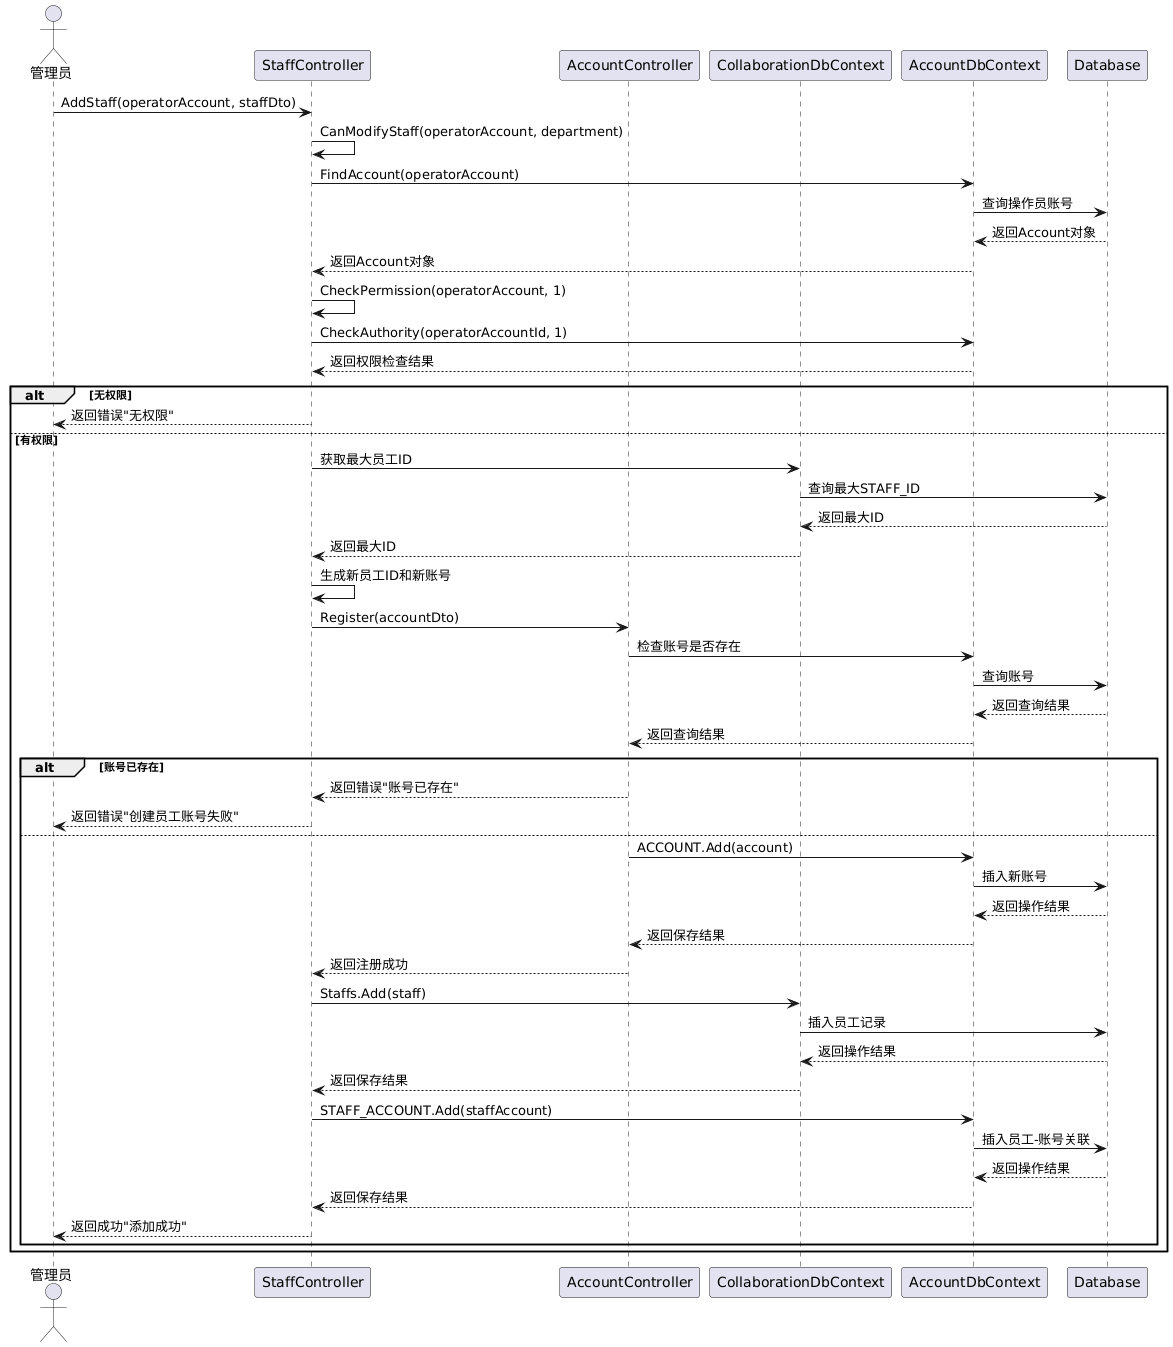
\includegraphics[width=6.27778in,height=7.20903in]{media/media/image15.png}

员工权限管理:
\begin{verbatim}
[HttpPatch("ModifyStaffAuthority")]
public async Task<IActionResult> ModifyStaffAuthority(
    [FromQuery, Required] string operatorAccount,
    [FromQuery] int staffId,
    [FromQuery] int newAuthority)
\end{verbatim}

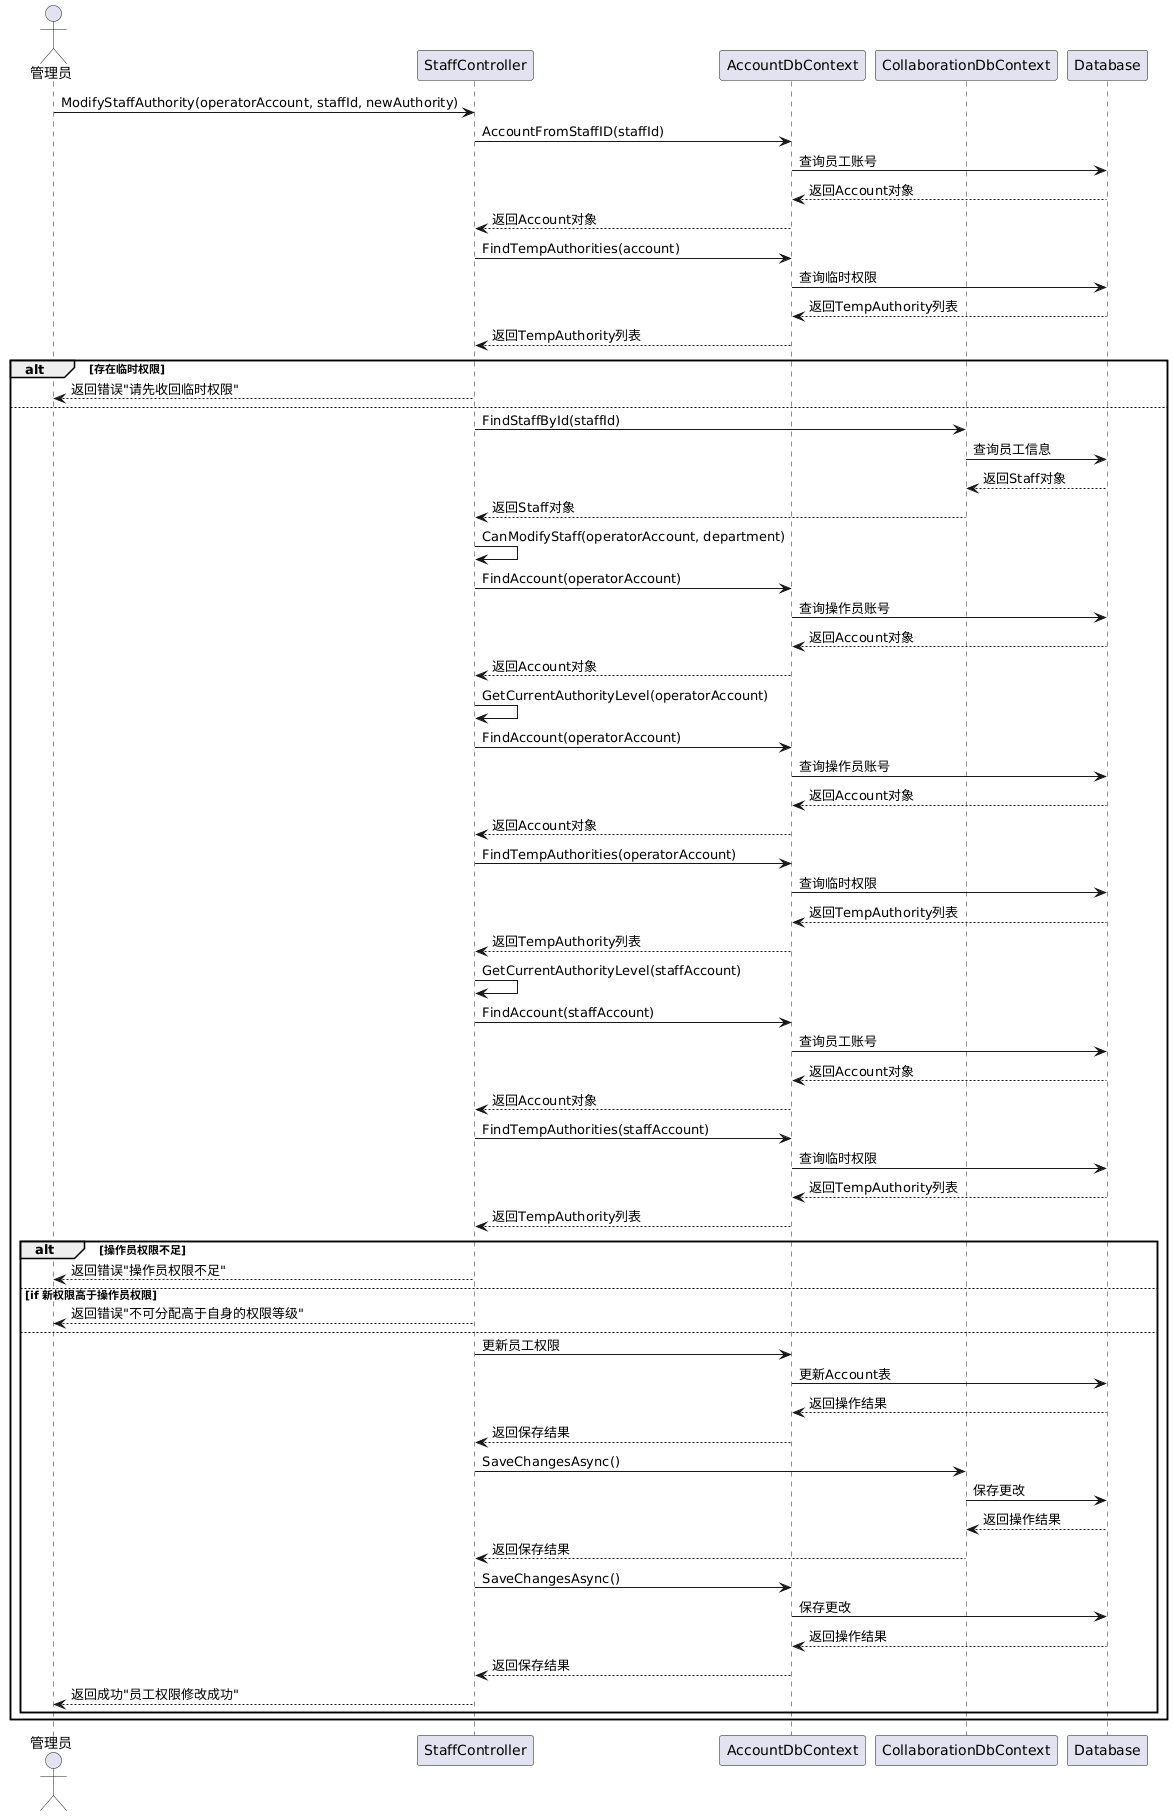
\includegraphics[width=5.98403in,height=9.26389in]{media/media/image16.png}

员工修改信息:
\begin{verbatim}
[HttpPatch("ModifyStaffInfo")]
public async Task<IActionResult> UpdateStaff(
    [FromQuery, Required] int staffId,
    [FromQuery, Required] string operatorAccount,
    [FromBody] StaffDto dto)
\end{verbatim}

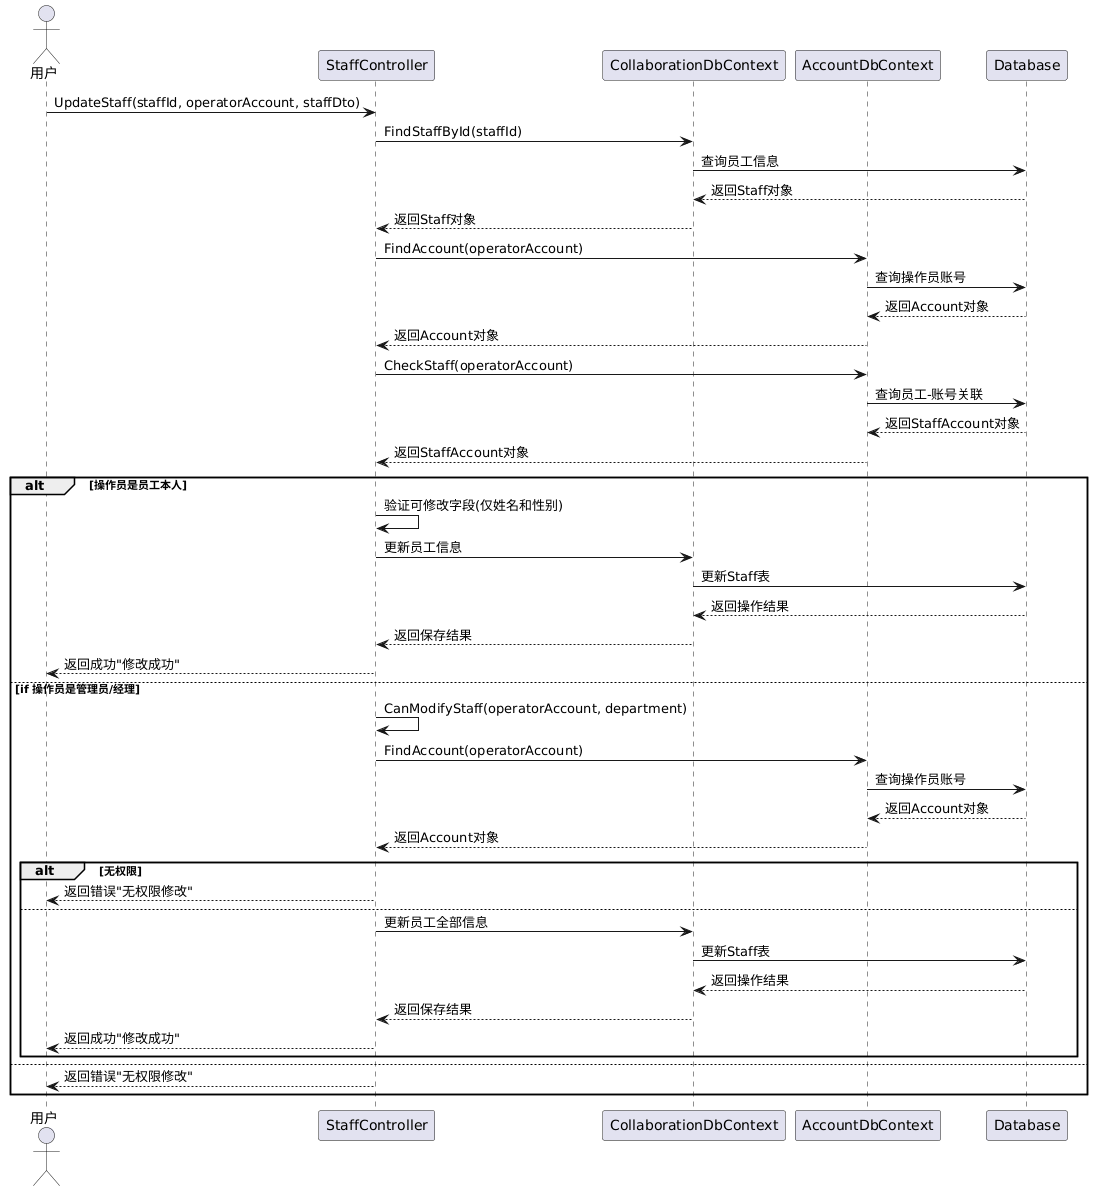
\includegraphics[width=6.20625in,height=6.7625in]{media/media/image17.png}

员工工资管理:
\begin{verbatim}
[HttpPost("StaffSalaryManagement")]
public async Task<IActionResult> ManageStaffSalary(
    [FromQuery, Required] string operatorAccount,
    [FromQuery, Required] int staffId,
    [FromQuery] DateTime monthTime, // 格式 如 2008-11
    [FromBody] SalaryDto dto)
\end{verbatim}

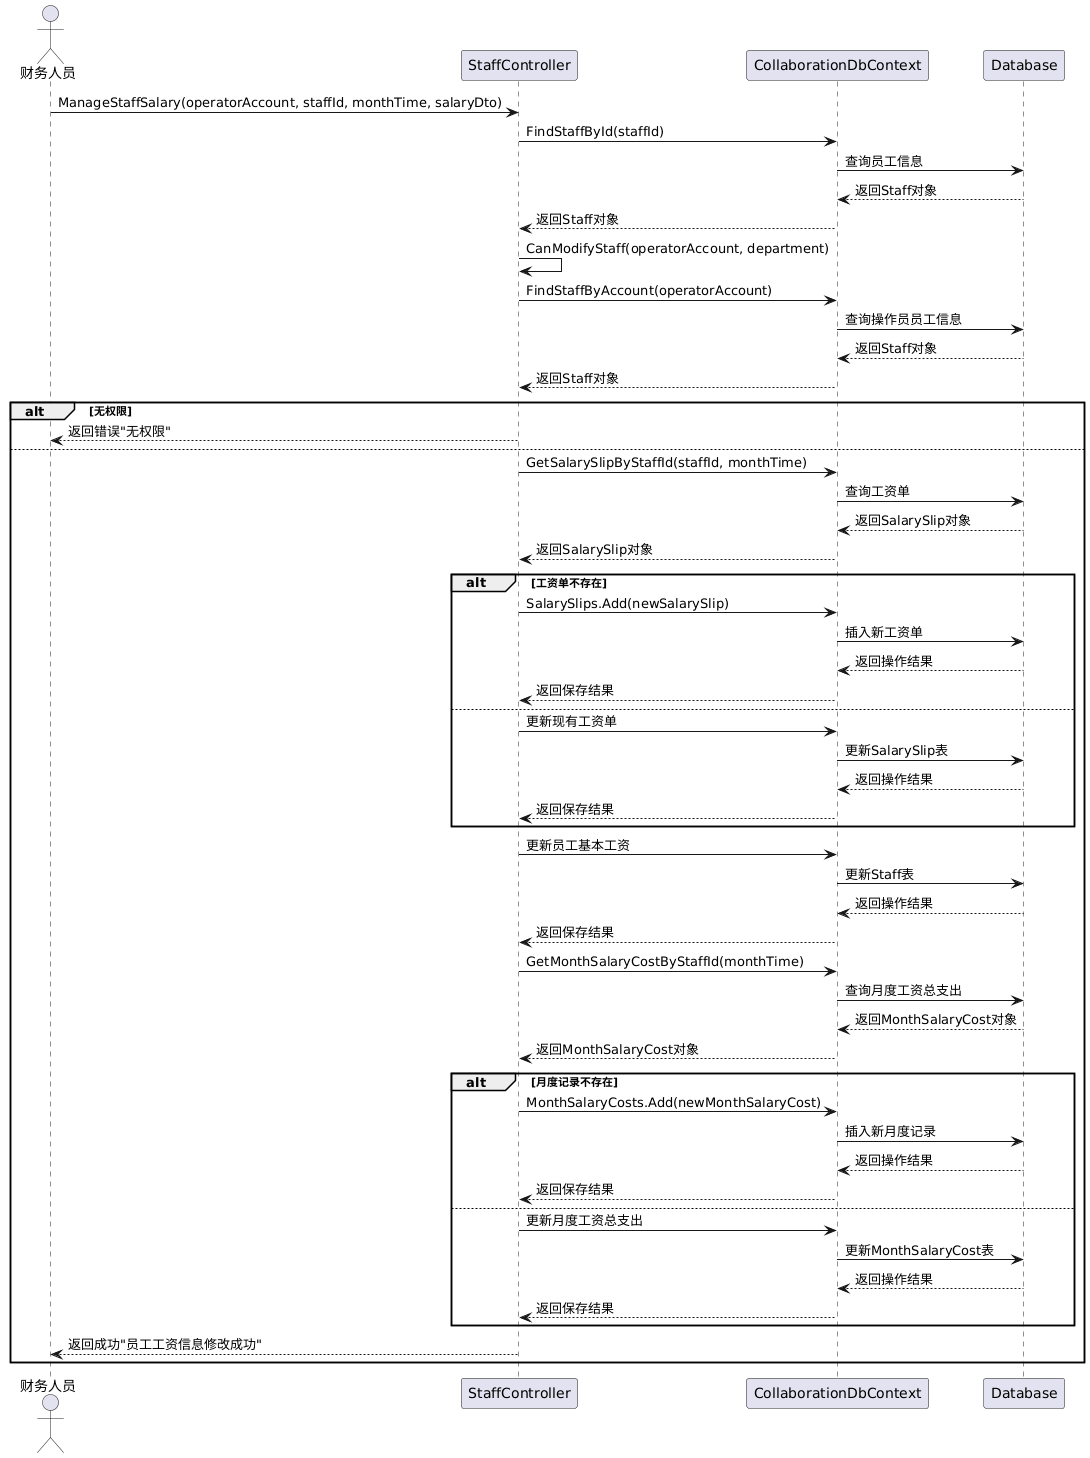
\includegraphics[width=6.32153in,height=8.45556in]{media/media/image18.png}

临时权限管理:
\begin{verbatim}
[HttpPost("temporary_authority")]
public async Task<IActionResult> ManageTemporaryAuthority(
    [FromQuery, Required] string operatorAccount,
    [FromBody, Required] TempAuthorityDto dto)

[HttpDelete("revoke_temporary_authority")]
public async Task<IActionResult> RevokeTemporaryAuthority(
    [FromQuery, Required] string operatorAccount,
    [FromQuery, Required] string staffAccount,
    [FromQuery, Required] int eventId)
\end{verbatim}

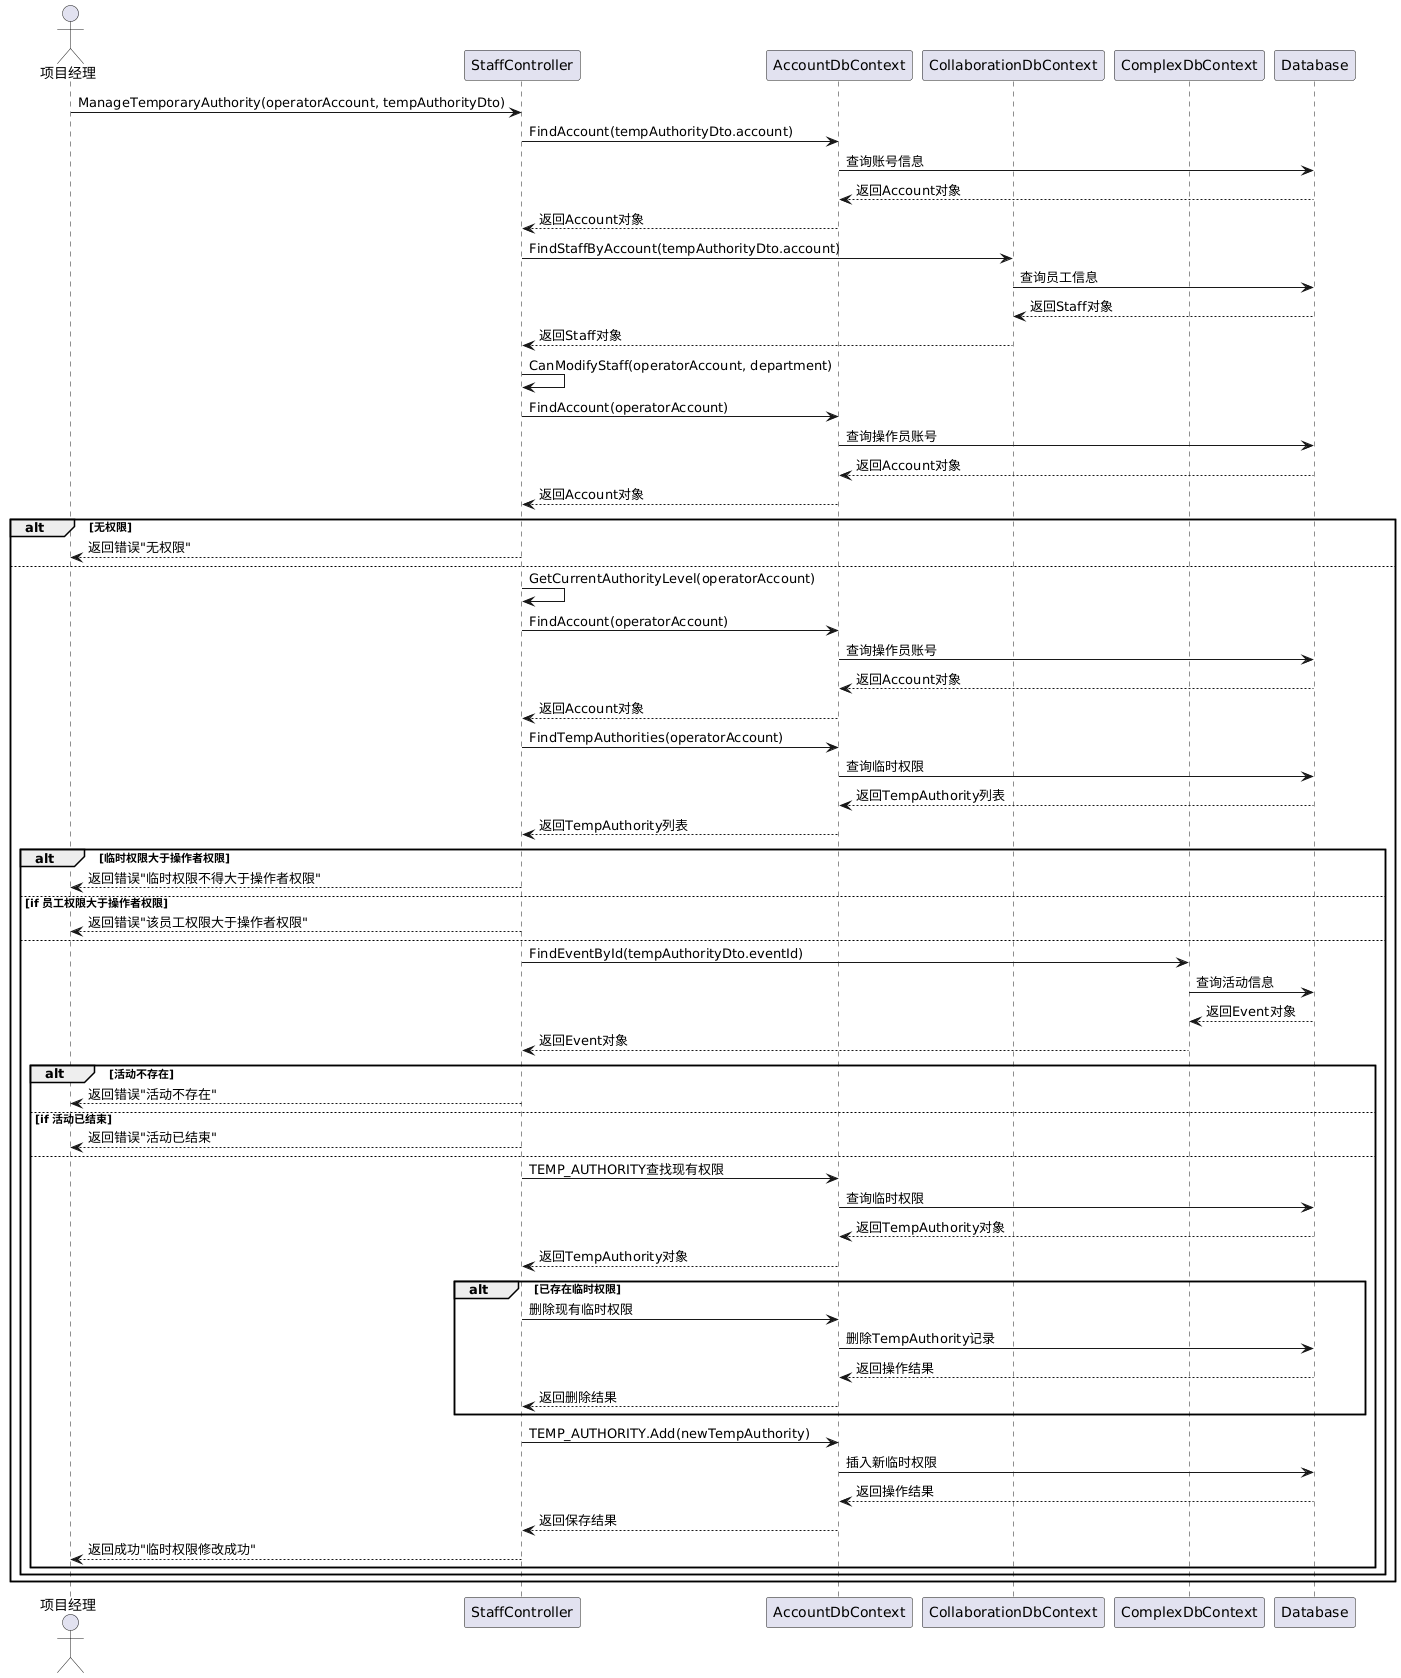
\includegraphics[width=6.28194in,height=7.52361in]{media/media/image19.png}

\hypertarget{ux6d3bux52a8ux7528ux4f8b}{%
\subsection{活动用例}\label{ux6d3bux52a8ux7528ux4f8b}}

\hypertarget{ux6d3bux52a8ux7528ux4f8bux8bbeux8ba1}{%
\subsubsection{活动用例设计}\label{ux6d3bux52a8ux7528ux4f8bux8bbeux8ba1}}

\subsubsection{场地活动}

表格 2-7 场地活动功能的动作序列
\begin{longtable}[]{@{}ll@{}}
\toprule
动作序列 & 描述\tabularnewline
\midrule
\endhead
场地活动预约 & 项目经理提交场地使用申请,由管理员审批,通过后锁定场地资源。\tabularnewline
场地活动管理 & 管理员或项目经理修改已预约活动的信息,如时间、参与人员等,或取消活动。\tabularnewline
场地活动结算收费 & 活动结束后,系统自动计算费用,由项目经理完成结算。\tabularnewline
场地活动统计报表生成 & 系统按多维度生成场地使用率、收入等统计报表。\tabularnewline
\bottomrule
\end{longtable}

场地活动预约活动图:
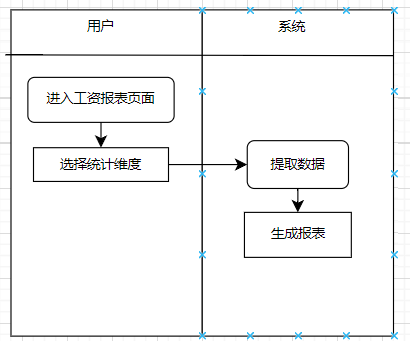
\includegraphics{media/media/image12.png}

场地活动管理活动图:
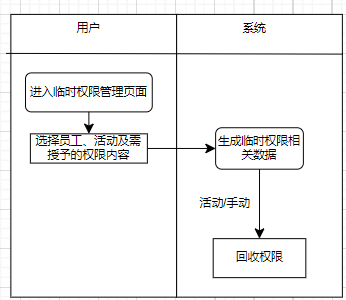
\includegraphics{media/media/image13.png}

场地活动结算收费活动图:
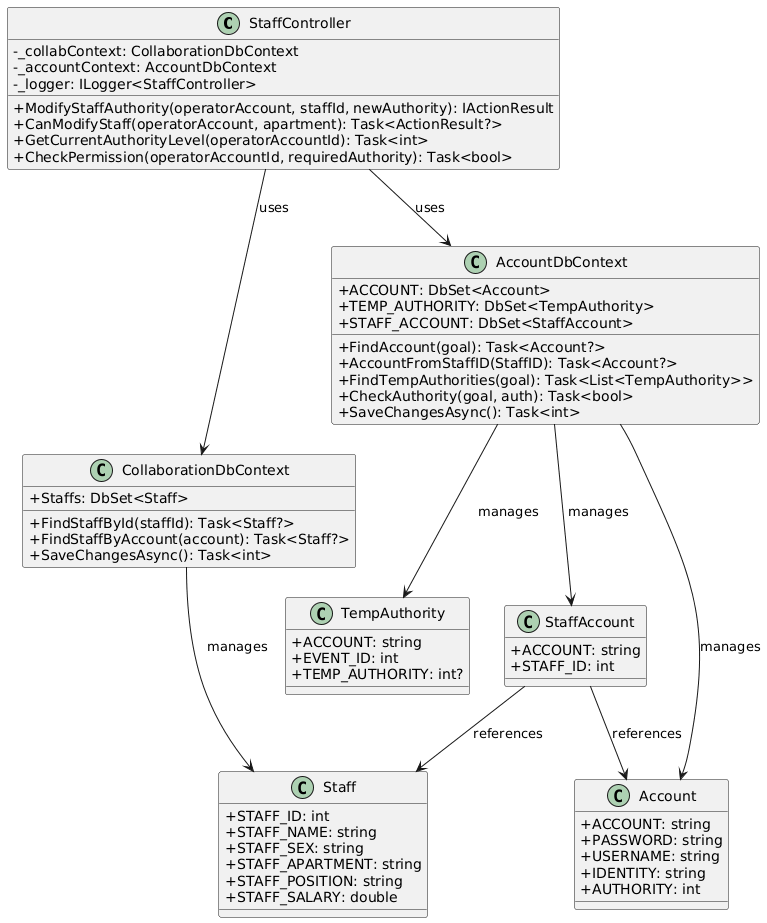
\includegraphics{media/media/image14.png}

场地活动统计报表生成活动图:
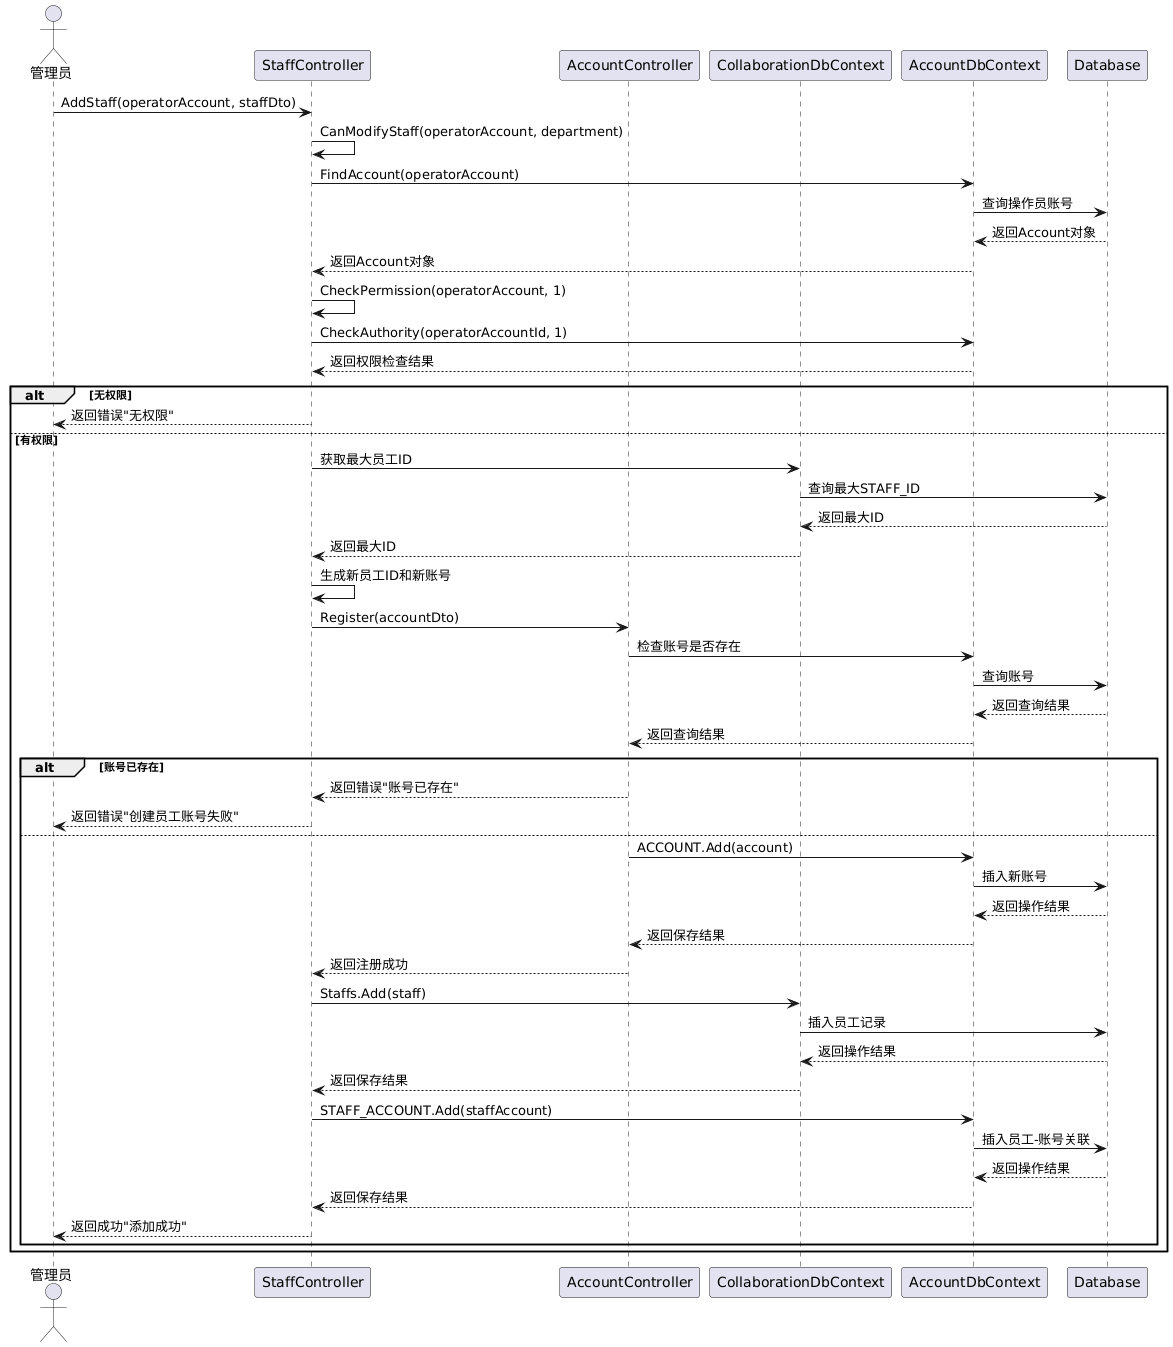
\includegraphics{media/media/image15.png}

\subsubsection{促销活动}

表格 2-8 促销活动功能的动作序列
\begin{longtable}[]{@{}ll@{}}
\toprule
动作序列 & 描述\tabularnewline
\midrule
\endhead
新增促销活动 & 市场专员创建促销活动,设定预算及适用店铺范围。\tabularnewline
促销活动管理 & 管理员监控、调整或终止进行中的促销活动。\tabularnewline
促销活动统计报表生成 & 系统根据指定条件生成促销活动效果的统计报表。\tabularnewline
\bottomrule
\end{longtable}

新增促销活动活动图:
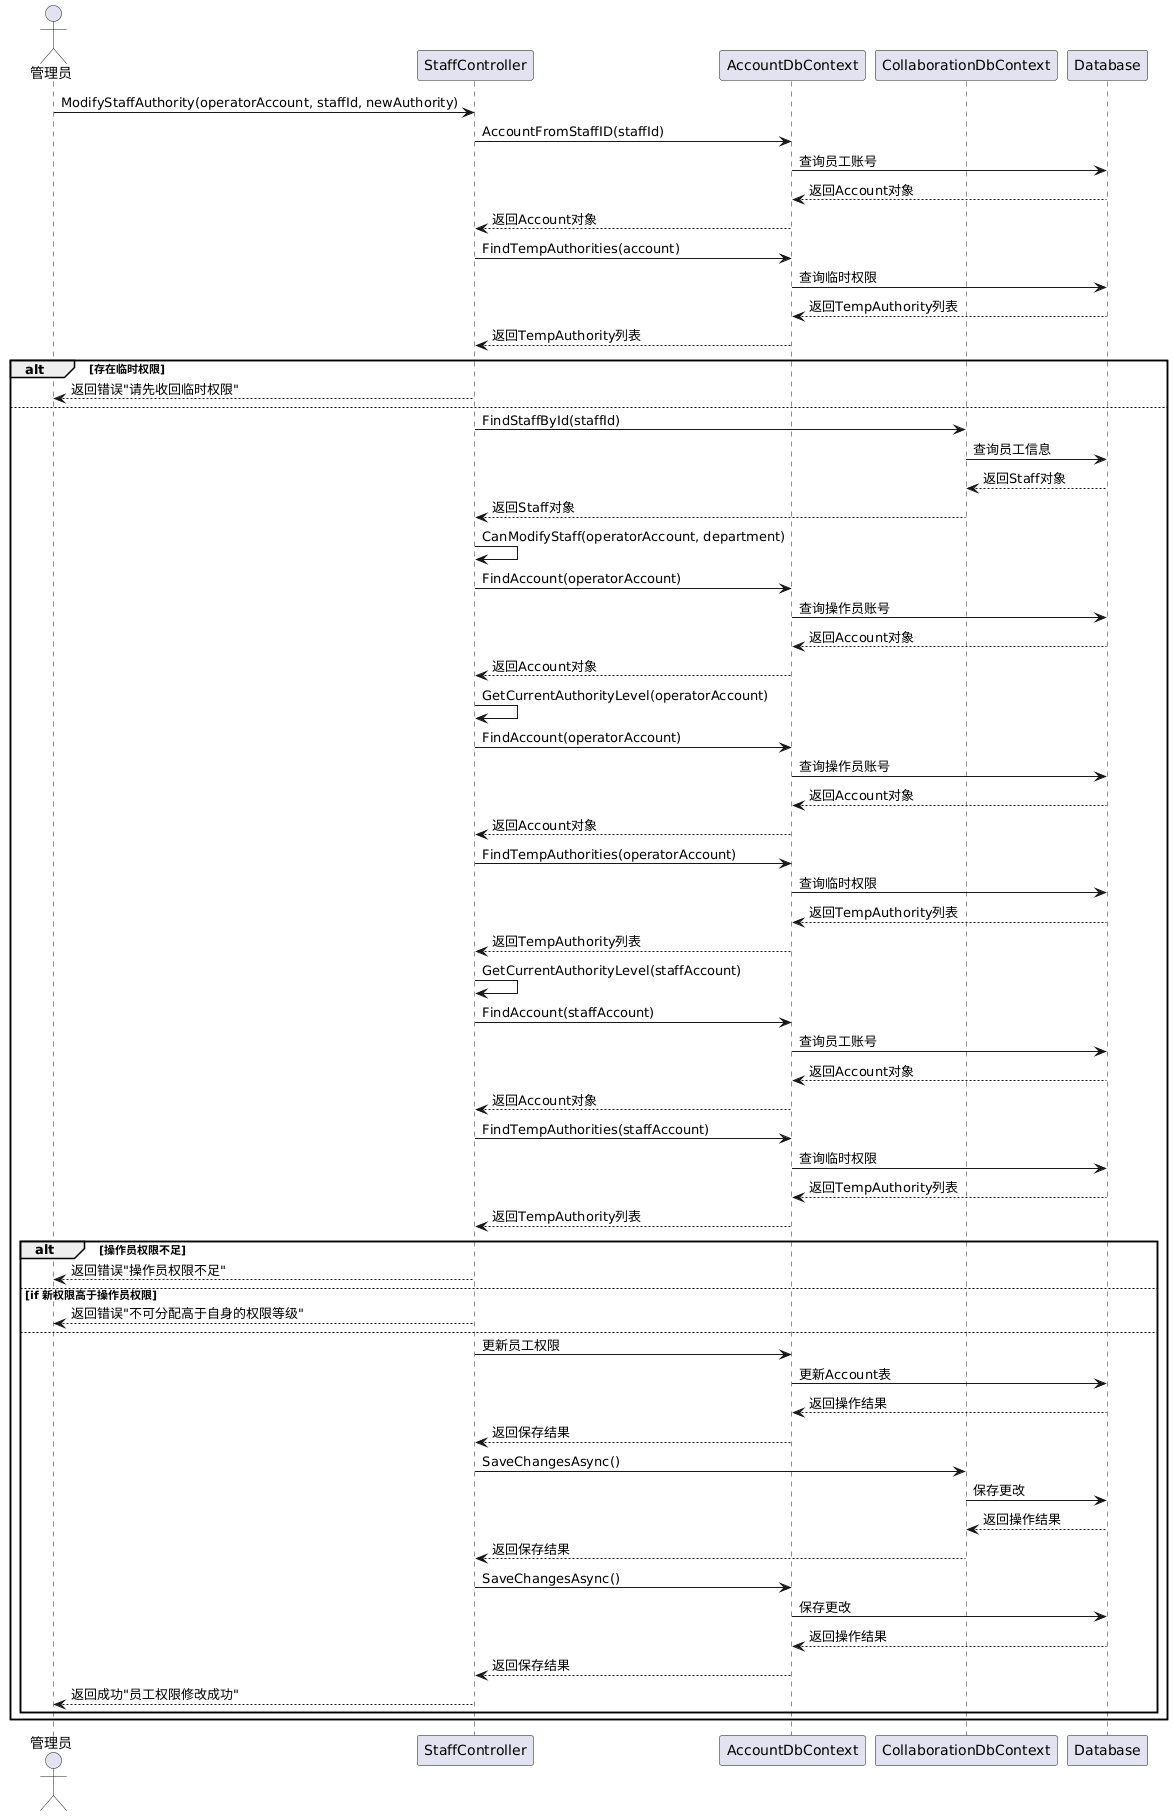
\includegraphics{media/media/image16.png}

促销活动管理活动图:
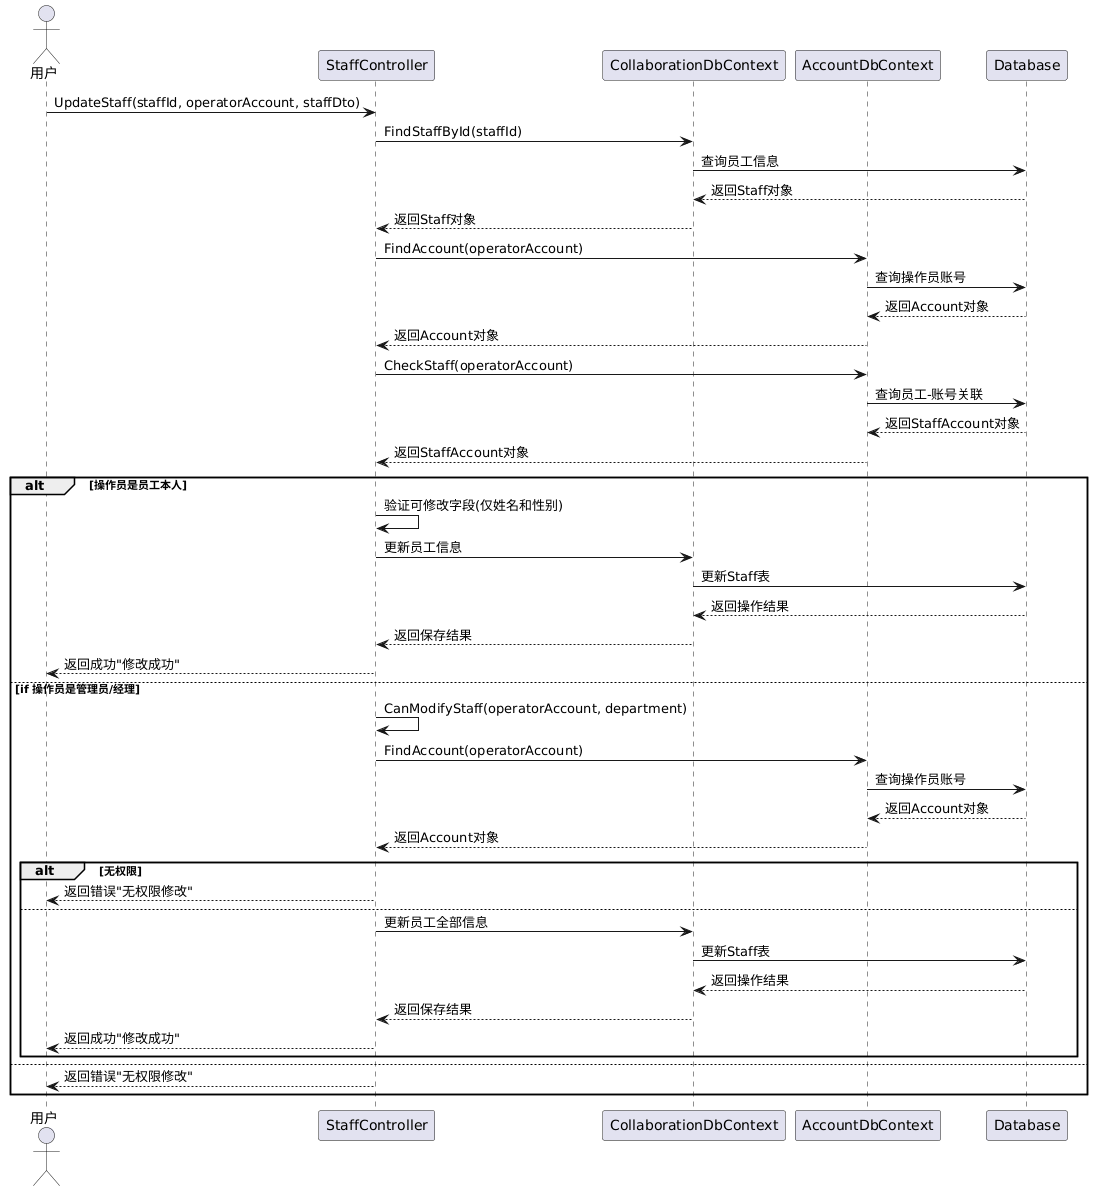
\includegraphics{media/media/image17.png}

促销活动统计报表生成活动图:
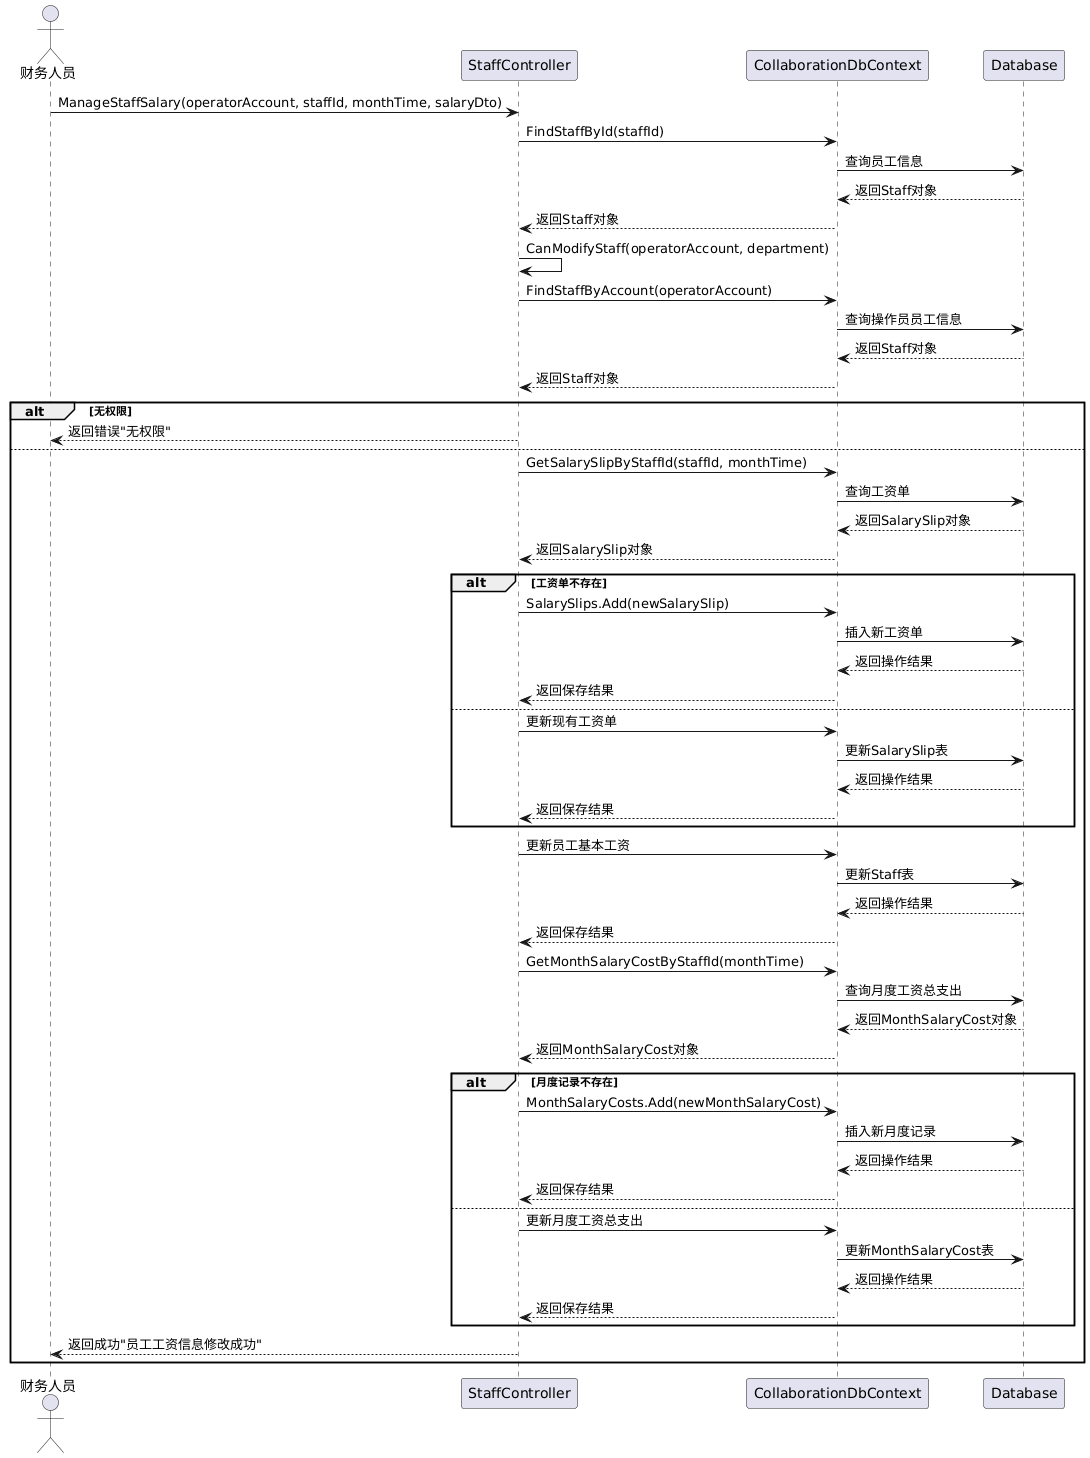
\includegraphics{media/media/image18.png}


\hypertarget{ux6d3bux52a8ux7528ux4f8bux5b9eux73b0}{%
\subsubsection{活动用例实现}\label{ux6d3bux52a8ux7528ux4f8bux5b9eux73b0}}

\subsubsection{场地活动}

1. 主要类及其关系:

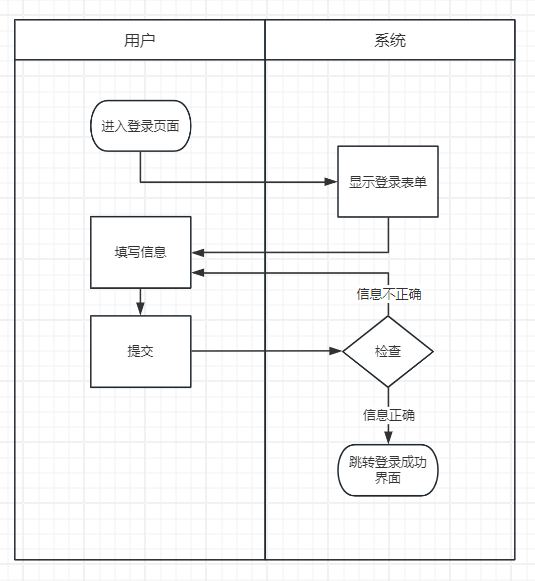
\includegraphics[width=6.2in,height=4.5in]{media/media/image1.png} % Placeholder for Venue Event Class Diagram
\textit{注意:此为类图占位符,需手动替换为实际的UML图。图中应包含VenueEventController、VenueEvent、VenueEventDetail、EventArea、Collaboration等核心类及其关系。}

2. 方法设计与实现:

场地活动预约 (对应需求 2.5.1):
\begin{verbatim}
public class VenueEventReservationDto
{
    [Required] public int CollaborationId { get; set; }
    [Required] public int AreaId { get; set; }
    [Required] public DateTime RentStartTime { get; set; }
    [Required] public DateTime RentEndTime { get; set; }
    public string? RentPurpose { get; set; }
    [Required] public string CollaborationName { get; set; }
    [Required] public string StaffPosition { get; set; }
    [Required] public string EventName { get; set; }
    public int? ExpectedHeadcount { get; set; }
    public double? ExpectedFee { get; set; }
    public int? Capacity { get; set; }
    public int? Expense { get; set; }
}

[HttpPost("reservations")]
public async Task<IActionResult> CreateReservation([FromBody] VenueEventReservationDto dto)
{
    // 验证时间有效性
    if (dto.RentEndTime <= dto.RentStartTime)
    {
        return BadRequest(new { message = "结束时间需晚于起始时间" });
    }

    // 验证活动区域ID是否有效且未被占用
    var eventArea = await _context.EventAreas.FindAsync(dto.AreaId);
    if (eventArea == null)
    {
        return BadRequest(new { message = "活动区域ID无效" });
    }

    // 检查时间段内是否已被占用
    var conflictingReservation = await _context.VenueEventDetails
        .Where(ved => ved.AREA_ID == dto.AreaId &&
                     ved.STATUS != "已取消" &&
                     ((ved.RENT_START <= dto.RentStartTime && ved.RENT_END > dto.RentStartTime) ||
                      (ved.RENT_START < dto.RentEndTime && ved.RENT_END >= dto.RentEndTime) ||
                      (ved.RENT_START >= dto.RentStartTime && ved.RENT_END <= dto.RentEndTime)))
        .FirstOrDefaultAsync();

    if (conflictingReservation != null)
    {
        return BadRequest(new { message = "该区域在指定时间内已被占用" });
    }

    // 验证合作方是否存在
    var collaboration = await _context.Collaborations.FindAsync(dto.CollaborationId);
    if (collaboration == null)
    {
        return BadRequest(new { message = "合作方信息不存在" });
    }

    using var transaction = await _context.Database.BeginTransactionAsync();
    try
    {
        // 创建场地活动记录
        var venueEvent = new VenueEvent
        {
            EVENT_NAME = dto.EventName,
            EVENT_START = dto.RentStartTime,
            EVENT_END = dto.RentEndTime,
            HEADCOUNT = dto.ExpectedHeadcount,
            FEE = dto.ExpectedFee ?? 0,
            CAPACITY = dto.Capacity ?? eventArea.CAPACITY ?? 0,
            EXPENSE = dto.Expense ?? 0
        };

        _context.VenueEvents.Add(venueEvent);
        await _context.SaveChangesAsync();

        // 创建场地活动详情记录
        var venueEventDetail = new VenueEventDetail
        {
            EVENT_ID = venueEvent.EVENT_ID,
            AREA_ID = dto.AreaId,
            COLLABORATION_ID = dto.CollaborationId,
            RENT_START = dto.RentStartTime,
            RENT_END = dto.RentEndTime,
            STATUS = "待审批",
            FUNDING = 0 // 初始资金为0,后续可以更新
        };

        _context.VenueEventDetails.Add(venueEventDetail);
        await _context.SaveChangesAsync();

        await transaction.CommitAsync();

        return Ok(new 
        { 
            message = "场地预约申请提交成功,等待审批",
            eventId = venueEvent.EVENT_ID
        });
    }
    catch (Exception ex)
    {
        await transaction.RollbackAsync();
        _logger.LogError(ex, "创建场地预约失败");
        return StatusCode(500, new { message = "创建场地预约失败" });
    }
}
\end{verbatim}
该方法用于处理场地活动的预约申请。首先,通过 \texttt{VenueEventReservationDto} 接收前端传递的预约信息,包括合作方ID、区域ID、起止时间等。代码逻辑上进行了严格的校验:1. 验证结束时间是否晚于起始时间。2. 确认活动区域ID的有效性。3. 查询数据库,检查申请的时间段内场地是否已被占用,避免资源冲突。所有校验通过后,在一个数据库事务中,同时向 \texttt{VenueEvents} 和 \texttt{VenueEventDetails} 表中插入新的活动记录,初始状态为“待审批”,确保数据的一致性。

场地活动管理 (对应需求 2.5.2):
\begin{verbatim}
public class VenueEventUpdateDto
{
    public string? EventName { get; set; }
    public int? Headcount { get; set; }
    public string? Description { get; set; }
    public string? Status { get; set; } // 筹备中/进行中/已结束/已取消
    public List<string>? ParticipantAccounts { get; set; }
}

[HttpPut("events/{eventId}")]
public async Task<IActionResult> UpdateVenueEvent(int eventId, [FromBody] VenueEventUpdateDto dto)
{
    var venueEvent = await _context.VenueEvents.FindAsync(eventId);
    if (venueEvent == null)
    {
        return NotFound(new { message = "找不到对应的活动记录" });
    }

    var venueEventDetail = await _context.VenueEventDetails
        .FirstOrDefaultAsync(ved => ved.EVENT_ID == eventId);

    if (venueEventDetail == null)
    {
        return NotFound(new { message = "找不到对应的活动详情记录" });
    }

    // 检查活动是否已结束
    if (venueEventDetail.STATUS == "已结束")
    {
        return BadRequest(new { message = "活动已结束,不可修改或取消" });
    }

    try
    {
        // 更新活动信息
        if (!string.IsNullOrEmpty(dto.EventName))
            venueEvent.EVENT_NAME = dto.EventName;

        if (dto.Headcount.HasValue)
            venueEvent.HEADCOUNT = dto.Headcount.Value;

        if (!string.IsNullOrEmpty(dto.Status))
            venueEventDetail.STATUS = dto.Status;

        // 处理批量导入参与人员
        if (dto.ParticipantAccounts != null && dto.ParticipantAccounts.Any())
        {
            // 删除现有临时权限
            var existingTempAuthorities = await _context.TempAuthorities
                .Where(ta => ta.EVENT_ID == eventId)
                .ToListAsync();
            _context.TempAuthorities.RemoveRange(existingTempAuthorities);

            // 添加新的临时权限
            foreach (var account in dto.ParticipantAccounts)
            {
                var tempAuthority = new TempAuthority
                {
                    ACCOUNT = account,
                    EVENT_ID = eventId,
                    TEMP_AUTHORITY = 3 // 普通员工权限
                };
                _context.TempAuthorities.Add(tempAuthority);
            }
        }

        await _context.SaveChangesAsync();

        return Ok(new { message = "活动信息更新成功" });
    }
    catch (Exception ex)
    {
        _logger.LogError(ex, $"更新活动 {eventId} 失败");
        return StatusCode(500, new { message = "更新活动失败" });
    }
}
\end{verbatim}
此方法允许授权用户修改已存在的场地活动信息。它首先会校验活动是否存在且状态不是“已结束”。\texttt{VenueEventUpdateDto} 允许部分更新,只有传入的字段才会被修改。特别地,该方法支持通过 \texttt{ParticipantAccounts} 列表批量更新参与活动的员工,系统会先清除该活动所有旧的临时权限,再根据新列表授予新的临时权限,实现了对活动参与人员的动态管理。

场地活动结算收费 (对应需求 2.5.3):
\begin{verbatim}
[HttpPost("events/{eventId}/settlement")]
public async Task<IActionResult> CreateSettlement(int eventId, [FromBody] VenueEventSettlementDto dto)
{
    var venueEventDetail = await _context.VenueEventDetails
        .Include(ved => ved.venueEventNavigation)
        .Include(ved => ved.eventAreaNavigation)
        .FirstOrDefaultAsync(ved => ved.EVENT_ID == eventId);

    if (venueEventDetail == null)
    {
        return NotFound(new { message = "找不到对应的活动记录" });
    }

    if (venueEventDetail.STATUS != "已结束")
    {
        return BadRequest(new { message = "只有已结束的活动才能进行结算" });
    }

    try
    {
        // 计算租用时长(小时)
        var rentHours = (venueEventDetail.RENT_END - venueEventDetail.RENT_START).TotalHours;
        
        // 计算总费用
        var totalFee = dto.VenueFee + (dto.AdditionalServiceFee ?? 0);

        // 创建结算信息用于返回
        var settlementInfo = new
        {
            EventId = eventId,
            EventName = venueEventDetail.venueEventNavigation.EVENT_NAME,
            AreaId = venueEventDetail.AREA_ID,
            RentStart = venueEventDetail.RENT_START,
            RentEnd = venueEventDetail.RENT_END,
            RentHours = Math.Round(rentHours, 2),
            VenueFee = dto.VenueFee,
            AdditionalServiceFee = dto.AdditionalServiceFee ?? 0,
            TotalFee = totalFee,
            PaymentMethod = dto.PaymentMethod,
            InvoiceInfo = dto.InvoiceInfo,
            SettlementTime = DateTime.Now
        };

        // 更新活动状态为已结算,并将总费用存储到FUNDING字段
        venueEventDetail.STATUS = "已结算";
        venueEventDetail.FUNDING = totalFee;  // 新增:将总费用存储到FUNDING字段
        await _context.SaveChangesAsync();

        return Ok(new 
        { 
            message = "结算单生成成功",
            settlement = settlementInfo
        });
    }
    catch (Exception ex)
    {
        _logger.LogError(ex, $"创建结算单 {eventId} 失败");
        return StatusCode(500, new { message = "创建结算单失败" });
    }
}
\end{verbatim}
当活动状态更新为“已结束”后,可通过此方法进行结算。方法会校验活动状态,然后根据 \texttt{VenueEventSettlementDto} 中提供的费用信息,计算出总费用。计算完成后,将活动状态更新为“已结算”,并将总费用记录到 \texttt{FUNDING} 字段,最后返回详细的结算单信息给前端。

场地活动统计报表生成 (对应需求 2.5.4):
\begin{verbatim}
[HttpGet("reports")]
public async Task<IActionResult> GenerateReport([FromQuery] VenueEventReportRequestDto dto)
{
    if (dto.EndDate <= dto.StartDate)
    {
        return BadRequest(new { message = "结束时间需晚于起始时间" });
    }

    try
    {
        var events = await _context.VenueEventDetails
            .Include(ved => ved.venueEventNavigation)
            .Include(ved => ved.eventAreaNavigation)
            .Where(ved => ved.RENT_START >= dto.StartDate && ved.RENT_END <= dto.EndDate)
            .ToListAsync();

        if (!events.Any())
        {
            return Ok(new { message = "该时间段内无场地活动记录" });
        }

        // 计算统计数据
        var totalEvents = events.Count;
        var totalRentHours = events.Sum(e => (e.RENT_END - e.RENT_START).TotalHours);
        var totalRevenue = events.Sum(e => (e.eventAreaNavigation?.AREA_FEE ?? 0) * 
                                           (e.RENT_END - e.RENT_START).TotalHours);

        // 计算平均上座率
        var eventsWithCapacity = events.Where(e => e.venueEventNavigation.CAPACITY > 0).ToList();
        var averageOccupancy = eventsWithCapacity.Any() ? 
            eventsWithCapacity.Average(e => (double)(e.venueEventNavigation.HEADCOUNT ?? 0) / e.venueEventNavigation.CAPACITY * 100) : 0;

        // 热门场地排行
        var popularVenues = events
            .GroupBy(e => e.AREA_ID)
            .Select(g => new PopularVenueDto
            {
                AreaId = g.Key,
                EventCount = g.Count(),
                TotalRevenue = g.Sum(e => (e.eventAreaNavigation?.AREA_FEE ?? 0) * 
                                          (e.RENT_END - e.RENT_START).TotalHours)
            })
            .OrderByDescending(p => p.EventCount)
            .Take(10)
            .ToList();

        // 活动详情
        var eventDetails = events.Select(e => new VenueEventSummaryDto
        {
            EventId = e.EVENT_ID,
            EventName = e.venueEventNavigation.EVENT_NAME,
            AreaId = e.AREA_ID,
            RentStart = e.RENT_START,
            RentEnd = e.RENT_END,
            RentHours = Math.Round((e.RENT_END - e.RENT_START).TotalHours, 2),
            VenueFee = (e.eventAreaNavigation?.AREA_FEE ?? 0) * (e.RENT_END - e.RENT_START).TotalHours,
            ActualHeadcount = e.venueEventNavigation.HEADCOUNT,
            Status = e.STATUS
        }).ToList();

        var report = new VenueEventReportDto
        {
            TotalEvents = totalEvents,
            TotalRentHours = Math.Round(totalRentHours, 2),
            TotalRevenue = Math.Round(totalRevenue, 2),
            AverageOccupancy = Math.Round(averageOccupancy, 2),
            PopularVenues = popularVenues,
            EventDetails = eventDetails
        };

        return Ok(report);
    }
    catch (Exception ex)
    {
        _logger.LogError(ex, "生成统计报表失败");
        return StatusCode(500, new { message = "生成统计报表失败" });
    }
}
\end{verbatim}
该方法用于生成场地活动的统计报表。它接收一个包含起止日期的 \texttt{VenueEventReportRequestDto} 对象,查询在此时间范围内的所有活动。然后,它会进行一系列的聚合计算,包括活动总数、总租用时长、总收入、平均上座率(基于活动容量和实际参与人数),并根据活动次数对场地进行排名,最终生成一份全面的统计报告。

\subsubsection{促销活动}

1. 主要类及其关系:

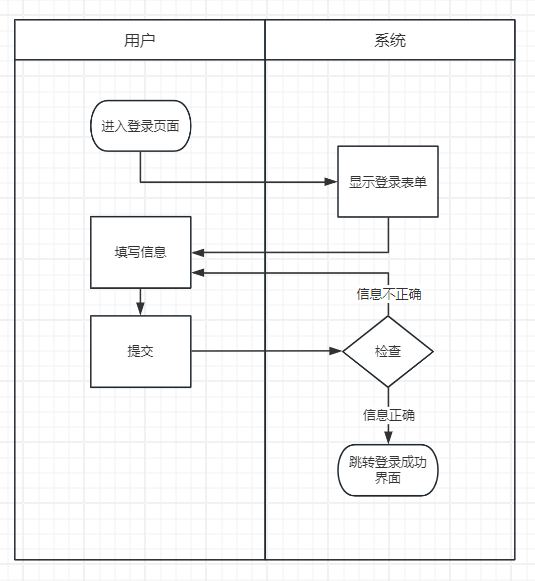
\includegraphics[width=6.2in,height=4.5in]{media/media/image1.png} % Placeholder for Sale Event Class Diagram
\textit{注意:此为类图占位符,需手动替换为实际的UML图。图中应包含SaleEventController、SaleEventService、SaleEvent、PartStore、Store等核心类及其关系。}

2. 方法设计与实现:

新增促销活动 (对应需求 2.5.5):
\begin{verbatim}
public class SaleEventDto
{
    public string EventName { get; set; }
    public double Cost { get; set; }
    public DateTime EventStart { get; set; }
    public DateTime EventEnd { get; set; }
    public string Description { get; set; }
}

public async Task<SaleEvent> CreateSaleEventAsync(SaleEventDto dto)
{
    if (dto.EventStart > dto.EventEnd)
        throw new ArgumentException("结束时间必须晚于开始时间");
    int? maxId = await _context.SaleEvents.MaxAsync(e => (int?)e.EVENT_ID);
    int newId = (maxId ?? 0) + 1;
    var saleEvent = new SaleEvent
    {
        EVENT_ID = newId,
        EVENT_NAME = dto.EventName,
        Cost = dto.Cost,
        EVENT_START = dto.EventStart,
        EVENT_END = dto.EventEnd,
        Description = dto.Description,
    };
    _context.SaleEvents.Add(saleEvent);
    await _context.SaveChangesAsync();
    return saleEvent;
}
\end{verbatim}
此方法在 \texttt{SaleEventService} 中实现,用于创建新的促销活动。它首先通过 \texttt{SaleEventDto} 接收活动信息,并校验时间的有效性。为了确保ID的唯一性,它会查询当前最大的 \texttt{EVENT\_ID} 并在此基础上加一作为新ID。最后,创建一个新的 \texttt{SaleEvent} 实例并将其存入数据库。

促销活动管理 (对应需求 2.5.6):
\begin{verbatim}
public async Task<SaleEvent> UpdateSaleEventAsync(int id, SaleEventDto dto)
{
    var saleEvent = await _context.SaleEvents.FindAsync(id);
    if (saleEvent == null)
        throw new KeyNotFoundException("促销活动不存在");
    
    if (!string.IsNullOrEmpty(dto.EventName)) saleEvent.EVENT_NAME = dto.EventName;
    if (dto.Cost > 0) saleEvent.Cost = dto.Cost;
    if (!string.IsNullOrEmpty(dto.Description)) saleEvent.Description = dto.Description;
    if (dto.EventStart != default) saleEvent.EVENT_START = dto.EventStart;
    if (dto.EventEnd != default) saleEvent.EVENT_END = dto.EventEnd;

    await _context.SaveChangesAsync();
    return saleEvent;
}
\end{verbatim}
在 \texttt{SaleEventService} 中,此方法用于更新一个已存在的促销活动。它首先根据ID查找活动,如果未找到则抛出异常。然后,它会检查 \texttt{SaleEventDto} 中的每个字段,只有当字段有新值时才进行更新,这允许了对活动的增量式修改。

促销活动统计报表生成 (对应需求 2.5.7):
\begin{verbatim}
public async Task<SaleEventReport> GenerateSaleEventReportAsync(int eventId)
{
    var saleEvent = await _context.SaleEvents.FindAsync(eventId);
    if (saleEvent == null)
        throw new KeyNotFoundException("促销活动不存在");
    
    var reportData = await FetchSalesDataFromExternalSystem(saleEvent);

    return new SaleEventReport
    {
        EventId = saleEvent.EVENT_ID,
        EventName = saleEvent.EVENT_NAME,
        SalesIncrement = reportData.SalesIncrement,
        Cost = saleEvent.Cost,
        ROI = CalculateROI(reportData.SalesIncrement, saleEvent.Cost),
        CouponRedemptionRate = reportData.CouponRedemptionRate
    };
}
\end{verbatim}
此方法同样在 \texttt{SaleEventService} 中实现,用于生成单个促销活动的效果报告。它首先获取活动的基本信息,然后通过一个模拟的 \texttt{FetchSalesDataFromExternalSystem} 方法来获取与活动相关的销售数据(如销售增量、优惠券核销率)。最后,它会基于成本和销售增量计算投资回报率(ROI),并将所有统计数据封装在 \texttt{SaleEventReport} 对象中返回。

\hypertarget{ux5546ux6237ux7528ux4f8b}{%
\subsection{商户用例}\label{ux5546ux6237ux7528ux4f8b}}

\hypertarget{ux5546ux6237ux7528ux4f8bux8bbeux8ba1}{%
\subsubsection{商户用例设计}\label{ux5546ux6237ux7528ux4f8bux8bbeux8ba1}}

表格 2-9 商户功能的动作序列
\begin{longtable}[]{@{}ll@{}}
\toprule
动作序列 & 描述\tabularnewline
\midrule
\endhead
新增商户 & 管理员录入新商户信息,关联租用的店面,并创建商户账号。\tabularnewline
商户信息管理 & 管理员可修改商户核心信息,商户可修改联系方式等非核心信息。\tabularnewline
新增店面 & 物业管理人员添加新的店面区域,录入面积、租金等信息。\tabularnewline
店面状态管理 & 商户提交状态变更申请(如退租、维修),物业审批后系统更新。\tabularnewline
商户信息统计报表 & 系统按租户类型、店面区域等维度生成商户统计报表。\tabularnewline
商户租金收取 & 系统计算商户应缴租金,商户通过账号缴纳,财务人员确认收款。\tabularnewline
商户租金统计报表 & 系统按时间、区域等维度统计租金收入。\tabularnewline
\bottomrule
\end{longtable}

\textit{注意:由于空间限制,此处的活动图均使用占位符,实际文档中需替换为对应的图表。}

新增商户活动图:
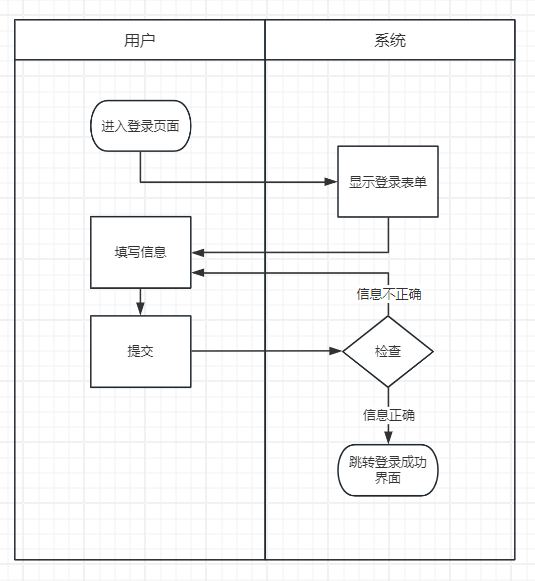
\includegraphics{media/media/image1.png}

商户信息管理活动图:
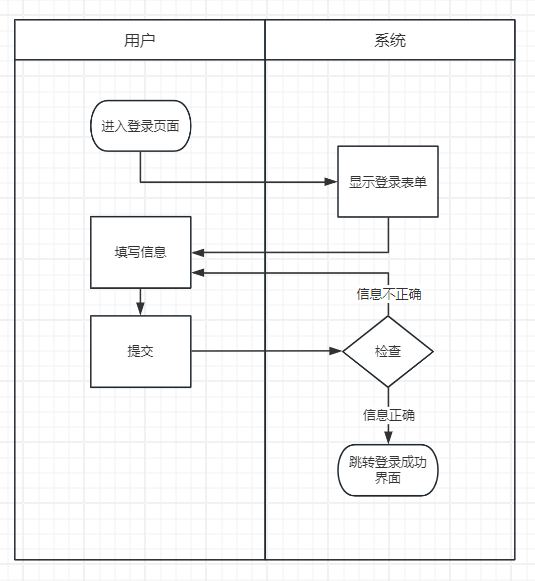
\includegraphics{media/media/image1.png}

新增店面活动图:
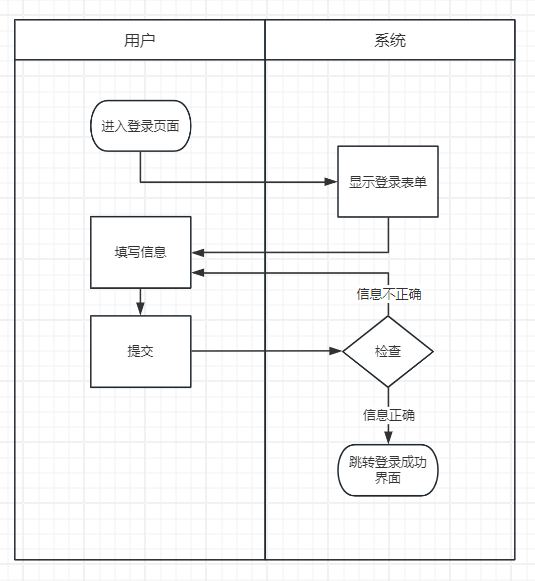
\includegraphics{media/media/image1.png}

店面状态管理活动图:
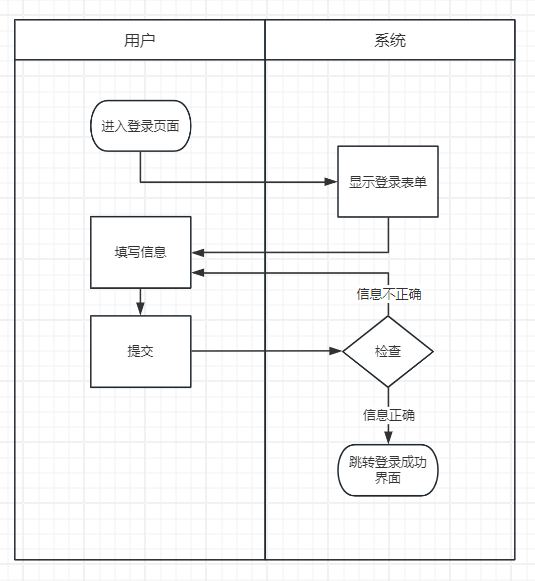
\includegraphics{media/media/image1.png}

商户信息统计报表活动图:
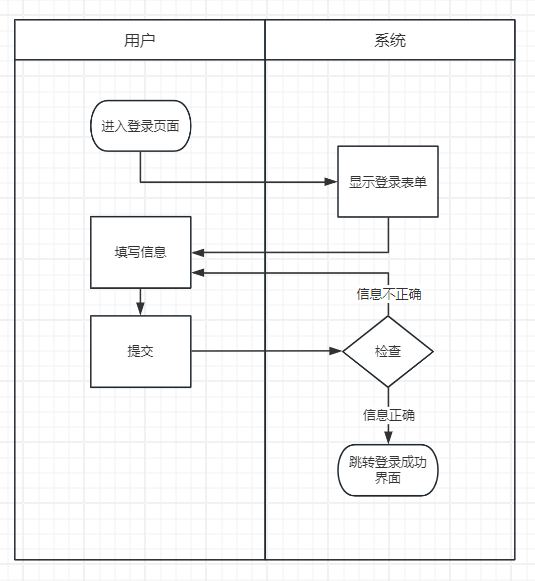
\includegraphics{media/media/image1.png}

商户租金收取活动图:
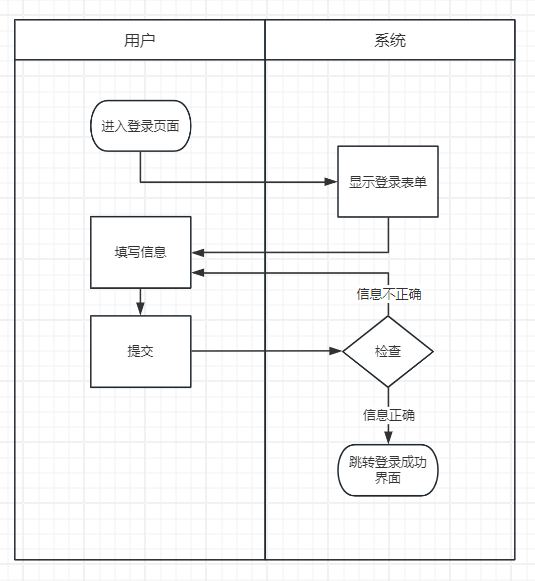
\includegraphics{media/media/image1.png}

商户租金统计报表活动图:
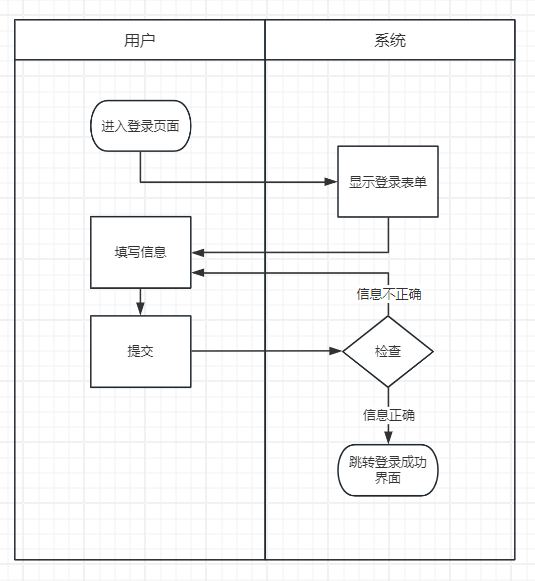
\includegraphics{media/media/image1.png}

\hypertarget{ux5546ux6237ux7528ux4f8bux5b9eux73b0}{%
\subsubsection{商户用例实现}\label{ux5546ux6237ux7528ux4f8bux5b9eux73b0}}

1. 主要类及其关系:

\includegraphics[width=6.2in,height=4.5in]{media/media/image1.png} % Placeholder for Merchant Module Class Diagram
\textit{注意:此为类图占位符,需手动替换为实际的UML图。图中应包含StoreController、Store、RetailArea、RentStore、StoreAccount等核心类及其关系。}

2. 方法设计与实现:

\textbf{新增店面 (对应需求 2.7.3):}
\begin{verbatim}
public class CreateRetailAreaDto
{
    [Required] public int AreaId { get; set; }
    [Required] public int AreaSize { get; set; }
    [Required] public double BaseRent { get; set; }
    [Required] public string OperatorAccount { get; set; }
}

[HttpPost("CreateRetailArea")]
public async Task<IActionResult> CreateRetailArea([FromBody] CreateRetailAreaDto dto)
{
    _logger.LogInformation("开始新增店面区域:{AreaId}", dto.AreaId);

    // 检查模型验证
    if (!ModelState.IsValid)
    {
        var errors = ModelState.Values
            .SelectMany(v => v.Errors)
            .Select(e => e.ErrorMessage)
            .ToList();
        _logger.LogWarning("新增店面模型验证失败:{Errors}", string.Join(", ", errors));
        return BadRequest(new { error = "输入数据验证失败", details = errors });
    }

    try
    {
        // 1. 验证操作员权限(管理员权限)
        if (!string.IsNullOrEmpty(dto.OperatorAccount))
        {
            var hasPermission = await _accountContext.CheckAuthority(dto.OperatorAccount, 1);
            if (!hasPermission)
            {
                _logger.LogWarning("操作员 {OperatorAccount} 权限不足", dto.OperatorAccount);
                return BadRequest(new { error = "操作员权限不足,需要管理员权限" });
            }
        }

        // 2. 校验区域ID唯一性
        var existingArea = await _storeContext.AREA.FirstOrDefaultAsync(a => a.AREA_ID == dto.AreaId);
        if (existingArea != null)
        {
            _logger.LogWarning("区域ID {AreaId} 已存在", dto.AreaId);
            return BadRequest(new { error = "该区域ID已存在,请重新设置" });
        }

        // 4. 创建零售区域记录
        var retailArea = new RetailArea
        {
            AREA_ID = dto.AreaId,
            ISEMPTY = 1, // 新建区域默认为空置状态
            AREA_SIZE = dto.AreaSize,
            CATEGORY = "RETAIL",
            RENT_STATUS = "空置", // 新建店面默认为空置状态
            BASE_RENT = dto.BaseRent
        };

        _storeContext.RETAIL_AREA.Add(retailArea);
        await _storeContext.SaveChangesAsync();

        _logger.LogInformation("成功创建店面区域:{AreaId},面积:{AreaSize},租金:{BaseRent}", 
            dto.AreaId, dto.AreaSize, dto.BaseRent);

        // 返回创建成功的信息
        return Ok(new
        {
            message = "店面区域创建成功",
            areaId = dto.AreaId,
            areaSize = dto.AreaSize,
            baseRent = dto.BaseRent,
            rentStatus = "空置",
            isEmpty = 1
        });
    }
    catch (Exception ex)
    {
        _logger.LogError(ex, "创建店面区域时发生错误:{AreaId}", dto.AreaId);
        
        if (ex.InnerException?.Message?.Contains("ORA-00001") == true || 
            ex.InnerException?.Message?.Contains("UNIQUE") == true)
        {
            return BadRequest(new { error = "该区域ID已存在,请重新设置" });
        }
        
        return StatusCode(500, new { 
            error = "服务器内部错误,创建店面区域失败",
            details = ex.Message
        });
    }
}
\end{verbatim}
该方法允许具备管理员权限的操作员添加新的店面区域。它首先通过 `CreateRetailAreaDto` 接收区域ID、面积和基础租金。在执行前,系统会严格校验操作员的权限,并查询数据库确保区域ID的唯一性,防止重复录入。校验通过后,一个新的 `RetailArea` 记录将被创建并保存到数据库,其初始状态自动设置为“空置”,为后续的招商工作做好准备。

\textbf{新增商户 (对应需求 2.7.1):}
\begin{verbatim}
public class CreateMerchantDto
{
    [Required] public string StoreName { get; set; }
    [Required] public string StoreType { get; set; }
    [Required] public string TenantName { get; set; }
    [Required] public string ContactInfo { get; set; }
    [Required] public int AreaId { get; set; }
    [Required] public DateTime RentStart { get; set; }
    [Required] public DateTime RentEnd { get; set; }
    public string? OperatorAccount { get; set; }
}

[HttpPost("CreateMerchant")]
public async Task<IActionResult> CreateMerchant([FromBody] CreateMerchantDto dto)
{
    _logger.LogInformation("开始创建新商户:{StoreName}", dto.StoreName);

    if (!ModelState.IsValid)
    {
        return BadRequest(ModelState);
    }

    try
    {
        if (!string.IsNullOrEmpty(dto.OperatorAccount))
        {
            var hasPermission = await _accountContext.CheckAuthority(dto.OperatorAccount, 1);
            if (!hasPermission)
            {
                return BadRequest(new { error = "操作员权限不足" });
            }
        }

        if (dto.RentEnd <= dto.RentStart || dto.RentStart.Date < DateTime.Today)
        {
            return BadRequest(new { error = "租用时间无效" });
        }

        if (!await _storeContext.IsAreaAvailable(dto.AreaId))
        {
            return BadRequest(new { error = "该店面已租用" });
        }

        if (await _storeContext.TenantExists(dto.TenantName, dto.ContactInfo))
        {
            return BadRequest(new { error = "该租户已在本综合体有店铺" });
        }

        var storeId = await _storeContext.GetNextStoreId();
        var store = new Store { /* ... a ... */ };
        _storeContext.STORE.Add(store);

        var rentStore = new RentStore { STORE_ID = storeId, AREA_ID = dto.AreaId };
        _storeContext.RENT_STORE.Add(rentStore);

        await _storeContext.UpdateAreaStatus(dto.AreaId, false, "已租用");

        var accountName = $"store_{storeId:D6}";
        var initialPassword = "password123"; // Simplified
        var merchantAccount = new Account { /* ... b ... */ };
        _accountContext.ACCOUNT.Add(merchantAccount);

        var storeAccount = new StoreAccount { ACCOUNT = accountName, STORE_ID = storeId };
        _accountContext.STORE_ACCOUNT.Add(storeAccount);

        await _storeContext.SaveChangesAsync();
        await _accountContext.SaveChangesAsync();

        return Ok(new { message = "商户创建成功", storeId, accountName, initialPassword });
    }
    catch (Exception ex)
    {
        _logger.LogError(ex, "创建商户失败");
        return StatusCode(500, "服务器内部错误");
    }
}
\end{verbatim}
此方法用于招商管理,将一个空置的店面分配给新商户。它执行一系列严格的校验,包括操作员权限、租用时间的合理性、店面是否确实处于“空置”状态,以及租户信息是否已存在。所有条件满足后,在一个事务性操作中,系统会:1. 创建新的 \texttt{Store} 记录;2. 在 \texttt{RentStore} 中建立店铺与区域的关联;3. 将对应 \texttt{RetailArea} 的状态更新为“已租用”;4. 自动为商户生成一个格式化的系统账号(如 \texttt{store\_000001})和初始密码,并赋予商户权限。

\textbf{商户信息管理 (对应需求 2.7.2):}
\begin{verbatim}
public class UpdateMerchantInfoDto
{
    [Required] public int StoreId { get; set; }
    public string? ContactInfo { get; set; } // 商户可改
    public string? StoreType { get; set; } // 管理员可改
    public DateTime? RentStart { get; set; } // 管理员可改
    public DateTime? RentEnd { get; set; } // 管理员可改
    public string? StoreStatus { get; set; } // 管理员可改
    [Required] public string OperatorAccount { get; set; }
}

[HttpPut("UpdateMerchantInfo")]
public async Task<IActionResult> UpdateMerchantInfo([FromBody] UpdateMerchantInfoDto dto)
{
    _logger.LogInformation("开始更新商户信息:{StoreId}", dto.StoreId);

    try
    {
        var operator_account = await _accountContext.FindAccount(dto.OperatorAccount);
        if (operator_account == null) return BadRequest("操作员账号不存在");

        bool isAdmin = operator_account.AUTHORITY <= 2;
        bool isMerchant = !isAdmin && await _accountContext.STORE_ACCOUNT.AnyAsync(sa => sa.ACCOUNT == dto.OperatorAccount && sa.STORE_ID == dto.StoreId);

        if (!isAdmin && !isMerchant) return BadRequest("无权限修改");

        var store = await _storeContext.GetStoreById(dto.StoreId);
        if (store == null) return NotFound("店铺不存在");

        if (store.STORE_STATUS != "正常营业" && store.STORE_STATUS != "歇业中")
        {
            return BadRequest("当前商户状态不允许修改信息");
        }

        bool hasChanges = false;
        if (!string.IsNullOrEmpty(dto.ContactInfo)) { store.CONTACT_INFO = dto.ContactInfo; hasChanges = true; }

        if (isAdmin)
        {
            if (!string.IsNullOrEmpty(dto.StoreType)) { store.STORE_TYPE = dto.StoreType; hasChanges = true; }
            // ... other admin-only fields
        }
        else if (dto.StoreType != null || dto.StoreStatus != null)
        {
            return BadRequest("无权限修改核心信息");
        }

        if (!hasChanges) return BadRequest("没有需要更新的信息");

        await _storeContext.SaveChangesAsync();
        return Ok(new { message = "商户信息更新成功" });
    }
    catch (Exception ex)
    {
        _logger.LogError(ex, "更新商户信息失败");
        return StatusCode(500, "服务器内部错误");
    }
}
\end{verbatim}
该方法实现了分权管理商户信息。系统首先会判断操作员的身份:如果是管理员(权限等级≤2),则可以修改所有核心信息,如租户类型、租期和店铺状态;如果操作员是与该店铺关联的商户账号,则只能修改联系方式等非核心信息。这种设计确保了数据的安全性和权责的清晰分离。

\textbf{店面状态管理 (对应需求 2.7.4):}
\begin{verbatim}
public class StoreStatusChangeRequestDto
{
    [Required] public int StoreId { get; set; }
    [Required] public string ChangeType { get; set; } // 退租/维修等
    [Required] public string Reason { get; set; }
    [Required] public string TargetStatus { get; set; }
    [Required] public string ApplicantAccount { get; set; }
}

[HttpPost("StatusChangeRequest")]
public async Task<IActionResult> SubmitStatusChangeRequest([FromBody] StoreStatusChangeRequestDto dto)
{
    try
    {
        var store = await _storeContext.GetStoreById(dto.StoreId);
        if (store == null) return BadRequest("店面不存在");

        // ... (validation logic)

        var applicationNo = "SA" + DateTime.Now.ToString("yyyyMMddHHmmss");
        _logger.LogInformation("状态变更申请详情:{ApplicationNo}", applicationNo);

        return Ok(new { message = "状态变更申请提交成功", applicationNo });
    }
    catch (Exception ex)
    {
        _logger.LogError(ex, "提交状态变更申请失败");
        return StatusCode(500, "服务器内部错误");
    }
}

[HttpPost("ApproveStatusChange")]
public async Task<IActionResult> ApproveStatusChange([FromBody] StoreStatusApprovalDto dto)
{
    try
    {
        var hasPermission = await _accountContext.CheckAuthority(dto.ApproverAccount, 2);
        if (!hasPermission) return BadRequest("权限不足");

        var store = await _storeContext.GetStoreById(dto.StoreId);
        if (store == null) return BadRequest("店面不存在");

        if (dto.ApprovalAction == "通过")
        {
            store.STORE_STATUS = dto.TargetStatus;
            await _storeContext.SaveChangesAsync();
            return Ok(new { message = "审批通过,店面状态已更新" });
        }
        else
        {
            return Ok(new { message = "审批驳回" });
        }
    }
    catch (Exception ex)
    {
        _logger.LogError(ex, "处理状态变更审批失败");
        return StatusCode(500, "服务器内部错误");
    }
}
\end{verbatim}
这是一个两步式的工作流。首先,商户或管理员通过 `SubmitStatusChangeRequest` 接口提交状态变更申请,系统会根据当前店面状态验证申请的合理性(如“正常营业”的店面才能申请“退租”),然后生成一个待审批的申请记录。接着,具备权限的物业管理员通过 `ApproveStatusChange` 接口对申请进行“通过”或“驳回”操作。如果通过,系统将正式更新店面的状态。

\textbf{商户信息统计报表 (对应需求 2.7.5):}
\begin{verbatim}
[HttpGet("MerchantStatisticsReport")]
public async Task<IActionResult> GetMerchantStatisticsReport([FromQuery] string operatorAccount, [FromQuery] string dimension = "all")
{
    try
    {
        var hasPermission = await _accountContext.CheckAuthority(operatorAccount, 2);
        if (!hasPermission)
        {
            return BadRequest(new { error = "权限不足" });
        }

        object reportData;
        switch (dimension.ToLower())
        {
            case "type":
                reportData = await _storeContext.GetStoreStatisticsByType();
                break;
            case "area":
                reportData = await _storeContext.GetStoreStatisticsByArea();
                break;
            case "status":
                reportData = await _storeContext.GetStoreStatisticsByStatus();
                break;
            default:
                reportData = new {
                    byType = await _storeContext.GetStoreStatisticsByType(),
                    byArea = await _storeContext.GetStoreStatisticsByArea(),
                    byStatus = await _storeContext.GetStoreStatisticsByStatus()
                };
                break;
        }

        return Ok(new { reportTitle = "商户信息统计报表", data = reportData });
    }
    catch (Exception ex)
    {
        _logger.LogError(ex, "生成商户统计报表失败");
        return StatusCode(500, "生成报表失败");
    }
}
\end{verbatim}
此方法为管理层提供决策支持。它要求操作员具备管理员权限,并允许通过 `dimension` 参数指定不同的统计维度。例如,当 `dimension` 为 `type` 时,系统会按租户类型(如“餐饮”、“零售”)进行分组统计;当为 `area` 时,则按物理区域进行分析。这使得管理者可以从不同视角审视商户的构成和分布情况。

\textbf{商户租金收取 (对应需求 2.7.6):}
\begin{verbatim}
[HttpPost("GenerateMonthlyRentBills")]
public async Task<IActionResult> GenerateMonthlyRentBills([FromBody] string billPeriod)
{
    try
    {
        if (string.IsNullOrEmpty(billPeriod) || billPeriod.Length != 6)
        {
            return BadRequest("账期格式错误");
        }
        var bills = await _storeContext.GenerateMonthlyRentBills(billPeriod);
        return Ok(new { message = $"成功生成{bills.Count}张租金单", generatedBills = bills.Count });
    }
    catch (Exception ex)
    {
        _logger.LogError(ex, "生成月度租金单失败");
        return StatusCode(500, "生成租金单失败");
    }
}

[HttpPost("PayRent")]
public async Task<IActionResult> PayRent([FromBody] PayRentRequest request)
{
    try
    {
        var success = await _storeContext.ProcessRentPayment(request);
        if (!success)
        {
            return BadRequest("支付失败");
        }
        return Ok(new { message = "租金支付成功" });
    }
    catch (Exception ex)
    {
        _logger.LogError(ex, "处理租金支付失败");
        return StatusCode(500, "支付处理失败");
    }
}
\end{verbatim}
租金管理是商户模块的核心。`GenerateMonthlyRentBills` 通常由系统定时任务或管理员手动触发,为所有在租状态的商户生成指定月份的租金账单。商户登录后,可以通过 `GetMyRentBills` 查询到自己的账单,然后调用 `PayRent` 接口完成支付。系统会记录支付信息并更新账单状态。

\textbf{商户租金统计报表 (对应需求 2.7.7):}
\begin{verbatim}
[HttpGet("RentStatisticsReport")]
public async Task<IActionResult> GetRentStatisticsReport([FromQuery] string startPeriod, [FromQuery] string endPeriod, [FromQuery] string dimension = "all", [FromQuery] string operatorAccount = "")
{
    try
    {
        if (!string.IsNullOrEmpty(operatorAccount))
        {
            var hasPermission = await _accountContext.CheckAuthority(operatorAccount, 2);
            if (!hasPermission) return BadRequest("权限不足");
        }

        if (string.IsNullOrEmpty(startPeriod) || startPeriod.Length != 6 || string.IsNullOrEmpty(endPeriod) || endPeriod.Length != 6)
        {
            return BadRequest("时间格式错误");
        }

        object report;
        switch (dimension.ToLower())
        {
            case "time":
                report = await _storeContext.GetRentCollectionStatistics(startPeriod);
                break;
            case "area":
                report = await _storeContext.GetRentStatisticsByArea();
                break;
            default:
                report = new {
                    timeReport = await _storeContext.GetRentCollectionStatistics(startPeriod),
                    areaReport = await _storeContext.GetRentStatisticsByArea()
                };
                break;
        }

        return Ok(new { message = "租金统计报表生成成功", report });
    }
    catch (Exception ex)
    {
        _logger.LogError(ex, "生成租金统计报表失败");
        return StatusCode(500, "生成报表失败");
    }
}
\end{verbatim}
该方法提供更深度的财务分析功能。它允许管理员查询一个时间段内的租金统计数据,并支持按时间(`time`)或区域(`area`)进行维度分析。报表内容不仅包括总应收、总实收等基本数据,还计算了收缴率、欠款明细,并能展示历史收缴趋势,为财务状况评估和风险预警提供了有力的数据支持。

\hypertarget{ux505cux8f66ux573aux7528ux4f8b}{%
\subsection{停车场用例}\label{ux505cux8f66ux573aux7528ux4f8b}}

\hypertarget{ux505cux8f66ux573aux7528ux4f8bux8bbeux8ba1}{%
\subsubsection{停车场用例设计}\label{ux505cux8f66ux573aux7528ux4f8bux8bbeux8ba1}}

表格 2-10 停车场功能的动作序列
\begin{longtable}[]{@{}ll@{}}
\toprule
动作序列 & 描述\tabularnewline
\midrule
\endhead
停车场信息管理 & 管理员维护停车场的基础信息,如单位停车费、车位总数和运营状态。\tabularnewline
停车场车位状态查询 & 用户(员工、商户、管理员)实时查询各停车场的车位占用情况。\tabularnewline
停车场出入车计费 & 系统自动记录车辆入场时间,并在出场时计算停车费用。\tabularnewline
停车场内车辆状态查询 & 管理员可查看所有在停车辆,车主可根据车牌号查询车辆位置。\tabularnewline
停车场信息统计报表 & 系统按日、周、月生成车流量、收入、车位利用率等统计报表。\tabularnewline
\bottomrule
\end{longtable}

\textit{注意:由于空间限制,此处的活动图均使用占位符,实际文档中需替换为对应的图表。}

停车场信息管理活动图:
\includegraphics{media/media/image1.png}

停车场车位状态查询活动图:
\includegraphics{media/media/image1.png}

停车场出入车计费活动图:
\includegraphics{media/media/image1.png}

停车场内车辆状态查询活动图:
\includegraphics{media/media/image1.png}

停车场信息统计报表活动图:
\includegraphics{media/media/image1.png}

\hypertarget{ux505cux8f66ux573aux7528ux4f8bux5b9eux73b0}{%
\subsubsection{停车场用例实现}\label{ux505cux8f66ux573aux7528ux4f8bux5b9eux73b0}}

1. 主要类及其关系:

\includegraphics[width=6.2in,height=4.5in]{media/media/image1.png} % Placeholder for Parking Module Class Diagram
\textit{注意:此为类图占位符,需手动替换为实际的UML图。图中应包含ParkingController、ParkingContext、ParkingLot、ParkingSpace、Park、Car等核心类及其关系。}

2. 方法设计与实现:

\textbf{停车场信息管理 (对应需求 2.8.1):}
\begin{verbatim}
public class ParkingLotInfoDto
{
    [Required] public int AreaId { get; set; }
    [Required] public int ParkingFee { get; set; }
    [Required] public string Status { get; set; }
    [Required] public string OperatorAccount { get; set; }
    public string? Remarks { get; set; }
}

[HttpPatch("UpdateParkingLotInfo/{areaId}")]
public async Task<IActionResult> UpdateParkingLotInfo(int areaId, [FromBody] ParkingLotInfoDto dto)
{
    _logger.LogInformation("开始更新停车场信息:区域ID {AreaId}", areaId);

    if (!ModelState.IsValid)
    {
        return BadRequest(new { error = "输入数据验证失败" });
    }

    try
    {
        var hasPermission = await _accountContext.CheckAuthority(dto.OperatorAccount, 1);
        if (!hasPermission)
        {
            return BadRequest(new { error = "操作员权限不足,需要管理员权限" });
        }

        var parkingLotExists = await _parkingContext.ParkingLotExists(areaId);
        if (!parkingLotExists)
        {
            return BadRequest(new { error = "停车场区域不存在" });
        }

        var validStatuses = new[] { "正常运营", "维护中", "暂停服务" };
        if (!validStatuses.Contains(dto.Status))
        {
            return BadRequest(new { error = "无效的状态值" });
        }

        if (dto.Status == "维护中")
        {
            var statistics = await _parkingContext.GetParkingStatusStatistics(areaId);
            if (statistics.OccupiedSpaces > 0)
            {
                return BadRequest(new { 
                    error = "当前有车辆,是否强制设为维护中",
                    canForceMaintenance = true
                });
            }
        }

        var updateSuccess = await _parkingContext.UpdateParkingLotInfo(areaId, dto.ParkingFee, dto.Status, null);
        if (!updateSuccess)
        {
            return BadRequest(new { error = "更新停车场信息失败" });
        }

        return Ok(new { message = "停车场信息更新成功" });
    }
    catch (Exception ex)
    {
        _logger.LogError(ex, "更新停车场信息时发生错误:{AreaId}", areaId);
        return StatusCode(500, new { error = "服务器内部错误" });
    }
}
\end{verbatim}
该方法用于更新停车场的核心信息,如停车费和运营状态。它首先会严格校验操作员是否具备管理员权限。在更新状态时,系统会进行逻辑检查:如果要将停车场设为“维护中”,它会先确认场内是否仍有车辆停放。如果存在车辆,将返回一个特定的错误提示,允许前端触发“强制设置”流程,从而确保操作的安全性。

\textbf{停车场车位状态查询 (对应需求 2.8.2):}
\begin{verbatim}
public class ParkingLotOverviewDto
{
    public int AreaId { get; set; }
    public int ParkingFee { get; set; }
    public string Status { get; set; }
    public int TotalSpaces { get; set; }
    public int OccupiedSpaces { get; set; }
    public int AvailableSpaces { get; set; }
    public double OccupancyRate { get; set; }
    public bool CanPark { get; set; }
}

[HttpGet("summary")]
public async Task<IActionResult> GetParkingSummary([FromQuery] string? operatorAccount = null)
{
    try
    {
        if (!string.IsNullOrEmpty(operatorAccount))
        {
            var hasPermission = await _accountContext.CheckAuthority(operatorAccount, 3);
            if (!hasPermission)
            {
                return BadRequest(new { error = "权限不足" });
            }
        }

        var allParkingLots = await _parkingContext.PARKING_LOT.ToListAsync();
        if (!allParkingLots.Any())
        {
            return Ok(new { message = "系统中暂无停车场数据" });
        }

        var overviewList = new List<ParkingLotOverviewDto>();
        foreach (var lot in allParkingLots)
        {
            var statistics = await _parkingContext.GetParkingStatusStatistics(lot.AREA_ID);
            var status = _parkingContext.GetParkingLotStatus(lot.AREA_ID);
            var overview = new ParkingLotOverviewDto
            {
                AreaId = lot.AREA_ID,
                ParkingFee = lot.PARKING_FEE,
                Status = status,
                TotalSpaces = statistics.TotalSpaces,
                OccupiedSpaces = statistics.OccupiedSpaces,
                AvailableSpaces = statistics.AvailableSpaces,
                OccupancyRate = statistics.OccupancyRate,
                CanPark = statistics.AvailableSpaces > 0 && status == "正常运营",
            };
            overviewList.Add(overview);
        }
        return Ok(new { data = overviewList });
    }
    catch (Exception ex)
    {
        _logger.LogError(ex, "获取停车场概览时发生错误");
        return StatusCode(500, new { error = "服务器内部错误" });
    }
}
\end{verbatim}
此方法为用户提供所有停车场的实时概览。它对权限要求较低(员工及以上即可),会遍历系统内所有停车场,并为每个停车场调用底层的统计服务 (`GetParkingStatusStatistics`) 来获取车位总数、已占用数和可用数。同时,它还会结合停车场的运营状态,给出一个明确的“能否停车” (`CanPark`) 标识,方便用户快速决策。

\textbf{停车场出入车计费 (对应需求 2.8.3):}
\begin{verbatim}
public class VehicleEntryDto
{
    [Required] public string LicensePlateNumber { get; set; }
    [Required] public int ParkingSpaceId { get; set; }
    [Required] public string OperatorAccount { get; set; }
}

[HttpPost("Entry")]
public async Task<IActionResult> VehicleEntry([FromBody] VehicleEntryDto dto)
{
    if (!ModelState.IsValid) return BadRequest(ModelState);
    try
    {
        var hasPermission = await _accountContext.CheckAuthority(dto.OperatorAccount, 1);
        if (!hasPermission) return BadRequest(new { error = "权限不足" });

        var (success, message) = await _parkingContext.VehicleEntry(dto.LicensePlateNumber, dto.ParkingSpaceId);
        if (!success) return BadRequest(new { error = message });

        return Ok(new { message = "车辆入场成功" });
    }
    catch (Exception ex)
    {
        _logger.LogError(ex, "车辆入场时发生错误");
        return StatusCode(500, new { error = "服务器内部错误" });
    }
}

[HttpPost("Exit")]
public async Task<IActionResult> VehicleExit([FromBody] VehicleExitDto dto)
{
    if (!ModelState.IsValid) return BadRequest(ModelState);
    try
    {
        var hasPermission = await _accountContext.CheckAuthority(dto.OperatorAccount, 1);
        if (!hasPermission) return BadRequest(new { error = "权限不足" });

        var result = await _parkingContext.VehicleExit(dto.LicensePlateNumber);
        if (result == null) return NotFound(new { error = "未找到车辆当日停车记录" });

        return Ok(new { data = result, message = "已计算停车费用" });
    }
    catch (Exception ex)
    {
        _logger.LogError(ex, "车辆出场时发生错误");
        return StatusCode(500, new { error = "服务器内部错误" });
    }
}
\end{verbatim}
这两个方法共同构成了车辆进出管理的核心流程。`VehicleEntry` 负责处理车辆入场,它会校验车位是否可用、车辆是否已在场内,然后创建一条新的停车记录 (`Park`) 并更新车位 (`ParkingSpace`) 的占用状态。`VehicleExit` 则在车辆离场时被调用,它会找到对应的停车记录,计算停车时长和总费用,并生成一条待支付的账单记录,同时将车位状态释放为空闲。

\textbf{停车场内车辆状态查询 (对应需求 2.8.4):}
\begin{verbatim}
[HttpGet("CurrentVehicles")]
public async Task<IActionResult> GetCurrentVehicles([FromQuery] int? areaId = null)
{
    try
    {
        if (areaId.HasValue)
        {
            var currentVehicles = await _parkingContext.GetCurrentVehiclesByParkingLot(areaId.Value);
            return Ok(new { data = currentVehicles });
        }
        else
        {
            var currentVehicles = await _parkingContext.GetCurrentVehicles();
            return Ok(new { data = currentVehicles });
        }
    }
    catch (Exception ex)
    {
        return StatusCode(500, new { error = "服务器内部错误" });
    }
}

[HttpGet("VehicleStatus/{licensePlate}")]
public async Task<IActionResult> GetVehicleStatus(string licensePlate)
{
    try
    {
        if (string.IsNullOrWhiteSpace(licensePlate))
        {
            return BadRequest(new { error = "车牌号不能为空" });
        }
        var vehicleStatus = await _parkingContext.GetVehicleStatusByLicensePlate(licensePlate.Trim().ToUpper());
        if (vehicleStatus == null)
        {
            return Ok(new { message = "未查询到该车牌号的在停记录" });
        }
        return Ok(new { data = vehicleStatus });
    }
    catch (Exception ex)
    {
        return StatusCode(500, new { error = "服务器内部错误" });
    }
}
\end{verbatim}
这两个端点提供了对在停车辆的查询功能。`GetCurrentVehicles` 允许管理员按停车场区域或查询全部在停车辆的列表,返回包括车牌、车位、入场时间等信息。而 `GetVehicleStatus` 则面向所有用户,允许他们通过输入车牌号精确查询某一辆车的停放位置和已停时长,方便寻车。

\textbf{停车场信息统计报表 (对应需求 2.8.5):}
\begin{verbatim}
public class ParkingStatisticsReportDto
{
    public DateTime StartDate { get; set; }
    public DateTime EndDate { get; set; }
    public int? AreaId { get; set; }
    public string OperatorAccount { get; set; }
}

[HttpPost("StatisticsReport")]
public async Task<IActionResult> GetParkingStatisticsReport([FromBody] ParkingStatisticsReportDto dto)
{
    try
    {
        if (dto.OperatorAccount != "admin")
        {
            return BadRequest(new { error = "权限不足,需要管理员权限" });
        }
        if (dto.StartDate >= dto.EndDate)
        {
            return BadRequest(new { error = "开始时间必须早于结束时间" });
        }

        var reportData = await GetRealParkingStatistics(dto.StartDate, dto.EndDate, dto.AreaId);
        if (reportData.TotalParkingCount == 0)
        {
            return Ok(new { message = "该时间段内无停车记录" });
        }

        return Ok(new { data = reportData, message = "成功生成统计报表" });
    }
    catch (Exception ex)
    {
        _logger.LogError(ex, "生成停车场统计报表时发生错误");
        return StatusCode(500, new { error = "服务器内部错误" });
    }
}
\end{verbatim}
此方法是停车场模块的数据分析核心,仅限管理员访问。它接收一个包含时间范围和可选区域ID的请求,然后调用一个私有的辅助方法 `GetRealParkingStatistics`。该辅助方法会从数据库中查询指定时间段内的所有停车记录和支付记录,进行复杂的聚合计算,最终生成一份包含总停车次数、总收入、平均停车时长、每日统计和每小时车流量等多个维度的数据报表,为停车场的运营优化提供决策依据。

\hypertarget{ux6570ux636eux5e93ux8bbeux8ba1}{%
  \section{数据库设计}\label{ux6570ux636eux5e93ux8bbeux8ba1}}

数据库设计(E-R图,关系图,关系模式说明)

\begin{enumerate}
  \def\labelenumi{\Alph{enumi}.}
  \item
        \protect\hypertarget{_Toc153177886}{}{\protect\hypertarget{_Toc153186299}{}{\protect\hypertarget{_Toc155321769}{}{\protect\hypertarget{_Toc77076522}{}{}}}}图表索引
\end{enumerate}

\protect\hyperlink{_Toc394245023}{{图 2‑1 **功能实现} 2}

\protect\hyperlink{_Toc394245026}{{表格 2‑1 **功能的动作序列} 2}

\end{document}
